\documentclass{FastFyp}

\begin{document}
\newcommand{\supervisor}{Zareen Alamgir}
\newcommand{\university}{National University of Computer and Emerging Sciences, Lahore}
\newcommand{\fyptitle}{Sighteo: Navigate by Sight}
\newcommand{\degree}{BS}
\newcommand{\Studentone}{Farooq Haider     22L-6637    BS(CS)} 
\newcommand{\Studenttwo}{Abdullah Azeem     22L-8227    BS(CS)}
\newcommand{\Studentthree}{Hasnain Khurram     22L-6564    BS(CS)}
\date{\today}
\renewcommand{\contentsname}{Table of Contents}

\makeatletter
    \begin{titlepage}
        
\includegraphics[width=0.2\linewidth]{Figures/nulogo.png}\hfill
        
\includegraphics[width=0.2\linewidth]{Figures/fast.png}\\
        \begin{center} 
            {\large\bfseries \university}\\[7ex]
            
\includegraphics[width=0.4\linewidth]{Figures/fastlogo.png}\\[8ex]
            {\huge \bfseries  \fyptitle }\\[10ex] 
            {\Studentone}\\{\Studenttwo}\\{\Studentthree}\\[4ex] 
            {Supervisor: \supervisor} \\ [10ex]
            {Final Year Project}\\
            {\large \@date}
        \end{center}
    \end{titlepage}    
\makeatother
\frontmatter

\newpage \thispagestyle{empty} \mbox{} \newpage %Aatira

\pagestyle{empty}  %Aatira
\section*{\begin{center}{Anti-Plagiarism Declaration} \end{center}} %Aatira
This is to declare that the above publication was produced under the:
\begin{flushleft}
\bf Title: \fyptitle
\end{flushleft}

is the sole contribution of the author(s), and no part hereof has been reproduced as it is the basis (cut and paste) that can be considered Plagiarism. All referenced parts have been used to argue the idea and cited properly. I/We will be responsible and liable for any consequence if a violation of this declaration is determined.
\\[4ex]
%% FYPTODO add the date and your names here
Date: October 17, 2025

\begin{flushright}
Name: Farooq Haider
\\[3ex]
Signature: 
\includegraphics[height=1.25cm]{Figures/sign1.jpg} 
\\[6ex]
Name: Abdullah Azeem
\\[3ex]
Signature: 
\includegraphics[height=1.25cm]{Figures/sign2.jpg}
\\[6ex]
Name: Hasnain Khurram
\\[3ex]
Signature: 
\includegraphics[height=1.25cm]{Figures/sign3.jpg} 

\end{flushright} 

\vspace{3 cm} %Aatira
 
\hrule %Aatira

\section*{Author's Declaration}
This states Authors’ declaration that the work presented in the report is their own, and has not been submitted/presented previously to any other institution or organization.
\pagebreak
\section*{Abstract}
Vision impairment causes significant navigation challenges for millions of people around the world, leading to reduced autonomy and increased safety risks. Sighteo's plan is to meet this demand through a mobile application, which will be based on the latest object detection technologies to instantly spot barriers and clear paths. Major project tasks include gathering an appropriate dataset or adapting an existing one, choosing a model that would unite speed and accuracy in the right proportions, and developing a user-friendly visual interface that would communicate directions through audio and tactile feedback. Testing will be performed in controlled environments to refine the reliability and usability of the model. Sighteo's aim at the project conclusion is to deliver a navigation tool that is not only functional but also easy to use and thus, giving visually challenged users more freedom and assurance.
\pagebreak 

\section*{Executive Summary}
The main focus of this project is to research the datasets, models and limitations of existing assistive technologies for visually impaired individuals to develop an AI-based navigation system that overcomes the limitations of existing solutions. Our fine-tuned model will be enclosed in a thoughtfully designed Kotlin mobile application, specific to the needs of the visually impaired individuals, which will make use of the smartphone camera to detect obstacles in real-time and guide users on safe paths via audio or haptic feedback. Through this project, We aim to overcome limitations of existing technologies that require, for example, expensive hardware like LiDAR, ultrasonic sensors, mixed-reality headsets or human volunteers thus sacrificing autonomy, affordability, and scalability. 

A thorough literature review established the foundation for this work. Previous studies and applications demonstrated promising advances in object detection and pathfinding for assistive navigation but were found lacking in real-world usability, affordability, and continuous guidance. Research papers like MR.NAVI and VocalEyes integrate state-of-the-art AI but are founded upon either expensive hardware or mixed reality headsets. Competing applications like Glidance, Be My Eyes, PingPath, and Seeing AI focus upon current industry trends but exhibit continued weaknesses in their incorporation of Artificial Intelligence, with Be My Eyes solely founded upon the implementation of a human guide for the purpose of navigation assistance. This expands the need for a distinct solution which prioritises velocity, precision, and autonomy.

The methodology uses an iterative design process. Mobile integration, training and optimizing YOLO-based object detection models, dataset preparation and augmentation, and a feedback module that transforms detections into useful haptic or audio cues are all included. The scope of the project begins with indoor navigation in controlled environments, with planned extensions toward semi-controlled indoor spaces, dynamic real-world scenarios, and ultimately outdoor navigation.

This study finds its biggest payoff in the society area not just in the academic circles. It is, in fact, likely to be a proper solution for the visually impaired people's everyday difficulties. The project, which bears the stamp of sustainability, perfectly aligns with the goals of the United Nations SDGs (SDG 10: Reduced Inequalities, SDG 11: Sustainable Cities and Communities) as it facilitates the visually impaired to live more independently and be more socially integrated. The product has the potential to generate revenue and therefore will attract investments from the hospitals, NGOs, and accessibility focussed groups.

To sum up, the system that has been suggested demonstrates the way that computer vision, AI, and mobile technologies can be combined to totally get rid of the main drawbacks that have characterized the existing assistive navigation alternatives. Changing the focus of the project to affordability, accessibility, and real-time usability is a slow but sure way to give the visually impaired the right to safe, independent movements in indoor environments and also prepare the ground for further challenging navigation contexts in the future.


\pagebreak


\pagestyle{fancy} %Aatira
\tableofcontents

\pagebreak
\listoffigures	% comment this if there are no figures
\addcontentsline{toc}{chapter}{List of Figures}
\pagebreak
\listoftables % comment this if there are no tables
\addcontentsline{toc}{chapter}{List of Tables}

\mainmatter


\chapter{Introduction}
Millions of people around the world face significant challenges due to visual impairment, making everyday navigation both difficult and unsafe. Walking independently without the aid of eyesight increases the risk of falls, which reduces the confidence in the execution of day-to-day activities. Traditional assistive devices such as walking sticks orhuman guides help only in partial assistance but provide no inherent independence.  

Technology has advanced significantly in assistive technologies. We however lack any affordable and pervasive solution which allows the visually impaired individuals to navigate in real time without the assistance of specialized sensors or humans. Solutions we have include the utilization of very high-cost hardware like LiDAR or video call with humans. It does not actually exploit the actual potential of Artificial Intelligence and Object Detection.  

In order to bridge this gap, our project, Sighteo, uses developments in computer vision and artificial intelligence to create a mobile application that analyzes the surroundings in real time and provides haptic and audio cues for navigation. The purpose of this project is to investigate the performance of different models and refine them along with specially prepared datasets to meet the requirements of precision and speed together with users’ safety, collision-free navigation in indoor places, simplicity, low-cost, and accessibility.

\section{Purpose of this Document}

The purpose of this document is to present the design, development plan, and future of our Final Year Project (FYP), Sighteo. The main objective of the project is to create a mobile-based navigation system that empowers visually impaired individuals to navigate indoor environments independently by providing real-time obstacle detection and path guidance.  

The project intends to detect, through research and experimentation, the most accurate and fastest object detection models with the best-suited datasets. The main aim is to ensure the detection of obstacles by the chosen model in real time and to give smooth and uninterrupted feedback to the visually impaired, thus allowing them to use their indoor space with confidence and safety.

In order to reach this goal, the project first includes training dataset curation or adaptation, then experimenting with detection models like YOLO to settle on the most acceptable accuracy or speed compromise, and finally, the integration of the trained model in a mobile application interface. Usability is coming from audio and haptic signals as the feedback method. The controlled environments will be the final testing ground for the system to measure its reliability and responsiveness.

\section{Intended Audience}
The intended audience for this document primarily includes the academic evaluation panel and our project supervisor, who will assess the technical quality, feasibility, and overall contribution of this Final Year Project. Moreover, this paper could be a great reference for coming students or researchers dealing with assistive technologies, computer vision, or AI-powered navigation systems. Tech-lovers and developers concerned about accessibility issues will profit from the comprehensive description of methodology, design choices, and experiments discussed in this document as they will be able to build upon it for more innovation. Besides the educational institutions, the concepts and the suggested solution will be of great value to the organizations and NGOs that aid visually impaired people as a possible future focus for their attention and possible implementation and deployment on larger scale.

\section{Definitions, Acronyms, and Abbreviations}
Following is the list of all important definitions, acronyms, and abbreviations used in this document:

\textbf{FYP:} Final Year Project\\
\textbf{AI}: Artificial Intelligence\\
\textbf{YOLO}: You Only Look Once - An image classification Model\\
\textbf{UI}: User Interface\\
\textbf{UX}: User Experience\\
\textbf{API}: Application Programming Interface\\
\textbf{CNN}: Convolutional Neural Network  \\
\textbf{DNN}: Deep Neural Network  \\
\textbf{BiLSTM}: Bidirectional Long Short-Term Memory \\ 
\textbf{SSAE}: Sparse Stacked Autoencoder  \\
\textbf{VLM}: Vision-Language Model  \\
\textbf{MR}: Mixed Reality  \\
\textbf{TTS}: Text-to-Speech  \\
\textbf{ETA}: Electronic Travel Aid  \\
\textbf{EOA}: Electronic Orientation Aid  \\
\textbf{PLD}: Position Locator Device  \\
\textbf{LiDAR}: Light Detection and Ranging  \\
\textbf{IoT}: Internet of Things  \\
\textbf{HAR}: Human Activity Recognition  \\
\textbf{OCR}: Optical Character Recognition  \\
\textbf{SDG}: Sustainable Development Goal  \\
\textbf{GPS}: Global Positioning System  \\
\textbf{COCO}: Common Objects in Context (image dataset) \\ 
\textbf{UR}: University of Rzeszów (Fall Detection Dataset)  \\
\textbf{Open Images}: Open-source annotated image dataset \\ 
\textbf{ABF}: Adaptive Bilateral Filtering  \\
\textbf{GhostNet}: Ghost Convolutional Neural Network (lightweight CNN backbone)  \\
\textbf{BiFPN}: Bidirectional Feature Pyramid Network  \\
\textbf{VEO}: Visual Environment Optimization \\ 
\textbf{PRISMA}: Preferred Reporting Items for Systematic Reviews and Meta-Analyses  \\
\textbf{MR.NAVI}: Mixed-Reality Navigation System  \\
\textbf{VocalEyes}: Vision-Language-based assistive navigation model  \\
\textbf{EDLES-SIAM}: Ensemble of Deep Learning for Enhanced Safety in Smart Indoor Activity Monitoring  \\
\textbf{RGB-D}: Red Green Blue + Depth (Camera)  \\
\textbf{SSD}: Single Shot Detector (object-detection algorithm)  \\
\textbf{GPU}: Graphics Processing Unit  \\
\textbf{CPU}: Central Processing Unit  \\
\textbf{MLP}: Multi-Layer Perceptron  \\
\textbf{SVM}: Support Vector Machine  \\
\textbf{WCAG}: Web Content Accessibility Guidelines



\section{Conclusion}
In conclusion, this introductory chapter established the motivation and importance of developing an AI-powered navigation system for visually impaired individuals. It outlined the purpose of the document, the intended audience, and the key terminologies used throughout the report. The remainder of this report is structured as follows: Chapter 2 presents the project vision, problem statement, goals, and scope. Chapter 3 provides a detailed literature review and competitor analysis. Chapter 4 describes the software requirements specification, including functional and non-functional requirements. Finally, chapter 5 outlines the proposed approach and methodology adopted for the project. Chapter 6 presents the high-level and low-level system design, including architectural strategies and policies.

\chapter{Project Vision}
This chapter presents the vision of the proposed project \textbf{Sighteo: Navigate by Sight}. It defines the problem domain, elaborates on the challenges faced by visually impaired individuals, and provides a formal problem statement. Furthermore, the chapter outlines the goals, objectives, scope, and constraints of the system. It also highlights the Sustainable Development Goals (SDGs) addressed by this project and describes the key stakeholders and their roles. The aim of this chapter is to clearly establish the foundation upon which the technical design and implementation of the system are built.

\section{Problem Domain Overview}
The project is a mobile app that allows visually impaired individuals to navigate indoors safely and independently. The application uses the real-time camera feed from the phone with on-device object detection models to process the visual information and give haptic and/or audio cues immediately. Unlike other systems that give high-level spatial awareness and demand additional wearable devices, this solution focuses on obstacle-free movement and directional guidance indoors (rooms, corridors, offices, malls). The system is intended to be developed with characteristics like low latency, high accuracy, and a basic, user-friendly interface so that a visually impaired person can get fast and clear directions for avoiding obstacles and choosing a safe route.

\section{Problem Statement}
Indoor navigation poses many safety issues for visually impaired individuals: static objects like fixed furniture, moving obstacles such as other pedestrians, and clutter which cannot be detected by a white cane or guide dogs at head/torso height. Current solutions depend on mapped locations, additional hardware, human volunteers, or object recognition without continuous navigation assistance. The challenge to be addressed here is this: \textbf{How do we enable quick and reliable obstacle avoidance and navigation assistance within indoor settings using a mobile phone camera.}
\section{Problem Elaboration}
The navigation problem for visually impaired users can be decomposed into several sub-problems:
\begin{itemize}
    \item \textbf{Real-time Obstacle Detection:} Detect common obstacles (chairs, tables, doors, stairs, people,
 boxes) from a single camera stream at average walking speed.
    \item \textbf{Distance Estimation and Prioritization:} Estimate the relative distance and trajectory of detected
 obstacles (static and moving) and prioritize which obstacles present immediate collision risk.
    \item \textbf{Directional Cues and Path Guidance:} Convert feedback from model into short clear signals that indicate a safe direction to move.
     \item \textbf{Audio and Haptic Feedbak:} Create a feedback module layer with text to speech and haptic signals.
    \item \textbf{Performance and Resource Constraints:} Allow the application to run on an average mobile device by keeping low processor, memory, and battery requirements.
    \item \textbf{Usage and Safety Testing:} Conduct testing with end users to minimize confusion in interpreting signals. Build safety fallbacks such as immediate stop cue on sudden appearnce of an object in close proximity.
\end{itemize}
\section{Goals and Objectives}
Through our project Sighteo, we aim to make navigation easier and affordable for visually impaired individuals. This section covers a breakdown of the goals and objectives we aim to accomplish.
\begin{itemize}
    \item Deliver a reliable mobile based assistive aid that reduces collisions and improves
 independent mobility for visually impaired users.
    \item Optimize the system so detection and guidance are accurate and with low latency.
    \item Implement and evaluate on-device object detection pipeline that works on real-time frame rates
 for walking scenarios.
    \item Add distance or proximity estimation and a simple rule-based path planner that issues immediate
 directional instructions.
    \item Design and validate an audio and haptic feedback scheme based on user testing.
    \item Test the system in representative indoor environments like classrooms, corridors and living
 rooms. Measure collisions, false positives, latency, and user satisfaction.
\end{itemize}
\section{Project Scope}
The project aims to create a mobile application for indoor navigation for visually impaired users. The application will do the following:

\begin{itemize}
    \item The primary input for the system will be a mobile phone's camera feed.
    \item Real-time object detection and proximity estimation will be done, and the results will be translated into audio and haptic signals.
    \item Support only indoor environments like offices, homes, malls, and corridors. Outdoor navigation, GPS-based
 routing, public-transport integration, and pre-mapped building routing are out of scope.
\end{itemize}
This narrower scope allows focused optimization for challenges specific to indoors like lighting, clutter, head/waist
level obstacles, and user experience design that does not need to handle outdoor variability.
\section{Sustainable Development Goal (SDG)}
The section shall provide an overview of how Sighteo aligns with the SDGs to create meaningful social impact. This section identifies and describes the interconnectedness of our solution with global objectives seeking to enhance equity, accessibility, and community well-being. Below, each sub-section details why both SDG 10 and SDG 11 are critically associated with the goals and long-term vision of our project.   
\subsection{Reduced Inequalities}
One of the Sustainable Development Goals addressed by our research is \textbf{SDG 10: Reduced Inequalities}. This goal emphasizes empowering marginalized groups and ensuring equal opportunities for all individuals. One of the major problems visually impaired persons experience is a lack of navigation solutions that are accessible. This leaves them unable to move independently which effects their social life negatively.

Our project is aligned with the SDG by introducing an assistive technology whose main characteristic is to offer visually impaired persons freedom and independence. Discrimination that impaired users face in their everyday lives is reduced by Sighteo's independant navigation support.

\begin{figure} [!h]
    \centering

\includegraphics[width=0.3\textwidth]{Figures/sdg10.png}
    \caption{Reduced Inequalities}
    \label{fig:1}
\end{figure}


\subsection{Sustainable Cities and Communities}
Another relevant SDG is \textbf{SDG 11: Sustainable Cities and Communities}. It highlights the importance of making cities inclusive, safe, and accessible for all. A major challenge for visually impaired individuals in urban environments is navigating public spaces. Although Sighteo will be tuned more specifically for indoors environments but this does not restrict it from use in certain controlled outdoor spaces. Traditional aids like canes leave users vulnerable in larger spaces.

Our project that merges AI-driven object recognition with real-time feedback. This will contribute to making cities and communities that are more inclusive, resilient, and supportive of people with disabilities. This maps the mission of SDG 11 to our project Sighteo.

\begin{figure} [!h]
    \centering
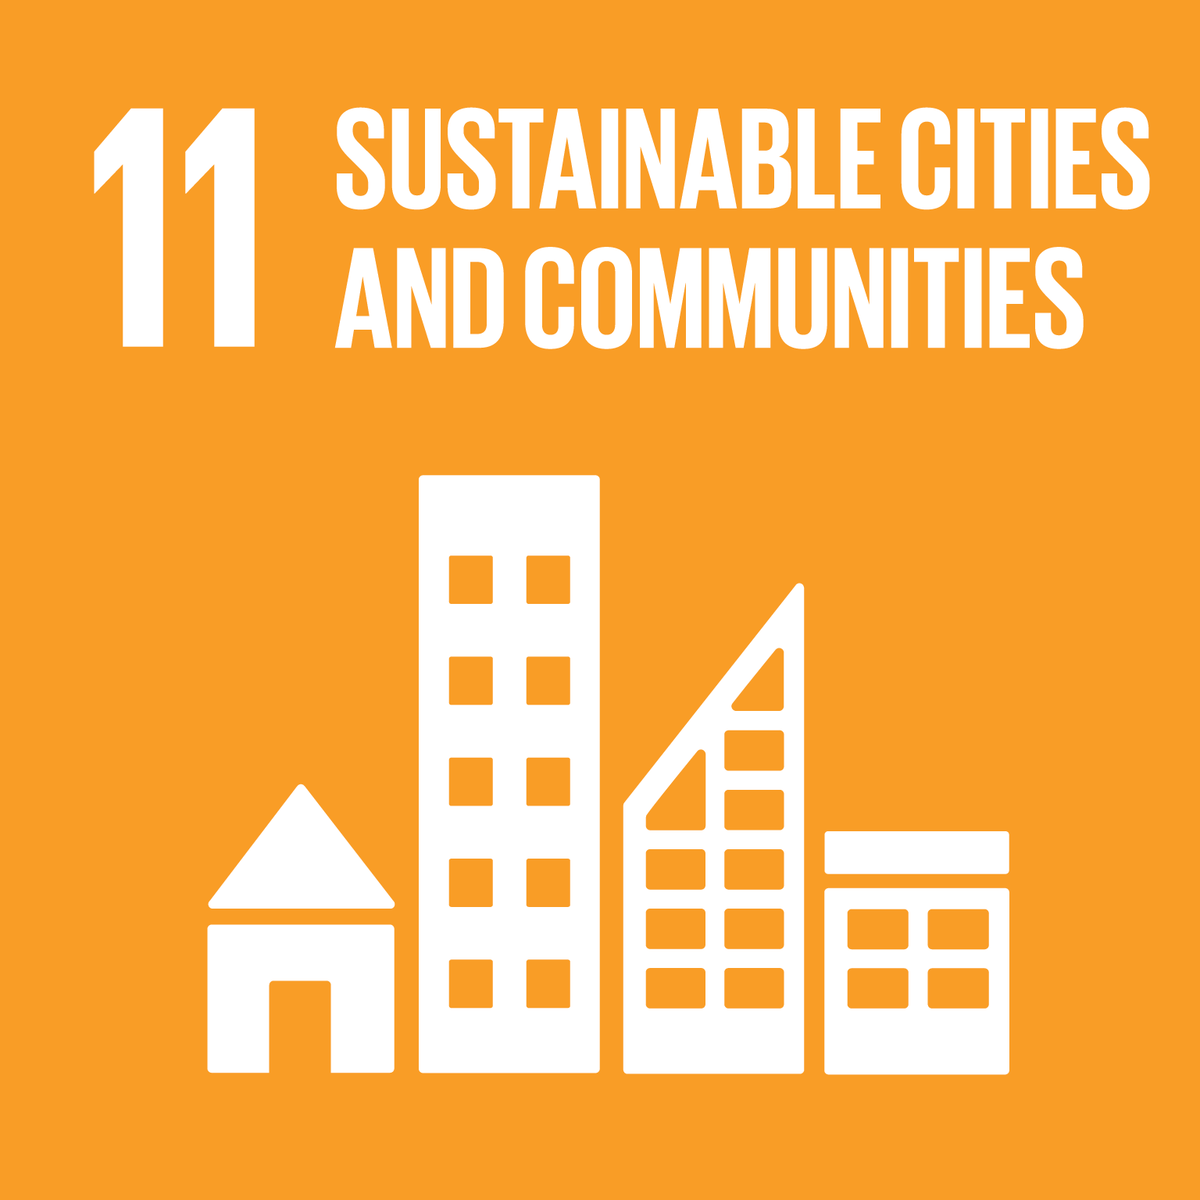
\includegraphics[width=0.3\textwidth]{Figures/sdg11.png}
    \caption{Sustainable Cities and Communities}
    \label{fig:2}
\end{figure}

\section{Constraints}
Although Sighteo is a promising project, some of its limitations are listed below:

\begin{itemize}
    \item \textbf{Environmental Factors}: Lowly lit / crowded environments, and presence of fast moving obstacles may cause inconsistencies in detections.
    \item \textbf{Dataset Limitations}: Specialized datasets for visually impaired navigation are highly limited. This may require us to adapt or create a custom dataset.
    \item \textbf{Testing Environment}: Initial deployment will focus on controlled or semi-controlled indoor spaces. This may be expanded to testing in complex outdoor environments in future.
    \item \textbf{User-Centered Design Issues:}: Designing for people with visual impairments fundamentally relies on iterative feedback and usability testing with real users. That may not be easily possible.


\end{itemize}

\section{Business Opportunity}
The global assistive technology market is expanding rapidly. This is due to rising awareness of inclusivity. Current solutions rely on costly hardware (e.g., LiDAR sensors) or require constant human intervention, which limits their accessibility and scalability.

Sighteo can be a game-changer by providing a low-cost AI-based navigation system which can be easily availed through the usage of a smartphone. The technology can be integrated in NGOs, hospitals, and smart city initiatives. The increased demand in low-cost and mass-scale assistive technology can transform the project into a business opportunity.

\section{Stakeholders Description / User Characteristics}
The following section identifies key stakeholders in Sighteo and outlines specific roles for each group in the development and impact of the project. We also highlight some goals and expectations of these stakeholders and show how their needs shape the direction of the system. We then give a summary of main problems to be addressed for each group by Sighteo.
\subsection{Stakeholders Summary}
\begin{itemize}
    \item \textbf{Primary Users}: Visually impaired individuals trying to seek safe and independent navigation.
    \item \textbf{Secondary Users}: Caretakers and families with visually impaired individuals.
    \item \textbf{Project Team}: Developers / AI Engineers responsible for tasks like model training, deployment, and application design. Testers for validating the use of our application.
\end{itemize}

\subsection{Key High-Level Goals and Problems of Stakeholders}
\begin{itemize}
    \item \textbf{Visually Impaired Users}: Need a reliable real-time navigation support for reducing dependency on others. Their main requirement is safety. They will expect precision from the system to trust it.
    \item \textbf{Caregivers and Families}: Want tools that provide assisstance reducing their own involvement. Their concern may be affordability and ease of use.
    \item \textbf{Developers / Researchers}: Aim to deliver robust on-device system. The system must be capable of handling real-time object detection. Their challenge is balancing accuracy, latency, and connectivity requirements.
\end{itemize}

\section{Conclusion}
In this chapter, the motivation behind our Sighteo, the scope of work, and the direction taken have been elaborated. The challenge faced by visually impaired individuals was identified, and an approach toward solving this problem was formulated within the context of being affordable, accessible, and offering real-time indoor navigation. The problem domain was outlined, the goals of the system were outlined, and its socio-economic significance was highlighted against the backdrop of global development goals too in the text.

\chapter{Literature Review / Related Work}
This chapter documents past literary works and existing technologies in the domain of assistive navigation technology for visually impaired individuals. Through this literature review, we aim to identify trends, strengths, and limitations of existing methods and systems. Academic researches were analyzed alongside existing commercial applications to provide a view of the landscape of this project. For each literary work or application, there is a summary, critically analysis comparison with Sighteo. The chapter concludes with summary tables that precisely mentions the findings from each work discussed.


\section{Definitions, Acronyms and Abbreviations}

Some of the important definitions, acronyms, and abbreviations are given below:


    \textbf{CNN:} CNN stands for Convolutional Neural Network. It is a class of deep neural networks widely used for image recognition and classification.\\
    \textbf{VLM:} VLM stands for Vision Language Model. It is an AI model that combines visual and textual data for understanding of context.\\
    \textbf{MR:} MR stands for Mixed Reality. It is a technology that blends real and virtual environments. It is often used in advanced assistive navigation systems.\\
    \textbf{TTS:} TTS stands for "Text to Speech". It is a library that converts text into audio output.\\
    \textbf{ETA:} ETA stands for Electronic Travel Aid. It can be any device that provides information to assist visually impaired users in mobility.\\
    \textbf{EOA:} EOA stands for Electronic Orientation Aid. These are systems that support orientation by providing information about the environment.\\
    \textbf{PLD:} PLD stands for Position Locator Device. It is a device used to track the position of the user during navigation.\\
    \textbf{LiDAR:} LiDAR stands for Light Detection and Ranging. It is a sensor that measures distances using laser by creating three dimensional maps.\\
    \textbf{COCO:} COCO stands for Common Objects in Context. It is a large scale dataset used for object detection tasks.\\
    \textbf{ABF:} ABF stands for Adaptive Bilateral Filtering. It is a technique used to preserve image edges used in pre-processing for Deep Learning Models.\\
    \textbf{BiLSTM:}  BiLSTM stands for Bidirectional Long Short-Term Memory. BiLSTM is a structure which feeds the sequence of the available data in forward and backward passes. It perceives the contextual dependencies.\\
    \textbf{SSAE:} SSAE refers to the Sparse Stacked Autoencoder. It is the deep structure in the neural networks utilized for unsupervised feature learning. It also allows dimension reduction.\\
    \textbf{DNN:} DNN stands for the phrase Deep Neural Network. It's a multi-hidden layer network. It's extensively utilized while working with complex relations and data patterns.\\
    \textbf{IoT:} IoT represents the Internet of Things. It refers to the collection of interconnected devices and sensors that communicate and exchange information in order to benefit from increased system intelligence.\\
    \textbf{UR Fall Detection Model:} UR Fall Detection Model means University of Rzeszów w Fall Detection Model. It can be used for the evaluation of human activity recognition systems.\\
    \textbf{PRISMA:} PRISMA refers to the Preferred Reporting Items for Systematic Reviews and Meta-Analyses. It includes the guidelines for conducting systematic reviews. It also allows for the transparent reporting of the studies.\\
    \textbf{GhostNet:} The GhostNet stands for Ghost Convolutional Neural Network. It's a light-weighted CNN and produces feature maps. The maps assist in minimizing computations.\\
    \textbf{BiFPN:} BiFPN stands for Bidirectional Feature Pyramid Network. It is a feature aggregation module. It is used in object detection.\\
    \textbf{VEO:} VEO stands for Visual Environment Optimization. It is a framework that enhances node selection and path optimization in AI based navigation systems.\\
    \textbf{OCR:} OCR stands for Optical Character Recognition. This computer vision technique extracts text from images and videos.\\
    \textbf{MR.NAVI:} MR.NAVI stands for Mixed Reality Navigation System. It is a platform that integrates MR technology with spatial audio and visual cues.\\
    \textbf{HAR:} HAR stands for Human Activity Recognition. It is the automated classification of human actions like walking or falling from sensor or vision data.\\
    \textbf{Open Images:} Open Images is a dataset of annotated images used for object detection and classification.


\section{Detailed Literature Review} 
This section of the report documents the review of literature consisting of past researches, studies, and existing competing solutions related to assistive navigation for visually impaired individuals. It discusses studies that introduce smartphone-based systems, object recognition applications, and real-time pathfinding algorithms, analyzing their strengths and limitations. Based on a review of previous studies and available market solutions, the framework of our proposed system is established, key gaps are identified, and our study is contextualized as an advancement in AI navigation aids.
\subsection{A Smartphone-Based Mobility Assistant Using Depth Imaging for Visually Impaired and Blind}
It is among the pioneering attempts to explore how a smartphone’s depth sensor can be used to facilitate the movement of visually impaired or blind people. The current research is based on the idea of proving that the use of a phone will enable detection of nearby obstacles through the usage of no additional devices. Due to this integration of sensing technologies into the smartphone, the application under consideration can provide some spatial awareness to its user along with timely warning of possible obstacles.
\subsubsection{Summary of the Article}  
See, Sasing, and Advincula \cite{ref:see2022smartphone} introduced a smartphone-based assistant for visually impaired and blind individuals that utilizes depth imaging technology. The core of their system lies in leveraging the built-in depth cameras of modern smartphones to provide users with spatial awareness and obstacle detection without the need for additional hardware. The technology extracts depth data from 23 coordinate points that are located within the scene that is being captured and then it divides the obstacles into the prescribed zones: head zone, torso zone, ground zone, or full body obstacles. The maximum range for obstacle detection mentioned was 1.6 meters which is the range suitable for being aware of the objects around.

Furthermore, the study not only indicated the possibility of having obstacle-detecting technology for blind people but also unveiled a new feature that helps directing visually impaired people to the areas where they want to look for things. The system applies various kinds of feedback very skillfully by offering the users both sounds and vibrations thus making it appropriate for a wide range of users' preferences. The process design has integrated voice and gesture controls, thus making the interface more versatile and user-friendly with more than 80\% success rate confirming the effectiveness of the proposed method.

\subsubsection{Critical Analysis of the Research Item}  
The study makes significant contributions to the field by examining depth imaging as a means to improve assistive navigation systems. To begin with, the most significant disadvantage of the study is the limited detection range of 1.6 meters, which might be insufficient. Additionally, the system used only 23 fixed coordinate points for collecting depth data, which was a problem from the perspective of reliability. Even though less computationally intensive, this approach might miss small or strangely shaped obstacles. Moreover, while the system alerts the users to the presence of the obstacles, it does not provide them with the means of direction or map planning. The users will have to take navigation decisions themselves, which could still be very difficult in case they are not familiar with the area. Moreover, the visually impaired find the use of voice and gesture inputs as an extra cognitive load. A person with impaired vision may find it hard to give a voice command or perform a gesture to change the system settings. Static object detection and obstacle alerts rather than continuous navigation in dynamic environments, is the main focus of the research. Changes in lighting, reflective surfaces, or multiple moving obstacles are issues which were not deeply analyzed, leaving the robustness of the solution area of concern under real-world conditions.

\subsubsection{Relationship to the Proposed Research Work}  
The most intuitive way of providing feedback is revealed by the new methodology of categorizing hindrances as particular body zones. However, several shortcomings can be found in See et al.'s \cite{ref:see2022smartphone} study that serve to guide our future project towards specific areas of interest. Namely, despite covering indoor and outdoor settings, the system does not offer the necessary assistance especially in the case of indoor environment because of narrow corridors, odd arrangements of furniture, and cluttered obstacle. In our project, we will concentrate solely on indoor conditions. Also, contrary to See et al., whose main objective is to alert users of obstacles, our future application will strive to actively help its user navigate through indoor space by suggesting the safest possible path and navigating directions. Finally, while the authors utilize a predetermined coordinate system of points in detecting obstacles, we will apply a more sophisticated system using the methods of object detection in order to achieve greater precision in recognizing obstacles. Nevertheless, See et al.'s \cite{ref:see2022smartphone} study laid a strong foundation by establishing the usefulness of depth imaging technology on smartphone for aiding visually impaired people. However, the limited detection distance, lack of directional cues, dependence on fixed points and emphasis on multimodal control leave much room for improvement.
\subsection{Android-Based Object Recognition Application for Visually Impaired Users}
This paper introduces a modest attempt to create an Android app based on object recognition technology that can cater to the requirements of people with visual impairments. It attempts to emphasize the deployment of light-weight models to the local device without using any cloud computing services so that assistive applications can become cost-effective and accessible to a wider range of people. Using the approach of providing object detection through audio, this research highlights a possible solution for assisting visually impaired people to understand their surroundings better.

\subsubsection{Summary of the Article}
Bhagwat et al. \cite{ref:salunkhe2021android} introduce an Android app in this research that is intended to assist visually challenged users in comprehending their environment. The app detects objects in real time. It grabs the live video frames from the camera of the smartphone. Utilizing TensorFlow's Object Detection API, it identifies objects on the scene. The model is transformed into TensorFlow Lite. This enables offline, device-local processing, eliminating reliance on cloud or network availability. Once an object is recognized, it is converted into an audio cue using the device's Text to Speech (TTS) engine. The authors claimed that about 90 percent accuracy was achieved by the system in object detection in their test cases. The paper also describes a component for real-time text reading (recognizing printed text in the live scene) alongside object recognition, although the primary focus is object detection and voice feedback.

\subsubsection{Critical Analysis of the Research Items}  
In this paper, the authors show a practical method for implementing object detection in a mobile app that has offline functionalities. Using the SSD architecture is a great decision for resource-limited environments. The choice of Tensorflow Lite is an indicator that the developers are aware of the issues related to the practical deployment of mobile applications. However, the limitations of the system in terms of design, evaluation, and claims become clear on careful examination. Firstly, the 90\% accuracy they claim is not only about false positives, latency, or performance in difficult indoor conditions like low light, occlusion, or clutter. It mainly concerns either static scenes. Secondly, the system only informs the user about the names of the objects only. No help in navigation is provided. Thirdly, the device does not account for moving obstacles. Fourthly, there is no discussion about performance measures, including frame rate and energy consumption, that are necessary for any assistive devices. Moreover, although reading the text is also an excellent addition, the authors do not discuss how accurate the text recognition will be in case of varying light intensity, tilting of the surface, or curved surface. Furthermore, the transition from object detection to text reading can significantly impact the user experience. The usability of the device under real-world conditions, especially when walking through a room containing multiple objects and surfaces, is not fully examined in the article.
\subsubsection{Relationship to the Proposed Research Work}  
Bhagwat et al.’s \cite{ref:salunkhe2021android} work provides a great reference point and a technolical baseline. It demonstrates the feasibility of running object detection and voice feedback in real time on a mobile device. It establishes the fact that mobile phones can handle object recognition without relying on server infrastructure. However, the gaps in their work align closely with the problems Sighteo aims to solve. Their system stops at object identification and vocal naming. It does not go further into active navigation guidance. And, that is central to our goal. Because Bhagway et al. do not consider indoor specific constraints such as tight hallways, clutter, floor level hazards, or moving obstacles, their design is generic. Sighteo will build on this foundation. Through Sighteo, we aim to enhance performance providing continuous directional guidance. We will also focus on minimising latency, which was not the focus in this paper. After establishing that object recognition on a phone for the visually impaired is indeed possible, the paper leaves an open challenge of converting that recognition into safe real time navigation.

\subsection{Efficient Real-Time Pathfinding for Visually Impaired Individuals}
This work redirects focus from mere obstacle detection to the computation of safe real-time paths for visually impaired users. This research is not only interested in creating awareness but also focuses on the use of algorithms for navigating dynamic environments using collision-free paths. The approach highlights the importance of low latencies, adaptability, and efficient computations. Effective pathfinding proves essential for constructing a framework for enabling live navigation services. In general, the approach illustrates that computing real-time routes helps improve movement over and above object detection.
\subsubsection{Summary of Research Item}  
In this paper, Ghahremanians and Mohammadi \cite{ref:ghahremanians2025efficient} introduce a method for effective real-time path planning specifically for visually impaired persons. The main concern of their research is the calculation of safe routes for users without any collision throughout their journey amid obstacles or even dynamic objects. This method tries to combine various issues such as low delay time, efficiency in computations, and flexibility with environmental changes. The introduced algorithm is intended to be executed in real time, which makes it more suitable for real-time guidance rather than route planning.

\subsubsection{Critical Analysis of the Research Item}  
This study is important because it solves the critical problem of turning obstacle data into feasible paths rather than object recognition alone. Most earlier studies would stop at notifying the user about an object, but in this case, the challenge is to figure out how the person can walk safely by avoiding collision. The emphasis on real-time operation indicates that the researchers recognize the need for quick responses, which can be crucial in navigation assistance. Negative aspects are that the publicly available summaries are uninformative about precise evaluation outcomes, particularly under indoor, cluttered, or dynamic conditions. It's also indeterminate how uncertain or noise-laden input (e.g. from a moving-camera phone's camera) is handled. Another drawback is whether the technique presumes a mapped environment (or pre-known layout), versus operating in arbitrary, unseen spaces. Furthermore, the paper apparently targets quite widely (for general visually impaired navigation); we are not clear that it's particularly optimized for indoor limitations such as narrow hallways, objects at the person's level, or overlap furniture. The computational efficiency claims are promising, but we are uninformed about memory usage, energy usage, or how well it tolerates latency in low-spec devices (e.g. phones). Lastly, dealing with dynamic objects (moving people or moving objects) represents a serious practical problem, and it's indeterminate from the summary how stable their method is in this respect.

\subsubsection{Relationship to the Proposed Research Work}  
This research in specific is up-to-date since it fills the gap in the literature from obstacle detection up to path planning. In regards to our proposed application, their study provides us with a way on how to calculate in real time the safest possible route based on the information coming from sensors. The study reveals that path finding may actually be one of the most significant components of the system and not just a concept that is made up for the purpose of academic research. On the other hand, our application has a large number of unique features which apply exclusively to our application alone. Our application focuses on indoor navigation. The approach described by Ghahremanians and Mohammadi \cite{ref:ghahremanians2025efficient} does not limit its applicability for indoor-only use and thus potentially overlooks some indoor-specific issues. Additionally, our application is intended to provide unobstructed guidance (directions, avoidance maneuvers) during user movement, perfectly synchronizing with user detection rather than relying on prior mapping or grand outdoor-style planning. Their approach is based on efficiency; thus, we are able to employ their strategies for latency reduction or simplified path planning but we need to make sure that they are adapted to effectively work in the challenging situations created by noisy, occluded, and rapidly changing indoor mobile camera input. To put it briefly, the research by the authors is useful for our path planning part of the algorithm, yet we have to improve it in terms of indoor navigation, tight connection with object recognition, as well as user-friendly feedback via sounds and vibrations.


\subsection{Improved YOLOv5 Algorithm Combined with Depth Camera and Embedded System for Blind Indoor Visual Assistance}
This study focuses on enhancing the capabilities of YOLOv5 through the fusion of depth sensing data, optimization of embedded hardware, and architecture modifications in order to develop indoor assistance applications. The researchers explore the way depth sensors may improve object detection accuracy in case the environment is cluttered or the distance between objects and the camera is minimal. Furthermore, the role of architecture modifications in reducing computations without loss of accuracy and making the system suitable for indoor application on embedded devices is emphasized.

\subsubsection{Summary of the Research Item}  
Zhang et al. \cite{ref:zhang2024improved} propose an enhanced YOLOv5 algorithm integrated with a RealSense D435i depth camera and a Raspberry Pi 4B to create an indoor assistive system for visually impaired individuals. Their approach replaces the YOLOv5 backbone with GhostNet to reduce parameters, incorporates a coordinate attention mechanism for better feature representation, and uses a bidirectional feature pyramid network (BiFPN) for improved feature fusion. In comparison with the baseline YOLOv5s models, the upgraded version reduces the size by 42.4\% and the number of parameters by 47.9\% while improving the recall by 1.2\% and keeping the precision stable. The system also accommodates voice input and yields audio feedback with object detection and ranging, making the system more suitable for use in everyday indoor applications among the visually-impaired.

\subsubsection{Critical Analysis of the Research Item}  
One of the key advantages of the work is the good tradeoff between detection accuracy and computational efficiency such that the system can be run on handheld devices such as Raspberry Pi. The combination of the GhostNet and the BiFPN shows good architectural innovation in attaining light-weight design and stable performance. The incorporation of a depth camera also corrects one key weakness in the literature on 2D vision systems, which is the inability in the state-of-the-art literature to estimate distances accurately. Despite the foregoing advantages, the system does have some key weaknesses. Its training dataset is quite small and comprised only of some indoor objects (e.g., bottle, cup, key), so generalization is limited. In addition, low-light and speech accent variations cause concerns in the usability in the real world. Even though the work was conducted in highly restricted indoor conditions, questions remain about its scalability and robustness in more varied and more complicated conditions.

\subsubsection{Relationship to the Proposed Research Work}  
This work immediately relates with our project concept as it validates the possibility of combining embedded devices and computer vision in the assistive navigation task. Even though our system utilizes the smartphone camera, and not a depth camera, the architectural optimizations proposed in Zhang et al. \cite{ref:zhang2024improved}  provide potential directions in the tradeoff between computational load and precision. In its concern with fusion of auditory feedback and real-time object detection, its orientation also strongly corresponds with our aim in the provision of intuitive direction-finding assistance to the visually impaired.

\subsection{Assistive Navigation Technologies: A Comprehensive Overview}
The present paper gives a brief description of the assistive navigation technologies designed for the visually impaired. The present paper describes a great number of solutions that have been already developed; also, there is a classification based on the types of sensing, architecture of systems, and ways of interaction with the users. Thus, an insight is provided into how the sensors and feedback mechanisms can be applied within the existing solutions. The broad overview helps highlight the benefits of the currently available technologies and areas that require further research.

\subsubsection{Summary of the Research Item}  
The authors Abidi et al. \cite{ref:abidi2024comprehensive} in this research paper have cited the works of researchers that have explored various types of devices which help the visually impaired people. Such devices can be either wearable like haptic vests and smart glasses or non-wearable like navigation sticks and sensor system. While both RGB-D cameras and tactile sensors can be used to help the visually impaired understand their environment better, Internet of Things and satellite-based guidance allows multiple users at a time to use the system \cite{ref:abidi2024comprehensive}. Moreover, from the results of the study, it is evident that human-centered design is an essential element that leads to a better quality of life of blind people \cite{ref:abidi2024comprehensive}.

\subsubsection{Critical Analysis of the Research Item}  
One of the most important advantages of this paper is the comprehensive classification of contemporary solutions and discussion of the technical basis of such solutions, which creates a firm base for future studies. Nevertheless, while this paper extensively reviews contemporary technologies, it does not critically address the weaknesses inherent in deploying them in the real world, such as Internet connectivity and cost, among others.

\subsubsection{Relationship to the Proposed Research Work}  
From our standpoint, this review serves as an excellent benchmark, since it emphasizes the significance of incorporating technologies that use artificial intelligence and mobile solutions for blind navigation. The fact that we are developing a solution that would leverage a phone camera to give navigation instructions makes the results highly relevant for us, especially in terms of practical problems such as connectivity issues, which were completely ignored by the authors \cite{ref:abidi2024comprehensive}.

\subsection{Assistive Systems for Visually Impaired Persons: Challenges and Opportunities}
The purpose of this review is to describe some of the major problems inherent in designing good assistive technology and how modern sensor technology and AI can provide opportunities to overcome them. Some of these include accuracy and reliability concerns as well as user comfort and functionality problems. There are also opportunities presented through new hardware capabilities in mobile devices and new light-weight machine learning approaches. Overall, this review highlights several key factors which will ultimately determine usability and adoption of these systems.

\subsubsection{Summary of the Research Item}  
The study by Okolo et al. \cite{ref:okolo2024assistive} provides a literature review focusing on the problems and potentials associated with designing assistive systems for blind people, specifically navigation tools. According to the paper, assistive technology can be divided into three categories – sensing input devices (such as smartphone, radio frequency identification (RFID), depth camera, infrared sensor, ultrasonic sensor, and RGB-D sensors), feedback interfaces (auditory, tactile, vibro-tactile, haptic interface), and IoT-based assistive technology. In addition, the authors suggest the necessity of the integration of artificial intelligence, computer vision, and mobile technologies in order to advance the development of assistive tools for navigating obstacles and gaining an understanding of the environment.

\subsubsection{Critical Analysis of the Research Item}  
This research is unique due to the fact that it makes detailed classification of various technologies and makes comparison between the AI-powered and IoT devices. In addition to just listing the technology types used, the study points to their drawbacks in terms of bulky nature, high cost, poor efficiency under bright light, and difficult user acceptance. However, while the study contains mostly theoretical knowledge, there are no practical insights about the usability of the systems. Also, although it makes future predictions regarding multi-modal feedback and mobility, the research fails to provide clear guidance on designing systems.

\subsubsection{Relationship to the Proposed Research Work}  
The paper is also very relevant to our concept since it identifies the need for mobile and AI-enabled navigation technology. Our system makes use of a phone camera for detecting obstacles and directions, and therefore the outcome, regarding the drawbacks of vision-based systems (such as the inability to estimate depth with normal cameras), perfectly fits our expectations regarding the technological limitations we should overcome. Furthermore, the recommendation for light, userfriendly, and portable systems corresponds well with our goal of developing a feasible, smartphone-based navigation system specifically with the visually impaired in view \cite{ref:okolo2024assistive}.

\subsection{Technological Advancements in Human Navigation for the Visually Impaired: A Systematic Review}
In this systematic review, the latest progress made in navigation technologies targeted at the visually impaired is described to provide a broader technological background and perspective on contemporary developments in this field. Specifically, the latest trends in sensory capabilities, positioning, and feedback approaches are illustrated, as well as the patterns that can be found across a wide variety of navigation devices are shown. At the same time, this review indicates important limitations that continue to prevent the implementation of these devices widely owing to problems with usability, cost, or performance.

 \subsubsection{Summary of the Research Item}
Casanova, Guffanti and Hidalgo \cite{ref:casanova2025technological} provide a systematic review of 58 recent works from 2019 to 2024 on assistive navigation technologies for the blind and visually impaired. The authors emphasize that while advanced sensors and artificial intelligence driven systems are growing in importance, the current state remains such that people with blindness and visual impairments are far from fully benefited in terms of access and inclusivity. The review synthesizes the major innovations such as the integration of high-precision GPS with ultrasonic sensors, Bluetooth and haptic feedback systems, and deep learning-based algorithms for obstacle avoidance and route planning. The review lists the range from the simplest screen reading and navigation app assistance to the latest smart cane, smart shoe, smart belt and LiDAR-based technologies. Some examples are BlindRouteVision, which integrates Android apps with GPS and ultrasonic sensors, and wearable systems based on Raspberry Pi technologies that implement fuzzy logic and vibrotactile feedback for real-time safe navigation.

\subsubsection{Critical Analysis of the Research Item} 
Some of the important strengths that characterize this review include the systematic and comprehensive nature of the discussion where the PR the Accept Dismiss ISMA protocol (used for improving the clarity of systematic reviews and meta-analyses reports) was utilized to ensure rigor in the process. The review categorizes solutions as smartphone-based technology, haptic interfaces, and artificial intelligence-based navigation aids. In addition, it indicates that the majority of the surveys included in this review had experiments to support their conclusions, with 79 percent of all the surveys included using experimental validation, where the most common type was haptic feedback. Finally, the weaknesses in current technologies discussed indicate future directions for development.

\subsubsection{Relationship to the Proposed Research Work}  
This project directly ignites our project Sighteo's mission. It validates our decision to combine AI-powered object detection with audio and haptic feedback and sheds light on the gaps we aim to close, notably improving indoor navigation and designing with affordability and access in mind. We are building on the literature's strengths and aiming to avoid the weaknesses in order to create a useful solution.

\subsection{Assistive Systems for Visually Impaired Persons: Challenges and Opportunities}
This section looks into the various machine learning systems developed for visually and hearing-impaired people. It underlines how new models contribute to recognition and perception and, in general, to accessibility. Much importance is given to the way these technologies interpret an environment surrounding real life, classify sounds, and assist in daily navigation, with an increased role being given to deep learning for accuracy and responsiveness.

\subsubsection{Summary of the Research Item}  
Patel et al. \cite{ref:patel2025enhancing} give an overview of machine learning methodologies used to aid visually and hearing-impaired people, including classic ML and deep learning. For audio, they discuss how models such as SVM, Random Forests, and MLPs can be applied for speech and sound classifications. In terms of visual analysis, they provide a breakdown of models that perform real-time object detection, such as YOLO, SSD, and RetinaNet, for the purpose of scene understanding and navigation support on wearables and mobile phones. The paper further highlights examples of Generative AI usage and notes that, in order for these models to be effective, fine-tuning and customization are essential. Overall, the authors' work reflects a pattern starting with devices, datasets, and algorithms before moving on to applications.

\subsubsection{Critical Analysis of the Research Item}  
The strengths of the paper include its consideration of both sensory modalities and methodical separation of approach by task and modeling paradigm, making this a good paper to consult in choosing models. The paper is also interested in the problem of real-time requirements and the need for model-specific tuning, bringing one very close to realistic applications. However, being a general review article, it does not present direct performance comparisons based on common testing methodology, so performance can only be estimated from a set of other works. Constraints on processing due to battery life and overheating and discussions of user study are limited, and the problems of long-term adoption and costs are still not resolved.

\subsubsection{Relationship to the Proposed Research Work}  
Given that the focus of Sighteo involves indoor navigation, this paper reiterates that we should be using state-of-the-art object detection models such as YOLO, SSD, RetinaNet, while also determining which data set can work best to achieve balance between accuracy and efficiency. The other piece of advice offered is that we need to consider early on how personalization can help us in our application, as most assistive devices make use of thresholds that can be adjusted by users.

\subsection{Ensemble of Deep Learning and IoT Technologies for Improved Safety in Smart Indoor Activity Monitoring for Visually Impaired Individuals}
The proposed combination of deep learning and IoT-based activity monitoring for indoor use is presented here in the literature. Even though it does not have anything to do with navigation, it helps us understand more about using a combination of models, namely sensor fusion, to provide greater safety and situational awareness for the user who has a visual impairment.

\subsubsection{Summary of the Research Item}
The author Al Duhayyim \cite{ref:al2025ensemble} presented a novel IoT and deep learning based ensemble model called EDLES-SIAM (Ensemble of Deep Learning for Enhanced Safety in Smart Indoor Activity Monitoring). This system uses an ensemble combination of deep learning models such as Deep Neural Network (DNN), BiLSTM, and SSAE to recognize human activities (HA) accurately. In this model, the process of feature extraction begins with the application of Adaptive Bilateral Filtering (ABF) to remove noise from sensor data and images. Feature extraction is carried out with ResNet50, which extracts features from images. Finally, the result of the ensemble is obtained by adding the output sequentially to detect HA, as well as abnormal HA, such as falling and unsafe movement. The model was tested using the UR Fall Detection dataset, yielding classification accuracy of 99.25\%. Compared to single deep learning algorithms, such as VGG16, VGG19, and some ResNets, the proposed algorithm showed higher accuracy. The study reveals how individual IoT and deep learning-based systems make significant contributions to monitoring visually impaired individuals.

\subsubsection{Critical Analysis of the Research Item}

The strength of this study is that it uses both recurrent network and autoencoder for its strength in temporal processing as well as CNN network in terms of features extraction, which allows the application of this model in real time. The application of the adaptive bilateral filtering (ABF) technique also increases image quality, which means increased accuracy. However, one major drawback of this model is its high cost, making it unsuitable for smartphones. Relying on a single dataset (UR Fall Detection) in an effort to reduce generalization to more varied environments is another restriction. In addition, the lack of user trials involving visually impaired users ensures that real-world usability, latency, and energy efficiency of the system are not realized. Although the findings are encouraging for smart indoor safety, accessibility and scalability continue to be key challenges. 

\subsubsection{Relationship to the Proposed Research Work}

Al Duhayyim's \cite{ref:al2025ensemble} work is of direct applicability to the suggested smartphone-based navigation system, as it illustrates how ensemble deep learning may enhance the perception model's robustness used for assistive safety. The idea of combining deep learning with IoT-based sensing supports the significance of multi-modal data in improving situational awareness. Yet, in contrast to EDLES-SIAM based on high-performance IoT configurations and ensemble computation, the suggested project seeks to provide real-time perception based on only a martphone camera and a light AI model compiled for mobile. It ensures affordability, mobility, and freedom from external sensors or high-end edge hardware. Observations from this work affirm the worth of preprocessing, feature integration, and ensemble learning concepts but call attention to the need to streamline these processes for low-power, real-time application applicable to daily use by the blind. 

\subsection{VocalEyes: Enhancing Environmental Perception for the Visually Impaired through Vision-Language Models and Distance-Aware Object Detection}
This work introduces an assistive system that incorporates vision-language models into a distance-aware detection pipeline. It demonstrates how spatial information significantly enhances contextual understanding and increases the environmental awareness of the user. By offering more descriptive and meaningful feedback, this departs from the simple detection of objects and provides a richer interpretation of the surroundings, one that's particularly valuable for assistive navigation.

\subsubsection{Summary of Research Item}  
Chavan et al. \cite{ref:chavan2024vocaleyes} propose VocalEyes, a real-time assistive system designed to improve situational awareness for visually impaired individuals. The system uses a quantized and fine-tuned Florence-2 large vision-language model, optimized for 4-bit accuracy, to process the live video input and make the deployment on low-power devices like the NVIDIA Jetson Orin Nano. With a latency of 5 frames, the system is capable of giving contextual descriptions of objects, pedestrians, and obstacles, distance estimation included. For feedback purposes, it has incorporated Parler TTS Mini, a compact text-to-speech engine that supports 34 different speaker types and offers customizable voice styles, thus giving audio guidance that is user preference-based. The research considers the system's accuracy, efficiency, and usability and gives an impression of it being a real-time, low-cost navigation support solution.

\subsubsection{Critical Analysis of the Research Item}  
The ability of this project to modify a massive model (Florence-2) to run at the edge is among the main advantages that stand out. The system performs fine-tuning and quantization for efficient and contextually accurate operations. Besides pointable object identification, value-added functionality in this case is given through the distance-sensitive detection and personalized TTS with a customizable voice option. However, certain limitations can be found. For example, the necessity for an NVIDIA Jetson system is somewhat limiting as far as mobile phone implementation is concerned. Also, the 5 frame latency is fairly low, but still might cause responsiveness issues in dynamic environments. Finally, while much attention is paid to accuracy and efficiency performance, little discussion is dedicated to more advanced studies in real-life situations.

\subsubsection{Relationship to the Proposed Research Work}  
VocalEyes \cite{ref:chavan2024vocaleyes} is a major reference for our project. It illustrates the great potential of tuning large AI models to be used in real-time assistive applications. The system works on top of edge hardware but we are striving to provide similar features, namely contextual object detection and real-time feedback, with the help of a smartphone camera only, to make the system available at a larger scale. The use of distance measurement and adaptive voice feedback in VocalEyes is very much in line with the intent of offering easy and lovable navigation support to the user. On the other hand, the problems of hardware dependence and latency raised in the research pointed out that developing lightweight, mobile-optimized solutions that are independent of external processing devices becomes even more important, and this is exactly where our focus of research is.

\subsection{MR.NAVI: Mixed-Reality Navigation Assistant for the Visually Impaired}
This paper discusses using mixed-reality headsets for navigation. It combines spatial audio, object detection, and real-time guidance in a single wearable device and lets the user receive constant and intuitive support while he or she moves around complex environments. Blending virtual cues with real-world perception, it underlines how mixed reality has the potential to give visually impaired individuals a more confident and informed way to navigate.

\subsubsection{Summary of Research Item}  
MR.NAVI from Pfitzer et al. \cite{ref:pfitzer2025mr} is described as a mixed reality-based navigation system intended to improve spatial awareness and navigational abilities for people who are visually impaired. This tool can be characterized as a complete navigation assistance system combining features of computer vision, natural language processing, and spatial audio output. As a software product, MR.NAVI is built upon the Microsoft HoloLens2 hardware, using features such as object detection, depth estimation, obstacle avoidance, and even public transport route planning under a unified architecture. Thus, MR.NAVI works both as an Electronic Orientation Aid (EOA), Electronic Travel Aid (ETA), and Position Locator Device (PLD) at once, covering the gap which currently exists since many systems only offer either EOA or ETA functions, and none PLD functionality. In addition, MR.NAVI outputs information regarding scene descriptions, navigation, and collision avoidance in both visual and auditory forms, with voice commands used as a primary means of communication between the system and its users.

\subsubsection{Critical Analysis of the Research Item}  
One of the strengths of MR.NAVI is that it incorporates all the features of EOA, ETA, and PLD into one system and many others do not have the same level of integration as this. The application of multimodal feedback with the use of spatial audio, visual indication, and natural language responses made it possible for the system to be usable for different visual impairments. However, the use of HoloLens2 indicates a pragmatic approach rather than building an overly specialized system. Nonetheless, this reliance on HoloLens2 raises some issues regarding access since the product is quite expensive and not portable as a smartphone alternative. The need for high Wi-Fi connection and use of a server to process the computing-heavy tasks raises doubts concerning the practicality of the application in real-life settings. While the user studies proved helpful, they did not involve users with any form of blindness but blindfolded users only. Besides, the outside use of the system suffered from lighting issues.

\subsubsection{Relationship to the Proposed Research Work}  
The implications of the results generated from MR.NAVI \cite{ref:pfitzer2025mr} have significance towards the design of the targeted smartphone based navigational system named Sighteo. Whereas MR.NAVI highlights the potential that lies in combining the power of multiple assistive technologies under one platform, the dependency of the platform on mixed reality technology hardware is a major downside that may affect the mass application of this model. On the other hand, our research seeks to recreate the capabilities of the platform using the minimum required amount of hardware which includes the use of the smartphone camera alone making it affordable and portable. Another similarity is seen in the choice of natural guidance approaches (i.e., spatial audio and natural language feedback). However, where MR.NAVI focused on simulated environments as well as server side computation for real time processing, Sighteo will incorporate mobile optimization in order to reduce the amount of computation required for real time processing.

\subsection{Visually Impaired Aid using Convolutional Neural Networks, Transfer Learning, and Particle Competition and Cooperation}
This research introduces an innovative technique that utilizes the benefits of convolutional neural networks, transfer learning, and a cooperative particle approach in order to improve object classification capabilities. In the effort to develop a system capable of offering more accurate results, the researchers integrated the above technologies. This article demonstrates how layering technology innovations can result in improved system performance.

\subsubsection{Summary of Research Item}  
Breve and Fischer \cite{ref:breve2020visually} present a system that leverages convolutional neural networks (CNNs), transfer learning, and a novel particle competition and cooperation algorithm to support visually impaired individuals in navigation tasks. For the suggested method, the first step is to apply CNNs for environment object detection and classification, this ultimately leads to the identification of both the barriers and the related contextual cues. The transfer of knowledge from one field to another is also utilized in the form of a pre-trained model in deep learning thereby increasing the precision of the output. Besides this, the particle competition and cooperation strategy is another technique that positively influences the decision-making process regarding the object classification. The combination of the methods enables the system to produce more robust and accurate identification of environmental landmarks than individual CNNs. Their work demonstrates that the integration of multiple AI techniques can make a huge difference in assistive navigation systems.

\subsubsection{Critical Analysis of the Research Item}  
Firstly, the main novelty introduced by this research is that of the hybrid approach where convolutional neural networks along with the concept of transfer learning are combined with particle competition and cooperation to increase the classification performance. This particular choice of methodology is designed to solve common problems such as small sample sizes and low generalizability under real-world conditions. Transfer learning minimizes the need to invest a lot of funds into training the algorithms, thus improving the scalability of the algorithm. However, due to the high computational demands of deep learning in the model, it may be difficult to apply the algorithm in real time, even in devices such as smartphones. Finally, although the paper discusses mostly classification and detection of objects, it does not incorporate any feedback from end-users when using the navigation aid.

\subsubsection{Relationship to the Proposed Research Work}  
In relation to our project, Breve and Fischer's paper \cite{ref:breve2020visually} serves as a helpful reference in how we can utilize transfer learning along with CNNs to enhance the accuracy of our object recognition system in an assistive context. This is because their approach effectively demonstrates the strength of several algorithms improving efficiency. However, their method addresses only the problem of recognition accuracy, while ours is an extension of theirs in which we add navigation support, collision avoidance, and feedback through auditory/haptic senses. Our approach seeks to circumvent the need for significant computing resources in their case by employing a less intensive approach through AI-based object detection.

\subsection{Enhancing Indoor Navigation for Visually Impaired Individuals with an AI Chatbot Utilizing VEO Optimized Nodes and Natural Language Processing}
This paper demonstrates the development of a conversational indoor navigation system that employs an AI-based chatbot. The system operates on natural language processing and a node network customized for the surrounding environment to offer users instructions in the form of voice commands. In this particular case, the system demonstrates how conversational navigation can be made easier for visually impaired people through familiar interaction patterns.

\subsubsection{Summary of the Research Item}

Thandu and Rathinam \cite{ref:thandu2024enhancing} also introduced an AI indoor navigation system that leveraged Natural Language Processing (NLP) and VEO (Virtual Environment Optimization)-optimized nodes in order to guide visually challenged people through an interactive chat-like interface. The system automatically navigates individuals indoors with the help of verbal search commands and navigates in conversation. Interaction of the chatbot occurs with a group of nodes, which have been optimized using VEO and are effectively connected to the environment, thus offering the possibility of generating paths according to the varying scenarios of navigation. With the use of NLP techniques, the chatbot will be capable of identifying user intent and providing feedback accordingly. The entire approach is solely aimed at making indoor navigation more intuitive and interactive by means of dialogue-based support that in turn would lessen the barrier between accessibility and user engagement. The findings from the experimental study showed that this system not only had a very high response accuracy rate but also decreased disorientation of users when compared to the case of static voice guidance techniques.

\subsubsection{Critical Analysis of the Research Item}
The main merit of the work of Thandu and Rathinam is the hybridization of conversational AI with the already present indoor navigation in real-time. The system using NLP provides an apt and more human-like way for the visually impaired people to ask for directions as well as get guidance. The feature of having VEO-optimized nodes incorporated in the system allows the computing of the path to be done faster and the environment to be more adaptable. On the negative, the model only browses through communication and route response whereas it can also serve low-level perception tasks such as obstacle detection and environmental sensing. Due to this fact, the use of the device in such environments where visual feedback or real-time avoidance of hazards is a requirement becomes less suitable. Moreover, the researchers didn't state anything regarding latency, fault tolerance, or noise robustness performance indexes which are all essential for the assistive technologies. Another point indicating reliance on mapping from preset nodes is the low scalability for bigger or unmapped indoor spaces.

\subsubsection{Relationship of the Proposed Research Work}
The contribution by Thandu and Rathinam \cite{ref:thandu2024enhancing} is fundamental to the development of Sighteo in that it expands the scope of assisted navigation to incorporate AI-based communications that are interactive in nature. While the Sighteo system being considered operates on object detection through the use of a smartphone camera with an aim to foster spatial awareness, the possibility of integrating a conversation interface for guidance may arise in the future. From the results of the research conducted, it becomes evident that there is a need for adaptive user-centric feedback systems that will aid in fostering navigational compliance. The Sighteo system embraces this and goes ahead to incorporate visual perception-based navigation instead of using maps.

\subsection{Smart Assistive System for Visually Impaired People: Obstruction Avoidance through Object Detection and Classification}
The article outlines an intelligent assistance system that utilizes both object detection through ultrasound sensors and ensures secure navigation for the blind. Using the information obtained through visual and sound perception, the system provides the user with audio signals about possible obstacles on their way.

\subsubsection{Summary of the Research Item}
Masud et al. \cite{ref:masud2022smart} presented a new technological framework called smart assistive that would facilitate the visually challenged people's way through the environment by detecting and classifying the objects in their way. The amalgamation of computer vision and deep learning algorithms makes it possible to identify the nearby objects and classify them according to the risk level or distance in real-time. An ultrasonic sensor works alongside the stereo vision camera to get spatial information, which is then processed with a convolutional neural network (CNN) for the identification of the object. Upon detection of obstacles, the auditory feedback module notifies the user with spoken alerts about the type and distance of the obstacle. The system was tested in both indoor and outdoor scenarios and reached a high object recognition accuracy and a low latency rate, which resulted in the effectiveness of the system in terms of obstacle detection and collision prevention. The authors pointed out the great potential of using a combination of vision and sensor-based data for creating a robust assistive navigation system.

\subsubsection{Critical Analysis of the Research Item}

One of the main benefits that arose from the research conducted by Masud and his colleagues is the hybrid sensing technique based on vision and ultrasound data that boosts reliability in situations with rapidly changing light conditions or partial visibility. The synchronization of real-time object detection with audio feedback indicates that it is suitable as a working tool for the navigation in daily circumstances. On the other hand, the application of external sensors like ultrasonic modules raises the problem of hardware being more complicated and might also lead to certain questions being raised as to the system's portability and maintenance. The architecture based on CNN, despite being very good in terms of accuracy, still demands a considerable amount of power which makes its usage on low-power mobile devices impossible. The focus of the study is on short-range obstacle detection which is not accompanied by the high-level understanding of pathway estimation or semantic scene interpretation. Moreover, the feedback system is limited to one type of input only, that is audio, which may pose problems in noisy environments or for users with hearing loss.

\subsubsection{Relationship to the Proposed Research Work}

Methodology presented by Masud et al. \cite{ref:masud2022smart} is very in line with the intentions of our project because it deals with the detection of obstacles in real time and gives the user feedback for navigation. Their CNN-based recognition underscores the necessity of computer vision as the main feature of mobility systems. In contrast with Masud's system utilizing several sensors and hardware-specific parts, Sighteo depends solely on the smartphone camera, thus making the solution more affordable, widespread, and simple in deployment. Moreover, the use of haptic feedback in the proposed system also complies with the use of auditory feedback utilized in Masud's work, thus enhancing the usability in varied environments. The current research findings apart from verifying the significance of the fusion among multiple sensors and highly precise object identification also indicate the requirement for light but reliable smartphone-based systems without compromising hardware complexity.


\subsection{Low-Cost Multifunctional Assistive Device for Visually Impaired Individuals}
This work describes the design of a low-cost wearable that can deliver a range of assistive functions integrated on one platform: text reading, obstacle warning, and remote assistance. Thus, it is a multi-functional tool that can serve various daily needs. The authors significantly stress that such systems must be affordable and practical. They emphasize that design decisions are done in support of real-world deployments rather than experimental work alone.

\subsubsection{Summary of the Research Item}
The paper by Kral et al. \cite{ref:kral2025low} describes a pair of smart glasses. This invention combines text recognition, obstacle detection, and remote assistance in one economically-packed system. The device uses a Raspberry Pi Zero 2W as a base and a camera Arducam IMX519 autofocus as well as tactile buttons for user interaction. Immediate audio feedback warns the user about the presence of objects, and text is read aloud to the user to make the user aware of the situation. The invention was needed in a rehabilitation center where its performance in tests had been very accurate for text recognition purposes, and indoor environments provided more help with navigation. Also, Kral et al. have compared their invention to commercial solutions and stated that theirs was more appealing and compact. Some weaknesses include low processing speed and the dimensions of their hardware. Future studies may include haptic feedback and scene analysis using artificial intelligence.

\subsubsection{Critical Analysis of the Research Item}
One of the strengths of this research is the use of low-cost devices such as the Pi Zero and the Arducam camera, which are used to integrate different features like reading out texts, detecting obstacles, and remote assistance in one wearable device. The device was tested at a rehabilitation facility, which makes it more credible. Nonetheless, the use of audio signals only makes it not viable for use in noisy areas. The size and high energy consumption of the device make it uncomfortable and less durable. The authors note that future work should focus on improving speed, miniaturization, and broader field testing with visually impaired users.

\subsubsection{Relationship to the Proposed Research Work}

This article is very much in line with the objectives of Sighteo: both intend to provide real-time navigation help via the use of wearable or mobile systems. The integrated design creates a picture of how Sighteo could merge the detection and feedback modalities into a small form factor. Besides that, Kral et al. gave us a hint that the price tag, choice of components, and system integration are the factors that will determine whether a product will be adopted or not. Their marking of the hardware and latency limitations has also given us a warning, which is quite valuable in the case of Sighteo, where we should focus on low-latency pipelines and may consider, as they do, the use of haptic feedback to support audio cues. Most importantly, their study does not deal with either the YOLO models or the inference at smartphone level, and thus Sighteo’s application of YOLOv8 on a mobile platform can be seen as a more lightweight and flexible variant of their concept. To summarize, this paper contributes to the literature we have by revealing a real prototype implementation that we can learn from and also differentiate against.


\pagebreak

\section{Literature Review Summary Table}

\begin{table}[h!]
\centering
\caption{Summary of Literature Review}
\begin{tabular}{|p{3cm}|p{4cm}|p{4cm}|p{3cm}|}
\hline
\textbf{Author} & \textbf{Methodology} & \textbf{Results} & \textbf{Limitations} \\ \hline

See et al. \cite{ref:see2022smartphone} & Smartphone depth imaging; 23 keypoints; zone-based obstacle mapping & $>$80\% obstacle identification; effective multimodal alerts & 1.6\,m range; static evaluation; no path planning \\ \hline

Salunkhe et al. \cite{ref:salunkhe2021android} & TensorFlow Lite SSD MobileNet on Android; TTS feedback & $\sim$90\% on-device detection accuracy; real-time audio cues & No continuous guidance; degrades in clutter/low-light \\ \hline

Ghahremanians et al. \cite{ref:ghahremanians2025efficient} & Low-latency pathfinding algorithm for safe routing & Fast route recomputation; improved traversal time &  Robustness unproven indoors \\ \hline

Zhang et al. \cite{ref:zhang2024improved} & YOLOv5, GhostNet, BiFPN with depth camera and audio output & 42.4\% model-size reduction; +1.2\% recall vs. baseline & Requires depth sensor; controlled setting \\ \hline

Abidi et al. \cite{ref:abidi2024comprehensive} & Review of CNN/LiDAR/ultrasonic and mobile aids & Identified method categories; mapped sensor/feedback trends & Descriptive synthesis; no experimental validation \\ \hline

Okolo et al. \cite{ref:okolo2024assistive} & Survey of AI/ML/IoT assistive navigation pipelines & Reported integration patterns across sensing/feedback & Theoretical focus; lacks quantitative metrics \\ \hline

Casanova et al. \cite{ref:casanova2025technological} & PRISMA-based systematic review (58 studies) & Consolidated strengths/weaknesses; adoption insights & Affordability and usability gaps persist \\ \hline

Patel et al. \cite{ref:patel2025enhancing} & Review of ML/DL for accessibility  & Taxonomy of techniques and use-cases & No device-level deployment analysis \\ \hline

Al Duhayyim \cite{ref:al2025ensemble} & ABF + ResNet50 + BiLSTM/SSAE/DNN ensemble with IoT & 99.25\% (UR Fall Detection) for HAR/fall detection & High compute; IoT infra required; no user study \\ \hline

Chavan et al. \cite{ref:chavan2024vocaleyes} & Quantized Florence-2 (4-bit) on Jetson Orin Nano; distance-aware VLM; Parler TTS Mini & \(\sim\)5-frame latency; contextual, distance-aware audio & Edge-device dependency; limited-scale eval \\ \hline

Pfitzer et al. \cite{ref:pfitzer2025mr} & MR.NAVI on HoloLens2; integrates EOA/ETA/PLD; spatial audio + NLP & Improved user confidence/navigation awareness & Expensive hardware; lighting sensitivity \\ \hline

Breve et al. \cite{ref:breve2020visually} & CNN + transfer learning + Particle Competition/Cooperation & Higher classification accuracy than plain CNNs & Computationally heavy; no real-time user trials \\ \hline

Thandu et al. \cite{ref:thandu2024enhancing} & NLP chatbot over VEO-optimized indoor nodes for routing & High response accuracy; reduced disorientation vs. static prompts & Needs pre-mapped nodes; scalability limits \\ \hline

Masud et al. \cite{ref:masud2022smart} & CNN vision + ultrasonic fusion; audio alerting & Accurate short-range detection; low-latency trials & Added hardware complexity; audio-only feedback \\ \hline

Kral et al. \cite{ref:kral2025low} & Pi Zero + Arducam wearable; DL for OCR/object detection; remote support & Integrated text/object features; functional prototype & Bulky; latency; audio-only interface \\ \hline

\end{tabular}
\end{table}

\pagebreak

\section{Conclusion}
The literature review demonstrates that even though there has been remarkable development in terms of AI-based navigation systems, each one comes with its drawbacks. Scientific papers demonstrate the high level of precision and creativity; however, some experiments use expensive devices or lack practical applications. On the other hand, those using smartphones make the technology more accessible but do not provide for complete navigation functionality since they limit themselves to object recognition. Finally, in spite of numerous developments made in this area, the portable and cost-effective system with full navigation functionality is yet to be designed.

\chapter{Software Requirement Specifications}
In this chapter, the description of the requirements for the software application, Sighteo, based on artificial intelligence for navigation, has been given. All the functional and non-functional requirements along with important features and quality attributes have been mentioned in this chapter. The functioning of the system, the services it would provide, and all the constraints that are applicable to the operation of the system have been detailed in the chapter. This chapter also ensures that the requirements are unambiguous and testable while establishing them as an appropriate baseline for system development. The details specified in this chapter give a clear idea of what is expected from the software application.

\section{List of Features}
Our project Sighteo aims to revolutionize navigation for visually challenged users by providing the following features:

\begin{itemize}
    \item Mobile phone camera can be used by users to get obstacle detection in real time.
    \item Users can receive auditory feedback for safe navigation.
    \item Users can receive haptic (vibration) feedback as an alternative guidance mechanism.
    \item Users can access indoor navigation support through camera-based detection.
    \item Users can maintain a personalized profile for preferred feedback mode (audio/haptic).
    \item The system can adapt to different lighting and environmental conditions.
    \item Administrators can update and maintain training datasets for improved detection.
    \item The system can notify users of obstacles dynamically as they move.
\end{itemize}

\section{Functional Requirements}

Along with basic signup and login functionalities, the proposed application provides the following features to support visually impaired users:

\begin{itemize}
    \item The system shall capture live video feed using the mobile device camera.
    \item The system shall process the captured video on device to detect obstacles, paths, and surrounding objects.
    \item The system shall provide real-time feedback (audio or haptic) to guide the user safely.
    \item The system will alert for unforeseen or moving objects (e.g. cars, humans, animals).
    \item The system will enable the users to report issues that they have confronted (e.g. incorrect identification of objects or inappropriate navigational help) simply without any complex fields.
\end{itemize}
\section{Quality Attributes}
The purpose of the application is to provide a secure, reliable, and easy-to-use navigation solution. It meets the needs of its users in such a way that the following quality attributes emerge prominently, providing the basis for defining the non-functional requirements:

\begin{itemize}
    \item \textbf{Reliability:} Assures correct obstacle detection and reliable feedback.
    \item \textbf{Security:} Safeguards user data and guarantees secure communication within the application.
    \item \textbf{Usability:} Designed with simple interaction flows suitable for visually impaired users.
    \item \textbf{Correctness:} Object detection and navigation guidance with no errors is provided.
    \item \textbf{Flexibility:} Audio and haptic feedback based on user preference is provided.
    \item \textbf{Scalability:} System would be scalable to support more users in future.
\end{itemize}

\section{Non-Functional Requirements}
\begin{itemize}
    \item The system shall operate in a reliable manner without unexpected errors to provide assistance all the time.
    \item The system shall provide data integrity, preventing data loss or corruption during processing.
    \item The system shall have an intuitive and user-friendly interface, which should be easy for visually impaired individuals to follow.
    \item The system shall provide precise navigation guidance and detection of objects.
    \item The system shall validate system-generated feedback to ensure that outputs (voice, sound, or haptic) are correct and consistent.
    \item The system shall be scalable to handle a growing number of users, data streams, and real-time requests without compromising performance.
\end{itemize}

\section{Assumptions}
\begin{itemize}
    \item Only indoor enviroments.
    \item Proper lighting conditions.
    \item The smartphone is carried correctly at a proper angle.
    \item Walking at a normal speed.
    \item Adequate smartphone hardware.
    \item Train before using the app in public settings.
\end{itemize}
\section{Use Cases}
Table \ref{tab:2.1} onwards provide use cases for the project.


\begin{table}[!ht]
\centering
\caption{ Register User Use Case }
\label{tab:2.1}
\begin{tabular}{|lllll|}
\hline
\multicolumn{2}{|l|}{\textbf{Name}} &
  \multicolumn{3}{l|}{Register User} \\ \hline
\multicolumn{2}{|l|}{\textbf{Actors}} &
  \multicolumn{3}{l|}{User} \\ \hline
\multicolumn{2}{|l|}{\textbf{Summary}} &
  \multicolumn{3}{l|}{\begin{tabular}[c]{@{}l@{}}The user shall provide their information on the registeration form, \\ and after successful verification, redirect the user to the login page.\end{tabular}} \\ \hline
\multicolumn{2}{|l|}{\textbf{Pre-Conditions}} &
  \multicolumn{3}{l|}{\begin{tabular}[c]{@{}l@{}}The user must not be in the database records.\end{tabular}} \\ \hline
\multicolumn{2}{|l|}{\textbf{Post-Conditions}} &
  \multicolumn{3}{l|}{\begin{tabular}[c]{@{}l@{}}The user is successfully registered and shall be redirected to the login page.\end{tabular}} \\ \hline
\multicolumn{2}{|l|}{\textbf{\begin{tabular}[c]{@{}l@{}}Special\\ Requirements\end{tabular}}} &
  \multicolumn{3}{l|}{None} \\ \hline
\multicolumn{5}{|c|}{\textbf{Basic Flow}} \\ \hline
\multicolumn{3}{|c|}{\textbf{Actor Action}} &
  \multicolumn{2}{c|}{\textbf{System Response}} \\ \hline
\multicolumn{1}{|l|}{1} &
  \multicolumn{2}{l|}{\begin{tabular}[c]{@{}l@{}}The user opens \\ the registration page.\end{tabular}} &
  \multicolumn{1}{l|}{2} &
  \begin{tabular}[c]{@{}l@{}}The registration page is displayed asking for user's information.\end{tabular} \\ \hline
\multicolumn{1}{|l|}{2} &
  \multicolumn{2}{l|}{\begin{tabular}[c]{@{}l@{}}The user enters all the\\  email and information.\end{tabular}} &
  \multicolumn{1}{l|}{4} &
  \begin{tabular}[c]{@{}l@{}}The system verifies the information, and redirects the user to the \\ login page.\end{tabular} \\ \hline
\multicolumn{5}{|c|}{\textbf{Alternative Flow}} \\ \hline
\multicolumn{1}{|l|}{3} &
  \multicolumn{2}{l|}{\begin{tabular}[c]{@{}l@{}}The user enters existing\\  email.\end{tabular}} &
  \multicolumn{1}{l|}{4-A} &
  \begin{tabular}[c]{@{}l@{}}The system responds with an error message: Account already \\ exists\end{tabular} \\ \hline
\end{tabular}
\end{table}

\begin{table}[!ht]
\centering
\caption{ Login User Use Case }
\label{tab:2.2}
\begin{tabular}{|lllll|}
\hline
\multicolumn{2}{|l|}{\textbf{Name}} &
  \multicolumn{3}{l|}{Login User} \\ \hline
\multicolumn{2}{|l|}{\textbf{Actors}} &
  \multicolumn{3}{l|}{User} \\ \hline
\multicolumn{2}{|l|}{\textbf{Summary}} &
  \multicolumn{3}{l|}{\begin{tabular}[c]{@{}l@{}}The user shall provide their email and password on the login form, \\ and after successful verification, redirect the user to the home page.\end{tabular}} \\ \hline
\multicolumn{2}{|l|}{\textbf{Pre-Conditions}} &
  \multicolumn{3}{l|}{\begin{tabular}[c]{@{}l@{}}The user must be in the database records, either added by any of the\\  authorized users or added manually by a developer.\\ The user must not already be logged in.\end{tabular}} \\ \hline
\multicolumn{2}{|l|}{\textbf{Post-Conditions}} &
  \multicolumn{3}{l|}{\begin{tabular}[c]{@{}l@{}}The user’s session is successfully established and shall be redirected\\  to the home page.\end{tabular}} \\ \hline
\multicolumn{2}{|l|}{\textbf{\begin{tabular}[c]{@{}l@{}}Special\\ Requirements\end{tabular}}} &
  \multicolumn{3}{l|}{None} \\ \hline
\multicolumn{5}{|c|}{\textbf{Basic Flow}} \\ \hline
\multicolumn{3}{|c|}{\textbf{Actor Action}} &
  \multicolumn{2}{c|}{\textbf{System Response}} \\ \hline
\multicolumn{1}{|l|}{1} &
  \multicolumn{2}{l|}{\begin{tabular}[c]{@{}l@{}}The user opens \\ the login page.\end{tabular}} &
  \multicolumn{1}{l|}{2} &
  \begin{tabular}[c]{@{}l@{}}The login page is displayed asking for email and\\  password.\end{tabular} \\ \hline
\multicolumn{1}{|l|}{2} &
  \multicolumn{2}{l|}{\begin{tabular}[c]{@{}l@{}}The user enters valid\\  email and password.\end{tabular}} &
  \multicolumn{1}{l|}{4} &
  \begin{tabular}[c]{@{}l@{}}The system verifies the email and  password, \\ establishes a session for the user and redirects\\  the user to the home page.\end{tabular} \\ \hline
\multicolumn{5}{|c|}{\textbf{Alternative Flow}} \\ \hline
\multicolumn{1}{|l|}{3} &
  \multicolumn{2}{l|}{\begin{tabular}[c]{@{}l@{}}The user enters invalid\\  email or password.\end{tabular}} &
  \multicolumn{1}{l|}{4-A} &
  \begin{tabular}[c]{@{}l@{}}The system responds with an error \\ message: Incorrect email or password entered.\end{tabular} \\ \hline
\end{tabular}
\end{table}


\begin{table}[!ht]
\centering
\caption{ Navigate User Use Case }
\label{tab:2.3}
\begin{tabular}{|lllll|}
\hline
\multicolumn{2}{|l|}{\textbf{Name}} &
  \multicolumn{3}{l|}{Navigate User} \\ \hline
\multicolumn{2}{|l|}{\textbf{Actors}} &
  \multicolumn{3}{l|}{User} \\ \hline
\multicolumn{2}{|l|}{\textbf{Summary}} &
  \multicolumn{3}{l|}{\begin{tabular}[c]{@{}l@{}}Enables a visually impaired user to receive real-time guidance for \\ safely moving through indoor environments using the app.\end{tabular}} \\ \hline
\multicolumn{2}{|l|}{\textbf{Pre-Conditions}} &
  \multicolumn{3}{l|}{\begin{tabular}[c]{@{}l@{}}The user is logged into the app with a functional camera and sensors, \\has granted required permissions, and is in an environment with \\adequate lighting.\end{tabular}} \\ \hline
\multicolumn{2}{|l|}{\textbf{Post-Conditions}} &
  \multicolumn{3}{l|}{\begin{tabular}[c]{@{}l@{}}The app successfully guides the user, ensuring safe navigation and \\ providing feedback if obstacles or issues are detected.\end{tabular}} \\ \hline
\multicolumn{2}{|l|}{\textbf{\begin{tabular}[c]{@{}l@{}}Special\\ Requirements\end{tabular}}} &
  \multicolumn{3}{l|}{None} \\ \hline
\multicolumn{5}{|c|}{\textbf{Basic Flow}} \\ \hline
\multicolumn{3}{|c|}{\textbf{Actor Action}} &
  \multicolumn{2}{c|}{\textbf{System Response}} \\ \hline
\multicolumn{1}{|l|}{1} &
  \multicolumn{2}{l|}{\begin{tabular}[c]{@{}l@{}}The user clicks \\ the navigate button.\end{tabular}} &
  \multicolumn{1}{l|}{2} &
  \begin{tabular}[c]{@{}l@{}}The live camera feed starts to show on the \\ screen.\end{tabular} \\ \hline
\multicolumn{1}{|l|}{2} &
  \multicolumn{2}{l|}{\begin{tabular}[c]{@{}l@{}}The user faces an obstacle.\end{tabular}} &
  \multicolumn{1}{l|}{4} &
  \begin{tabular}[c]{@{}l@{}}The system successfully identifies the \\obstacle and provides guidance with a \\way around it.\end{tabular} \\ \hline
\multicolumn{5}{|c|}{\textbf{Alternative Flow}} \\ \hline
\multicolumn{1}{|l|}{3} &
  \multicolumn{2}{l|}{\begin{tabular}[c]{@{}l@{}}The user presses the back button.\end{tabular}} &
  \multicolumn{1}{l|}{4-A} &
  \begin{tabular}[c]{@{}l@{}}The system goes to the home page.\end{tabular} \\ \hline
\end{tabular}
\end{table}

\pagebreak



\section{Hardware and Software Requirements}
This chapter presents a descriptive account of the software requirements for the proposed AI-based navigation system, Sighteo. The chapter discusses the functional and non-functional requirements, key features, and quality attributes of the system. It documents how the system will operate, the services it will provide, and the constraints under which it must function. Furthermore, this chapter ensures that the requirements are precise, testable, and provide a sound base-line foundation for the system design and development in the future. The details of specifications documented in this chapter give full insight into what the software must accomplish to meet its users' needs effectively.

\subsection{Hardware Requirements}

The hardware requirements have been kept minimal to ensure accessibility of the application on standard mobile devices. The system is designed to run on smartphones equipped with a functional rear camera, speakers, and vibration motor to support voice, sound, and haptic feedback. Moderate processing power and memory are sufficient since the heavy computations will be simplified to run on standard smartphones. However, the device must maintain a stable internet connection to enable uninterrupted video streaming and real-time feedback. That is one of the key requirements. Due to the responsive nature of our application, it will be able to adapt to different screen sizes and resolutions. This responsiveness will also make sure that Sighteo is made accessible to users having a wide variety of smartphones or tablet devices with varying screen sizes.

\subsection{Software Requirements}

It will be recommended to operate our application, Sighteo, on a smartphone with an updated mobile operating system (OS). This is a requirement for making the experience seamless, free from system level lags, and to ensure that all features behave as intended. The device must support background services for camera access, audio playback, and vibration for the application to function properly, and give navigation cues. Equally, keeping the application updated is encouraged. Like any other application, keeping Sighteo updated would ensure that it includes compatibility, security patches, and possible performance enhancements. Activating the in-built accessibility settings like screen readers or enhanced audio settings can further improve the experience. This consideration would mean that Sighteo could play a truly practical role in everyday life. All these software requirements intend to make the user's navigation experience smooth, consistent, and reliable when using Sighteo.

\section{Graphical User Interface}

\begin{figure} [!h]
    \centering
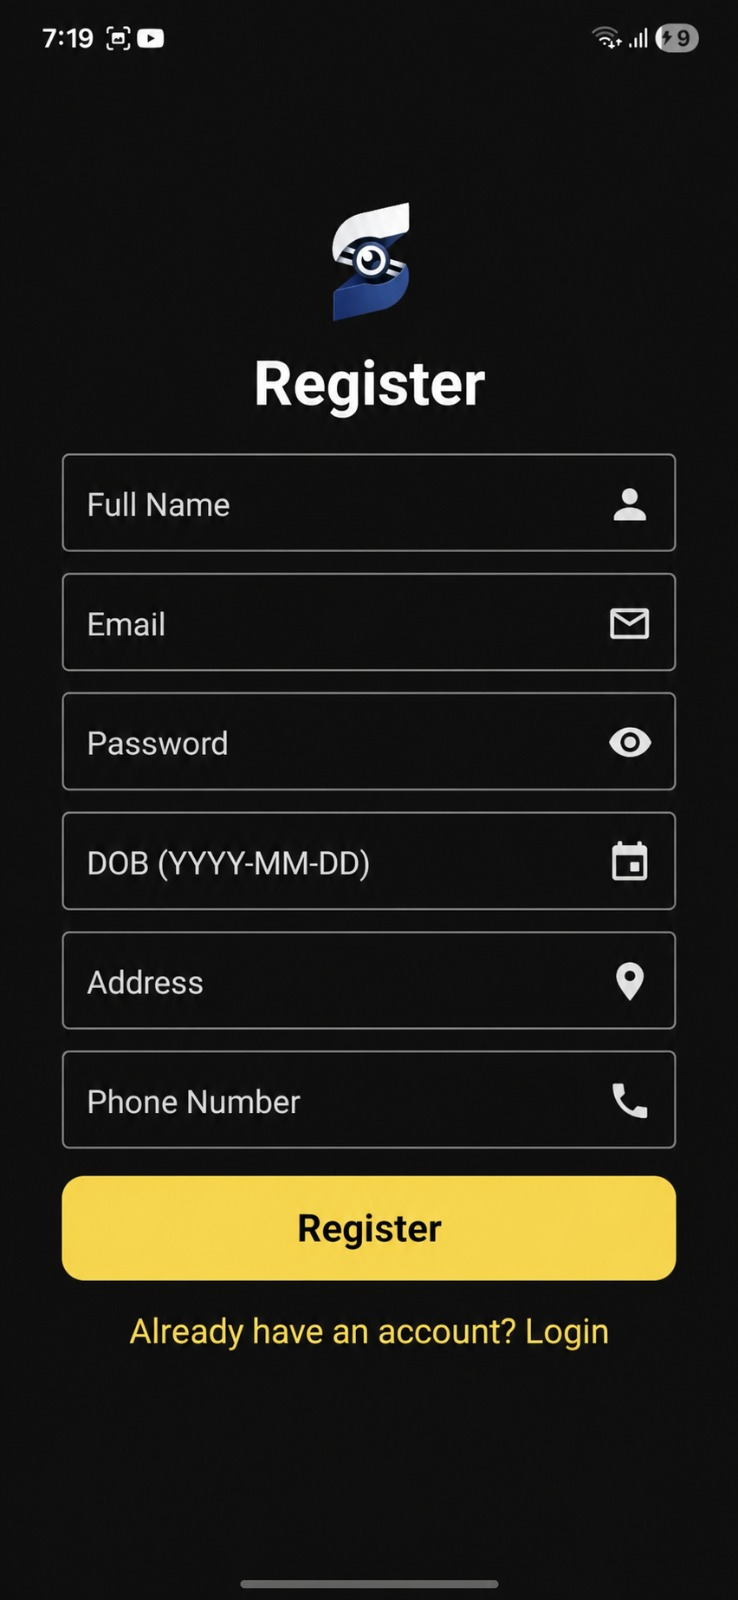
\includegraphics[height=0.65\textwidth]{Figures/GUI2.jpeg}
    \caption{User Registration Page\\}
    
    \label{fig:3}
\end{figure}

\begin{figure} [!h]
    \centering
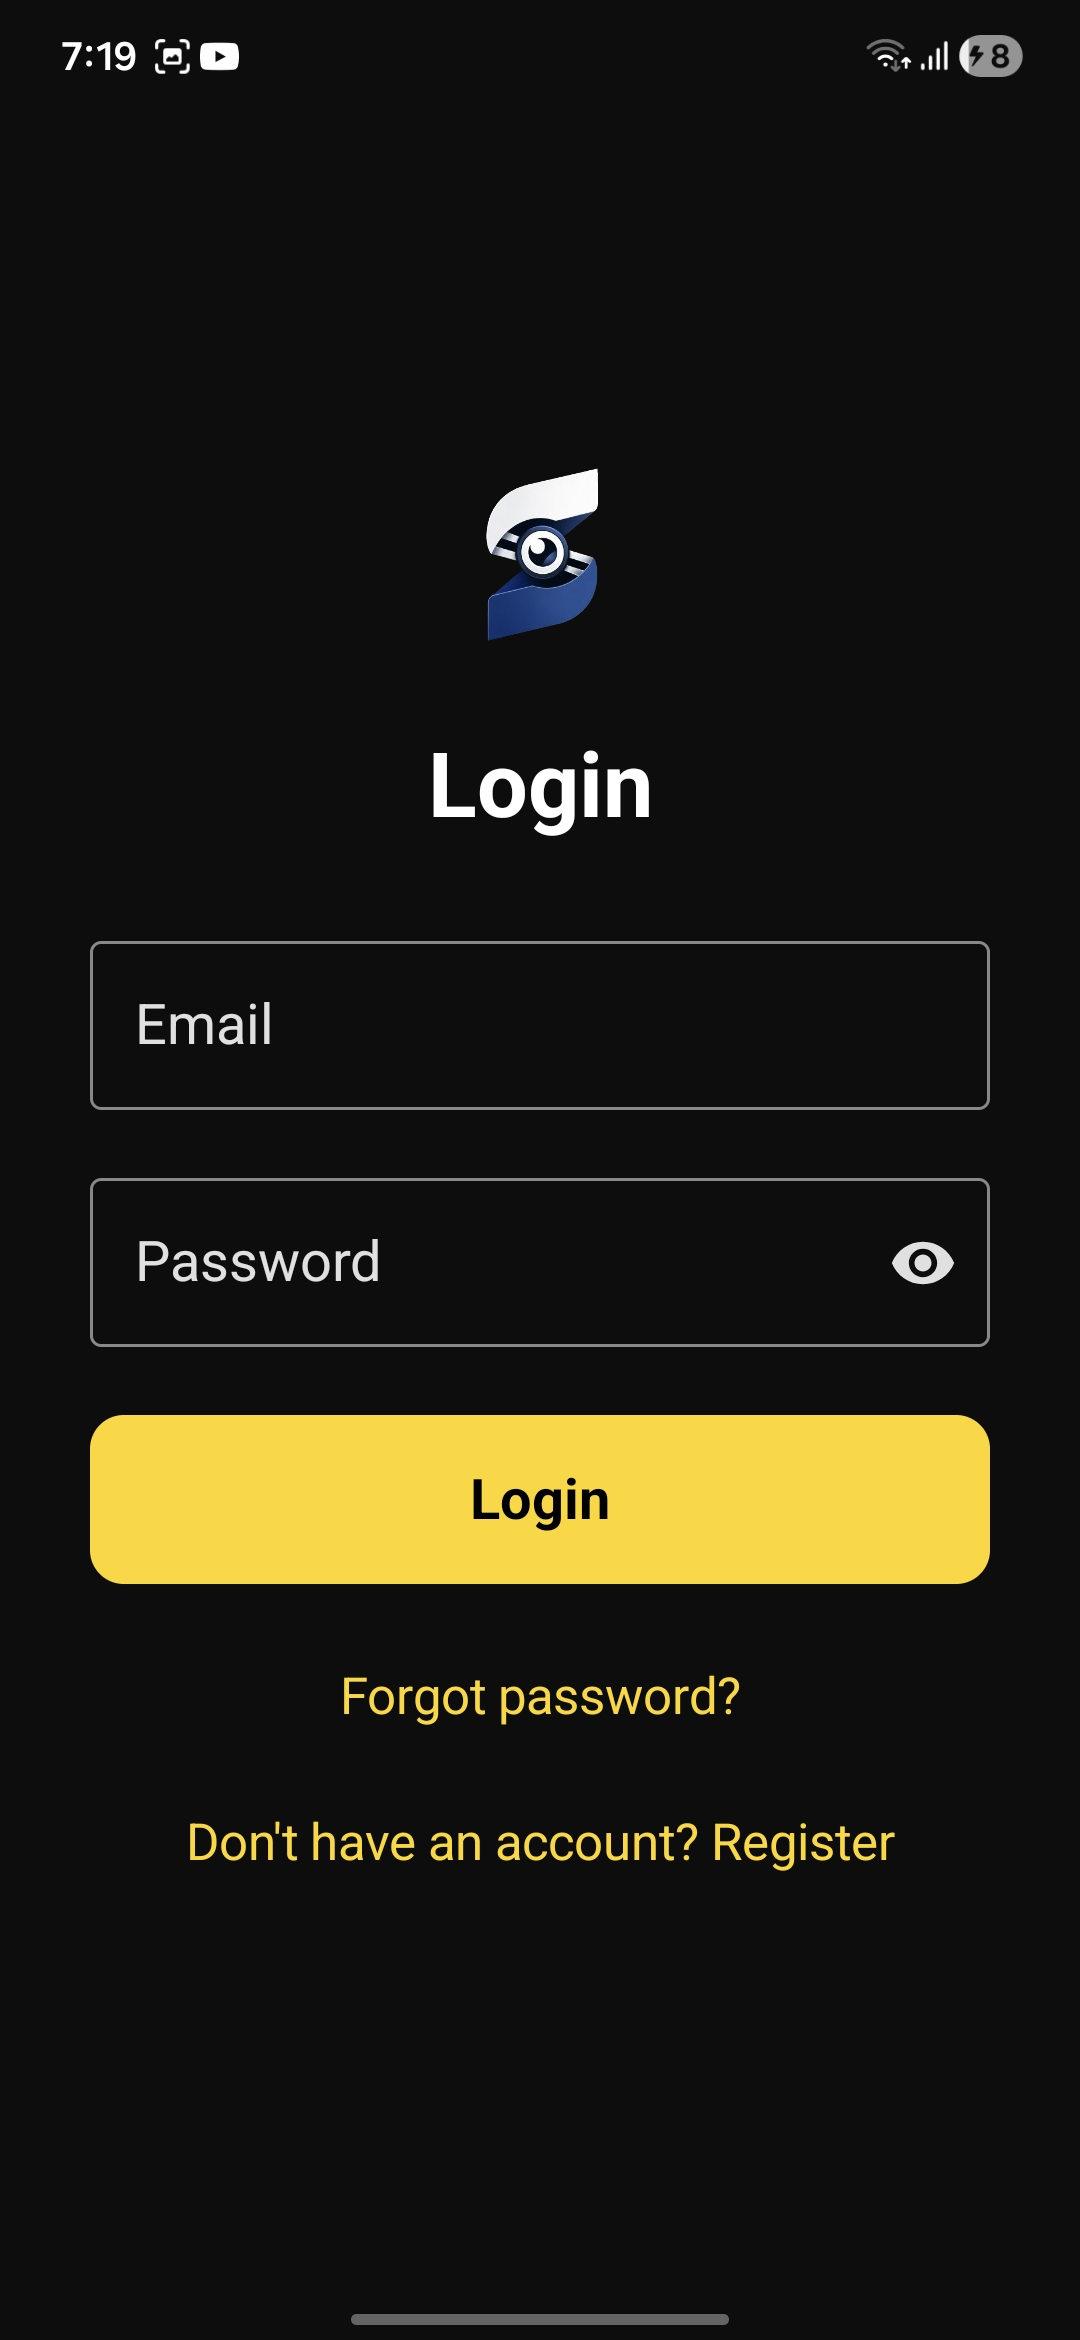
\includegraphics[height=0.65\textwidth]{Figures/GUI1.jpeg}
    \caption{User Login Page\\}
    \label{fig:4}
\end{figure}

\begin{figure} [!h]
    \centering
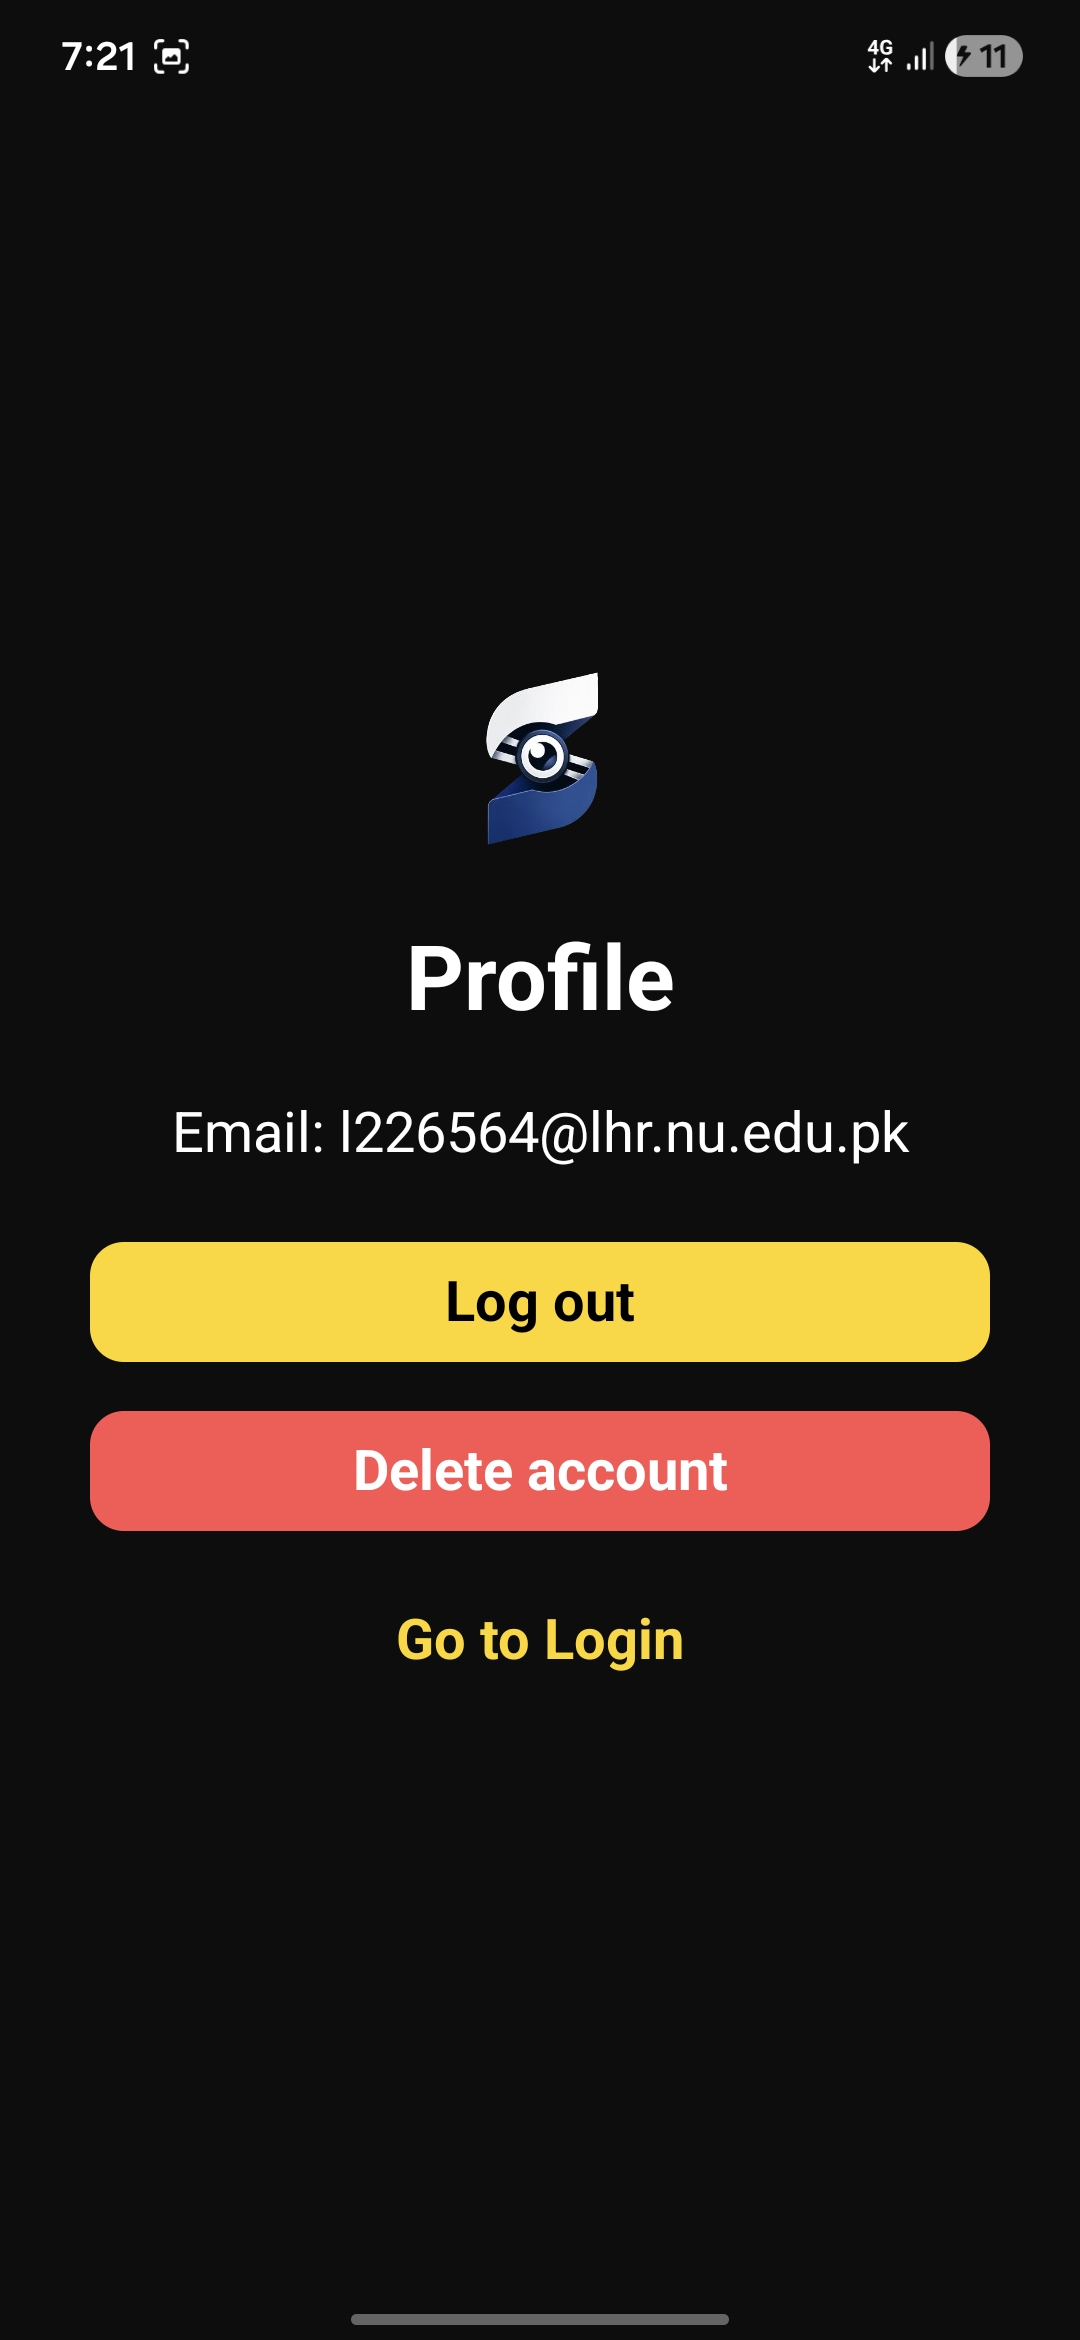
\includegraphics[height=0.65\textwidth]{Figures/GUI3.jpeg}
    \caption{User Profile Page\\}
    
    \label{fig:3}
\end{figure}

\begin{figure} [!h]
    \centering
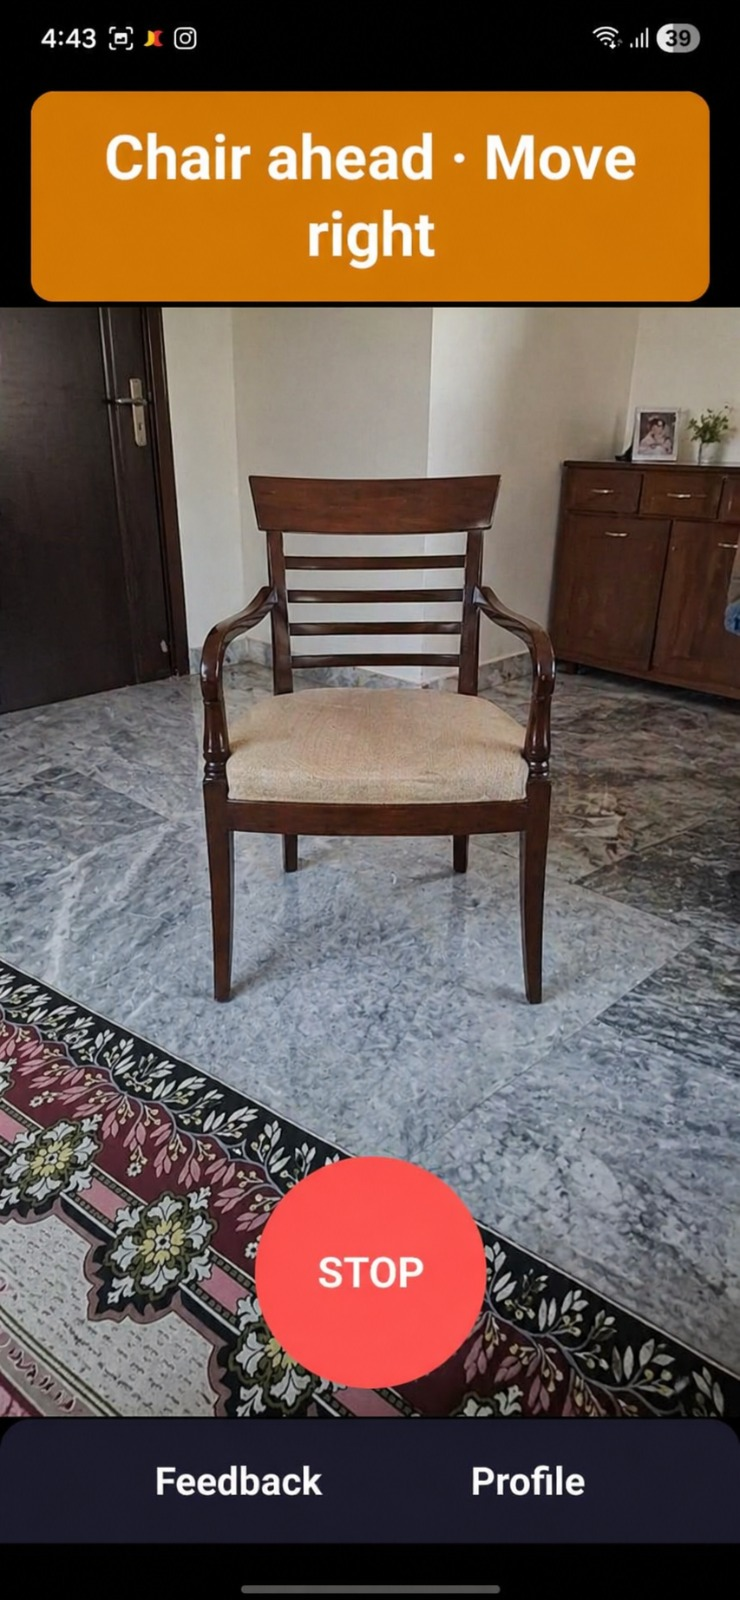
\includegraphics[height=0.65\textwidth]{Figures/GUI4.jpeg}
    \caption{Navigation Page\\}
    \label{fig:4}
\end{figure}

\begin{figure} [!h]
    \centering
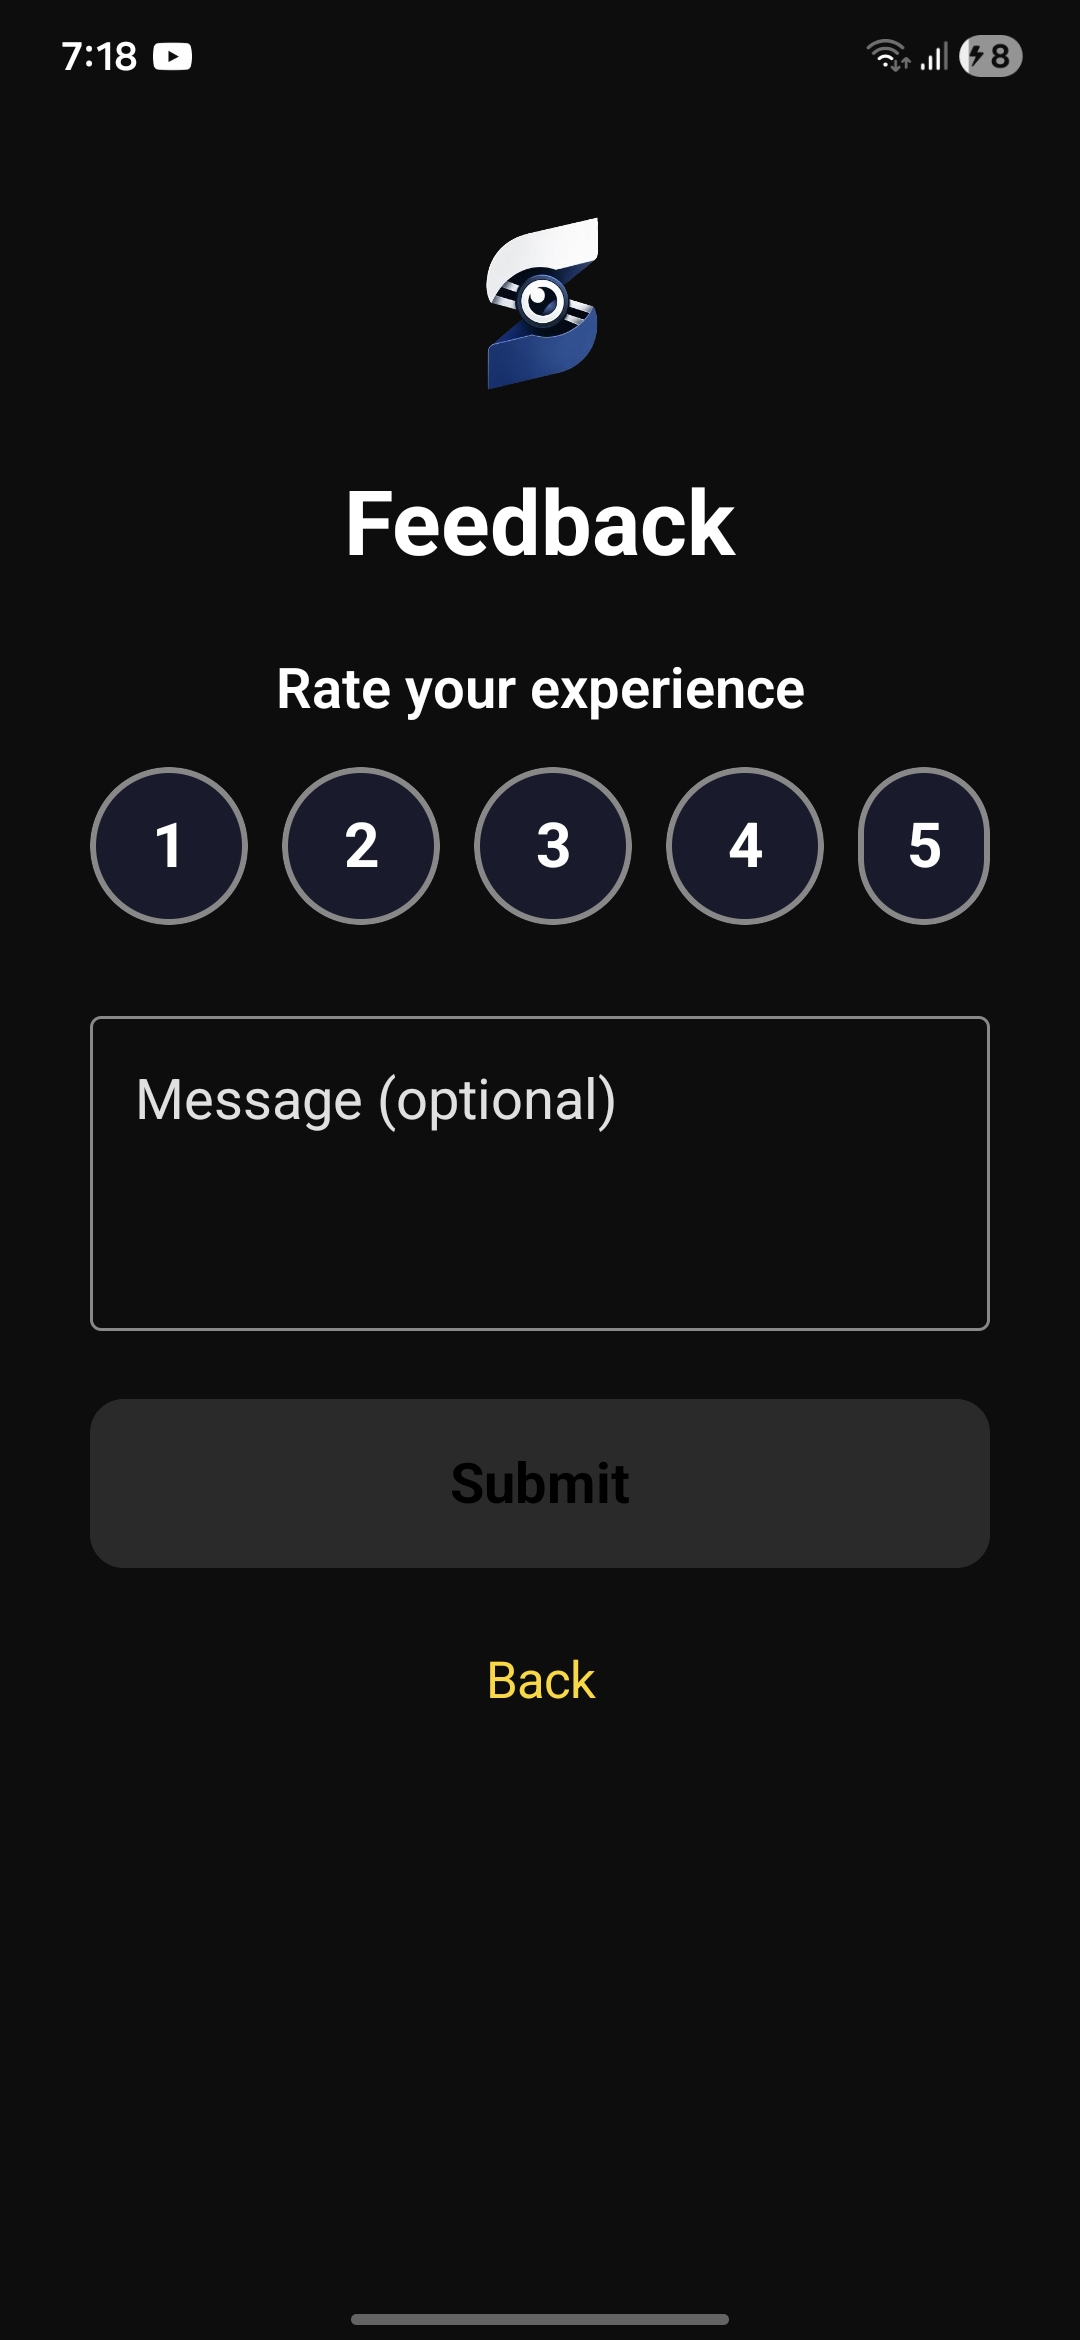
\includegraphics[height=0.64\textwidth]{Figures/GUI5.jpeg}
    \caption{Feedback Page\\}
    \label{fig:5}
\end{figure}

\pagebreak

\section{Database Design}
The schema used in our database is highly modular. User's information will be stored in the user table. Contact information table has been separated for security. Login information will be securely saved in the authentication table. Finally, the user feedback and ratings will be saved in the feedback table.

\subsection{ER Diagram}

    \begin{figure} [!h]
        \centering
    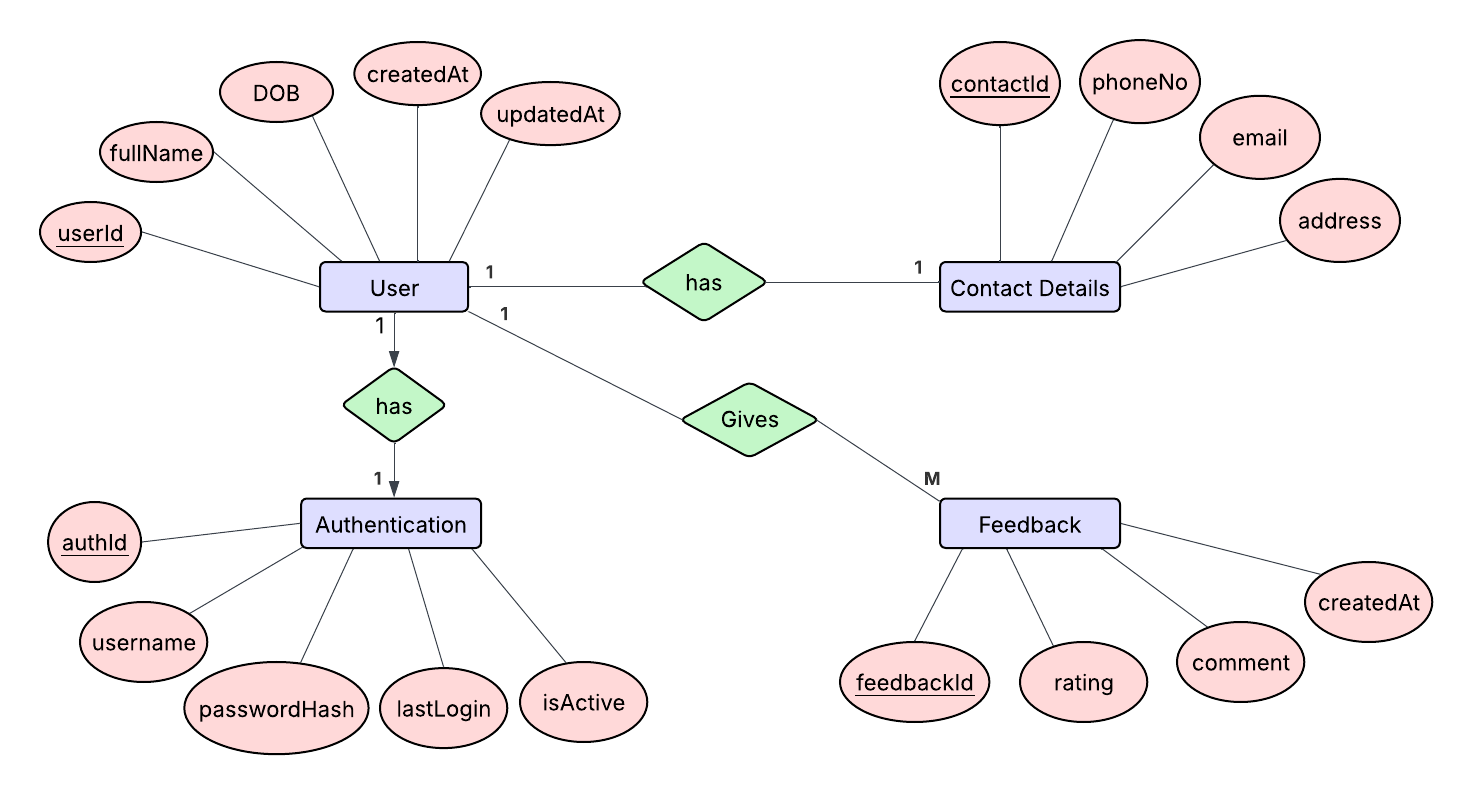
\includegraphics[height=0.44\textwidth]{Figures/erd.png}
        \caption{Entity Relationship Diagram\\}
        \label{fig:6}
    \end{figure}

\subsection{Data Dictionary}
\begin{table}[h!]
\centering
\caption{Data Dictionary}
\begin{tabular}{|c|c|c|c|c|c|}
\hline
\textbf{Entity} & \textbf{Attribute} & \textbf{Data Type} & \textbf{Relation To} & \textbf{Nullable} & \textbf{Description} \\
\hline
User & "userId" & int & & No & Unique ID (PK) \\
\hline
 & fullName & string & & No & Name of User \\
\hline
 & DOB & Date & & No & Date of Birth \\
\hline
 & createdAt & Date & & No & Date of User creation \\
\hline
 & updatedAt & Date & & No & Date of last Update \\
\hline
ContactDetails & "contactId" & int & & No & Unique ID (PK) \\
\hline
 & userId & int & User & No & corresponding User \\
\hline
 & phoneNo & string & & No & phone number of User \\
\hline
 & email & string & & No & email of User \\
\hline
 & address & string & & Yes & address of User\\
\hline
Authentication & "authId" & int & & No & Unique Id (PK)\\
\hline
 & userId & int & User & No & corresponding User \\
\hline
 & username & string & & No & username of User \\
\hline
 & passwordHash & string & & No & Hashed password of User \\
\hline
 & lastLogin & string & & No & When User last Logged in \\
\hline
 & isActive & boolean & & No & Is the User active \\
\hline
Feedback & feedbackId & int & & No & Unique ID (PK) \\
\hline
 & userId & int & User & No & corresponding User \\
\hline
 & rating & int & & No & Rating given by User \\
\hline
 & comment & string & & Yes & Comment about the experience \\
\hline
 & createdAt & Date & & No & When was Feedback created \\
\hline
\end{tabular}
\end{table}

\section{Risk Analysis}
The identification of risks and uncertainties that might affect the project execution is an important step in the process of planning a project. The purpose of risk assessment for our system is to look into many factors so that we can effectively mitigate any arising issues that might affect the successful delivery of the project.

\begin{itemize}
    \item \textbf{Hardware Failures:} While the software demands less hardware, certain unpredictable hardware malfunctions (such as camera problems, faulty speakers, and vibration motor failure) can pose challenges to availability of services. Regular maintenance of hardware and backup notification systems are therefore advised in order to address this challenge such that users get timely notification in case there is any problem with the hardware.
    
    \item \textbf{Software Compatibility:} The requirement of the application is that it uses the latest versions of the operating systems for mobile devices (Android). The functions like using a camera, playing audio, or background services might not work because of the non-compatibility or outdated versions.
     
    \item \textbf{User Experience:} The target users in this case are visually impaired people, therefore, accessibility is, the most crucial aspect. Usability can considerably reduce due to complicated or illogical interfaces. A simple audio-sound-based design with vibrotactile feedback will eliminate the risk by ensuring users receive clear and consistent instruction without any kind of visual interaction.
\end{itemize}

\section{Conclusion}
The aim of this chapter was to formalize the functional and non-functional requirements that will set a basis for developing Sighteo. System features, performance expectations, hardware and software needs, and quality attributes make the application reliable, usable, and safe for visually impaired users. This chapter translates the users' needs into structured requirements and hence provides an exact blueprint for subsequent design and implementation phases in such a way that each component of the system is aligned with the core purpose of the project.


\chapter{Proposed Approach and Methodology}
This chapter sets out the general approach informing the design of our assistive navigation system, Sighteo. The structure of the software itself, the selection of the central models employed, and their integration process, as well as the influence of users' feedback on every design choice, is explained in the description above. The subsequent paragraphs describe the methodology behind the project, its ethical approach, and its future development paths.

\section{Overview of the Proposed Approach}
Developing an application for a mobile device, which will assist blind individuals in navigating their surroundings using the camera of the phone only, without resorting to additional technologies such as LiDAR or GPS, is the ultimate aim. Our system focuses on accessibility and affordability by making use of computer vision (CV) models running on the backend. Real-time video frames, captured by the smartphone camera, are sent to the backend for processing. The backend processes the input frame by making use of object detection and vision-language models, then sends audio and haptic feedback to the user. 

\section{Methodology}
Iterative model development combined with software engineering best practices is the methodology adopted for this project's development. Our approach comprises of following phases:  

\begin{enumerate}
    \item \textbf{Requirement Analysis and Data Collection:} Datasets comprising of annotated objects (doors, stairs, obstacles, furniture) present in an indoor environment must be collected. Interviewing with visually impaired users and accessibility experts can help in defining user-centric requirements.  

    \item \textbf{Preprocessing and Model Selection:} Input data for object detection must be preprocessed alongwith semantic segmentation tasks. A suitable pre-trained vision-language model such as YOLO-based frameworks with depth estimation must be selected.  

    \item \textbf{System Architecture Design:} Mobile frontend developed using Kotlin, ensuring compatibility across Android. Backend implemented in Python for AI inference models.

    \item \textbf{Integration of Feedback Mechanisms:} Audio feedback by making use of text-to-speech modules to announce detected objects and provide verbal guidance. For urgent alerts like approaching obstacles, non-verbal cues will be given like beeps and vibration patterns.

    \item \textbf{Testing and Evaluation:} Volunteer test subjects can be employed for testing the system in a controlled indoor environment. Detection rate, response time, and user satisfaction ratings can be the test metrics. Based on test results, iterative optimization can be performed.
\end{enumerate}

\section{Agile Development}
Agile Development Approach to allow for incremental improvements and feedback from users will be followed. Our main markers are initial prototype, integration of object detection, testing of feedback mechanism, and usability tests, upon which sprints will be based. Flexibility and user-initiated changes are taken care of by Agile.

\section{Tools and Technologies}
\begin{itemize}
    \item \textbf{Frontend:} Kotlin  
    \item \textbf{Backend:} Python  
    \item \textbf{AI Models:} Pre-trained object detection models (e.g YOLO) with fine-tuning to support important obstacles like walls, stairs etc.  
    \item \textbf{Database:} PostgreSQL (or any other database service).
\end{itemize}

\section{Ethical and Accessibility Considerations}
A lot of focus is going to be placed on accessibility because the intended participants will be visually impaired persons. Following the requirements as per the WCAG guidelines, privacy protection of the images captured, and not providing unnecessary inputs on behalf of the user is part of this. Ethical considerations can be catered for by testing the system using actual participants.

\section{Future Directions}
Although the initial focus is on indoor navigation in controlled environments, our methodology will allow us to progressively extend the scope of our project in future. The project roadmap is as follows:
\begin{itemize}
    \item Semi-controlled indoor environments like navigating in buildings with moderate variations.
    \item Dynamic environments with moving objects and unpredictable layouts.  
    \item Outdoor navigation, incorporating distance-aware detection in unconstrained settings. 
\end{itemize}

\section{Conclusion}
In short, the methodology blends AI object detection and real-time feedback into a mobile application. It begins with the selection of a suitable base model from out of YOLOv8, SSD and RetinaNet. After selection, we'll move to fine tuning the model to the specific needs of the vusially impaired individuals. Scalability, affordability, and accessibility are offset in the project by the utilization of lightweight on-device computation managed with help of Python and Kotlin. Agile development model allows for iterative fine-tuning. Aim is to increase inclusivity and trust in the visually challenged community. This will be ensured through ethical guidelines.


\chapter{High-Level and Low-Level Design}
The following chapter describes the high-level and low-level design for Sighteo and explains how different components work together to support indoor navigation in real-time. This includes a high-level description of the major architectural choices, system modules, and the flow of data from the camera down to the feedback layer. The provided details form the technical backbone of the application. In this way, the chapter sets up the structure that will be needed during implementation in later phases.

\section{System Overview}
The system allows visually impaired people to navigate indoor environments safely and independently. The procedure includes system architecture designing, preparing and fine-tuning datasets, training the detection model, integrating the trained model into the mobile application, and providing audio and haptic feedback to the user.

\subsection{System Design}
Sighteo's system is organised into a set of interconnected modules that work together to deliver the final objectives of the application. Each module handles a specific part of our intended workflow. Following is a description of the composition of our system.

\subsubsection{User Authentication}
The authentication module is the point where users start their experience. It contains signup and login functionality to ensure secure access. This module validates users' credentials, and smoothly transitions them to the navigation interface.

\subsubsection{Navigation Control}
The navigation module is the core functionality of the application. It allows users to control when to start and when to stop navigation from the homepage. When navigation is activated, the trained AI model is the fed real time video frames from the camera, which provides navigational cues as the output.

\subsubsection{Object Detection and Feedback}
The object detection module processes the video frames from the camera using the AI model, which would be selected after ample experimentation and considering trade-off between accuracy and speed. The model identifies obstacles in real time, and the user is alerted through audio and haptic feedback.

\subsubsection{User Feedback}
This module provides users with an option to report any issues that they encounter using the application. A button will be provided on the homepage for this purpose. This will provide endless opportunities for application refinement.

\subsection{Data Collection}
For detection model training, datasets containing everyday objects present in a common indoor setting will be collected. Techniques for data augmentation like rotation, scaling, and brightness will be used for enhancing diversity and strength. These procedures ensure that the model will perform efficiently under varying environmental conditions such as varying light or object orientation.

\subsection{Model Training}
The training phase resolves around preparing the dataset collected for the detection model. The dataset is annotated with object classes for indoor navigation. The AI model will be trained and fine-tuned to provide a balance between detection and inference speed. Experimental comparisons would be conducted among different AI models and their respective variants to make sure that the chosen model is the most stable and reliable. The chosen model is then fine tuned and integrated into our application.

\section{Design Considerations}
This section includes some of the important issues that need to be addressed before Sighteo is designed: This can assist in highlighting several technical issues, user expectations, and environmental issues that might dictate the behavior of an app in actual practice. By analyzing such concerns at an early stage, the design should remain practical and scalable, and meet the needs of visually impaired users by ensuring that each and every design decision supports the requirements for safety, reliability, and consistency in navigation.

\subsection{Assumptions and Dependencies}
The design of Sighteo relies on the following assumptions and dependencies to ensure proper functioning:
\begin{itemize}
\item \textbf{Related software or hardware:} Smartphones would be not have outdate software, have functional cameras, speakers and vibration motors for feedback. 

\item \textbf{Operating systems:} The application would be compatible with Android.

\item \textbf{End-user characteristics:} The user would have the fundamental knowledge of how to use and operate a smartphone and the applications installed on it.

\item \textbf{Possible and/or probable changes in functionality:} The application considers the possibility of introducing newer object detection models in the future, or different ways of feedback to the user.

\end{itemize}


\subsection{General Constraints}
Sighteo's design is shaped by various constraints, each significantly impacts the system’s software architecture and functionality.

\begin{itemize}
    \item \textbf{Hardware or software environment:} Sighteo depends on mobile devices equipped with functional cameras and vibration hardware. Low-end devices may experience slower response times due to limited processing power or outdated hardware.
\item \textbf{End-user environment:} Object detection can be hindered due to usage in environments with poor lighting, cluttered spaces, or fast moving objects.
\item \textbf{Availability or volatility of resources:} The device's resources such as battery life, camera quality, and processing speed play a major part in system's performance. 
\item \textbf{Standards compliance:} The design must show compliance with accessibility standards for visually impaired individuals. It should also obey platform specific guidelines like Google play requirements.
\item \textbf{Interoperability requirements:} The application must work smoothly with the trained YOLOv8 model and mobile device hardware. Interoperability in the future could be expanded to cloud-based updates or third-party accessibility services.
\item \textbf{Interface/protocol requirements:} The user interface must be simple ensuring easy transition between the login, main page, and feedback page. Communication protocols between app modules like camera feed and feedback delivery etc should work efficiently in real time.

    \item \textbf{Data repository and distribution requirements:} User's information must be safely stored in an encrypted database. Data distribution, such as model updates, must go via secure channels to prevent security issues.
    \item \textbf{Security requirements (or other such regulations):} The system must protect sensitive information like login credentials from unauthorized access. Data in storage and transmission should be encrypted to avoid tampering.
    \item  \textbf{Memory and other capacity limitations:} Mobile devices with limited RAM or processing capacity may face difficulty in running the app efficiently and smoothly. Therefore, the size of the model must be optimized to reduce overloading the device.
    \item \textbf{Performance requirements:} The system must deliver real-time feedback. It should be able to target at least 15–20 frames per second for obstacle detection to ensure safe navigation with audio and haptic feedback.
    \item \textbf{Network communications:} Even though navigation process does not require internet, internet connectivity may be required for updates and feedback posting. These services could be delayed due to disruption in internet.
    \item \textbf{Verification and validation requirements (testing):} Testing will be performed in controlled environments to ensure detection accuracy, timely feedback, and system dependability prior to widespread deployment.
    \item \textbf{Other means of addressing quality goals:} Frequent user testing with visually impaired users will improve usability. Ongoing updates and patches will remedy bugs and enhance accuracy.
    \item \textbf{Other requirements described in the requirements specification:} Additional requirements may include multi-language support in the help system and scalability for integration with future external sensors or wearable devices. 
\end{itemize}
\subsection{Goals and Guidelines}

 

Sighteo is designed around a number of goals, directives, principles, and priorities for effectiveness, reliability, and user-friendliness of its design for visually impaired users. 

\begin{itemize}
    \item \textbf{The KISS principle ("Keep it simple stupid!"):} Sighteo adoption requires simplicity. Only essential functions like Start/Stop Navigation and Help are placed front and center on the home page. This minimizes complexity and allows users to use the app easily and confidently.  

    \item \textbf{Emphasis on speed versus memory use:} Sighteo is focused on low-latency performance. After experimentations and testing, YOLOv8 was selected due to the best blend of accuracy and speed.

    \item \textbf{Accessibility and user-centered design:} It is very important that the application must be as simple as possible with haptic feedback for accessibility. This will avoid users being confused with the interface.

    \item \textbf{Reliability and safety:} As a safety assistive tool, safety is of paramount importance. In order to make the users trust the application, design guidelines have been followed strictly to allow consistent and reliable detection and feedback.

    \item \textbf{Scalability and adaptability:} Currently, Sighteo is aimed for indoor navigation, but the development will done in such a way to integrate outdoor navigation in the future.
\end{itemize}

 
\subsection{ Development Methods}
The development of Sighteo follows a systematic and well-defined approach to ensure reliability, accessibility, and adaptability.  

\begin{itemize}
    \item \textbf{Agile Development Methodology:} Agile approach has been used in Sighteo to handle changing requirements and make the development stage more flexible. Work is divided into sprints, concentrating on modules like authentication, navigation control, and feedback mechanisms. The process ensures continuous improvement via incremental posting.

    \item \textbf{Iterative Design Process:} The system uses an iterative design cycle to improve core functionalities. Testing and feedback are taken into account in each iteration so that the navigation experience becomes more and more accurate, responsive, and user-friendly.

    \item \textbf{User-Centered Design (UCD):} Sighteo is built for visually impaired individuals, therefore, UCD principles are vital to its development. The highest priority has been given to feedback mechanisms, interface simplicity, and accessibility features such as haptic alerts as this ensures that the system aligns with the expectations and safety requirements of its target audience.
\end{itemize}


\section{System Architecture}
\begin{figure} [!h]
        \centering
    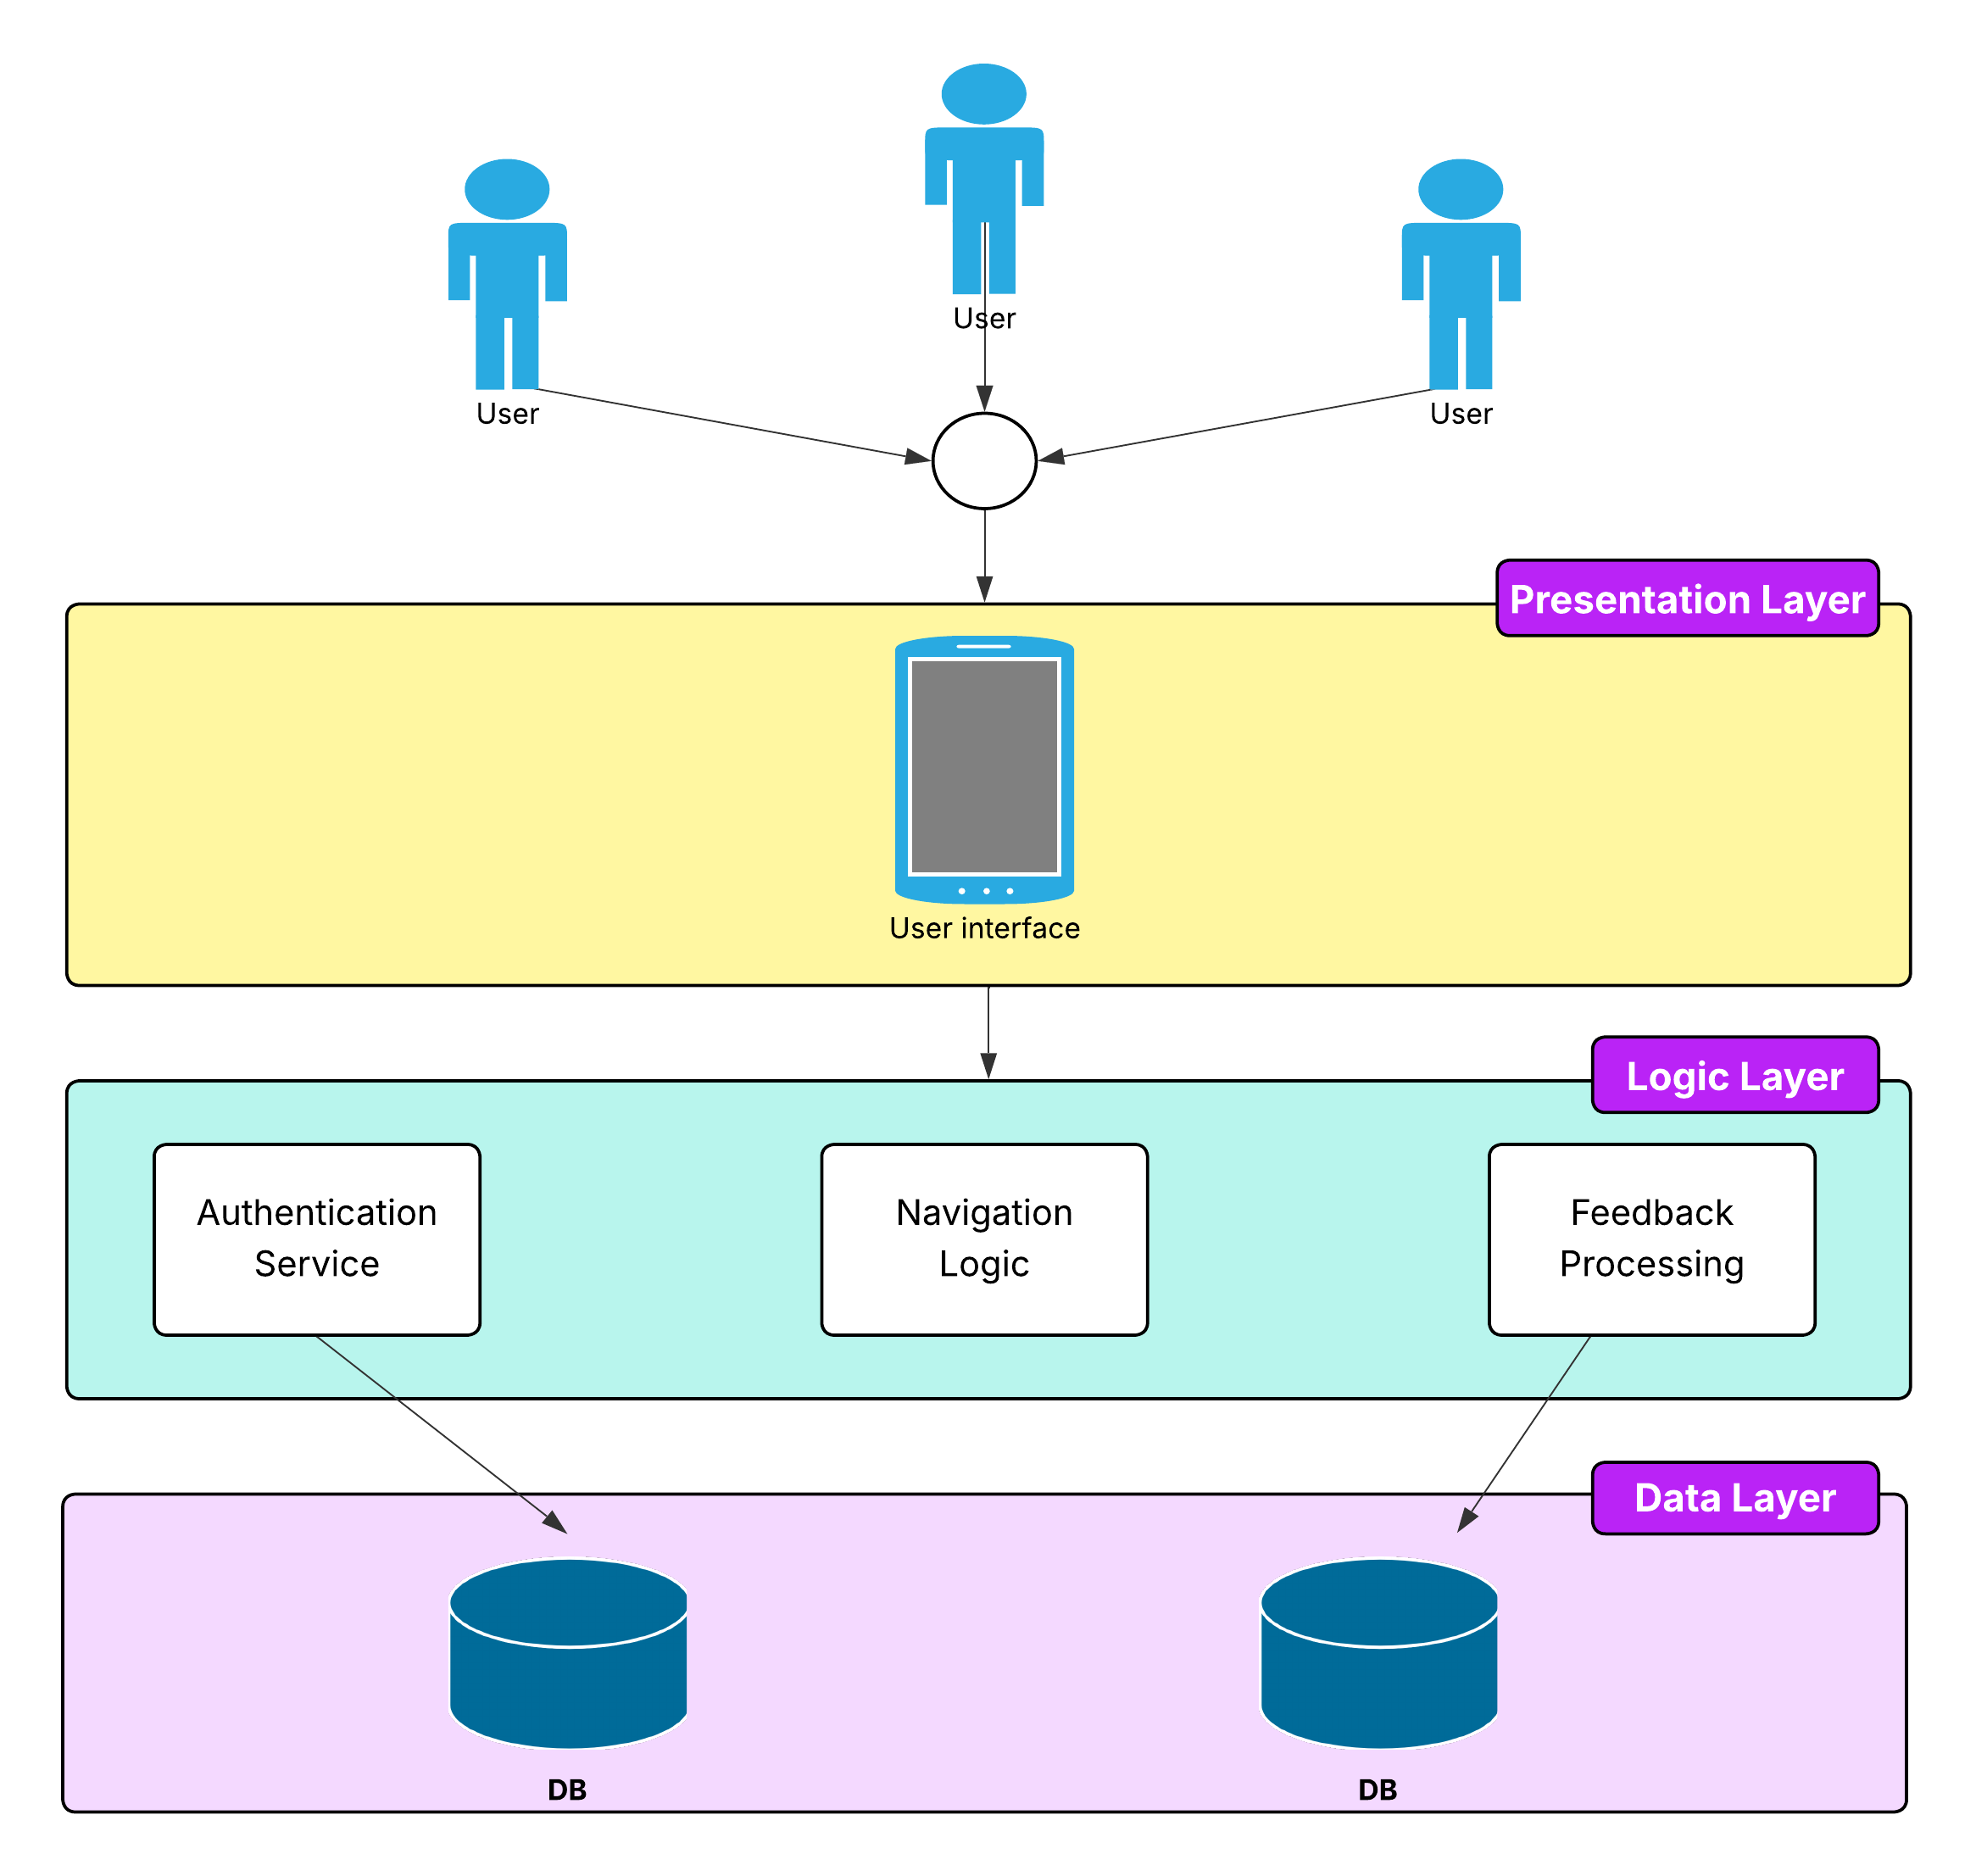
\includegraphics[height=0.60\textwidth]{Figures/highLevel.png}
        \caption{High Level System Architecture Diagram\\} 
        \label{fig:7}
    \end{figure}
System architecture includes three layers interacting with each other: presentation, logic, and data. In the presentation layer, there is a mobile app serving as an interface of the system. With its help, users' videos are captured using the camera, whereas the results from the processing are returned in the form of audio or vibration signals. This approach allows visually challenged people to react to the world around them better. The logic layer is where all processes of the system take place. It is here that video frames undergo further analysis using the obstacle detection algorithm and navigation logic. Thus, obstacles are detected, and the best route of movement is found by users. As for the data layer, it stores essential information about users, including their credentials and feedback. Therefore, safe access to the system becomes possible, and improvements of the process based on users' experience can be made.
\pagebreak
\subsection{Subsystem Architecture}
\begin{figure} [!h]
    \centering
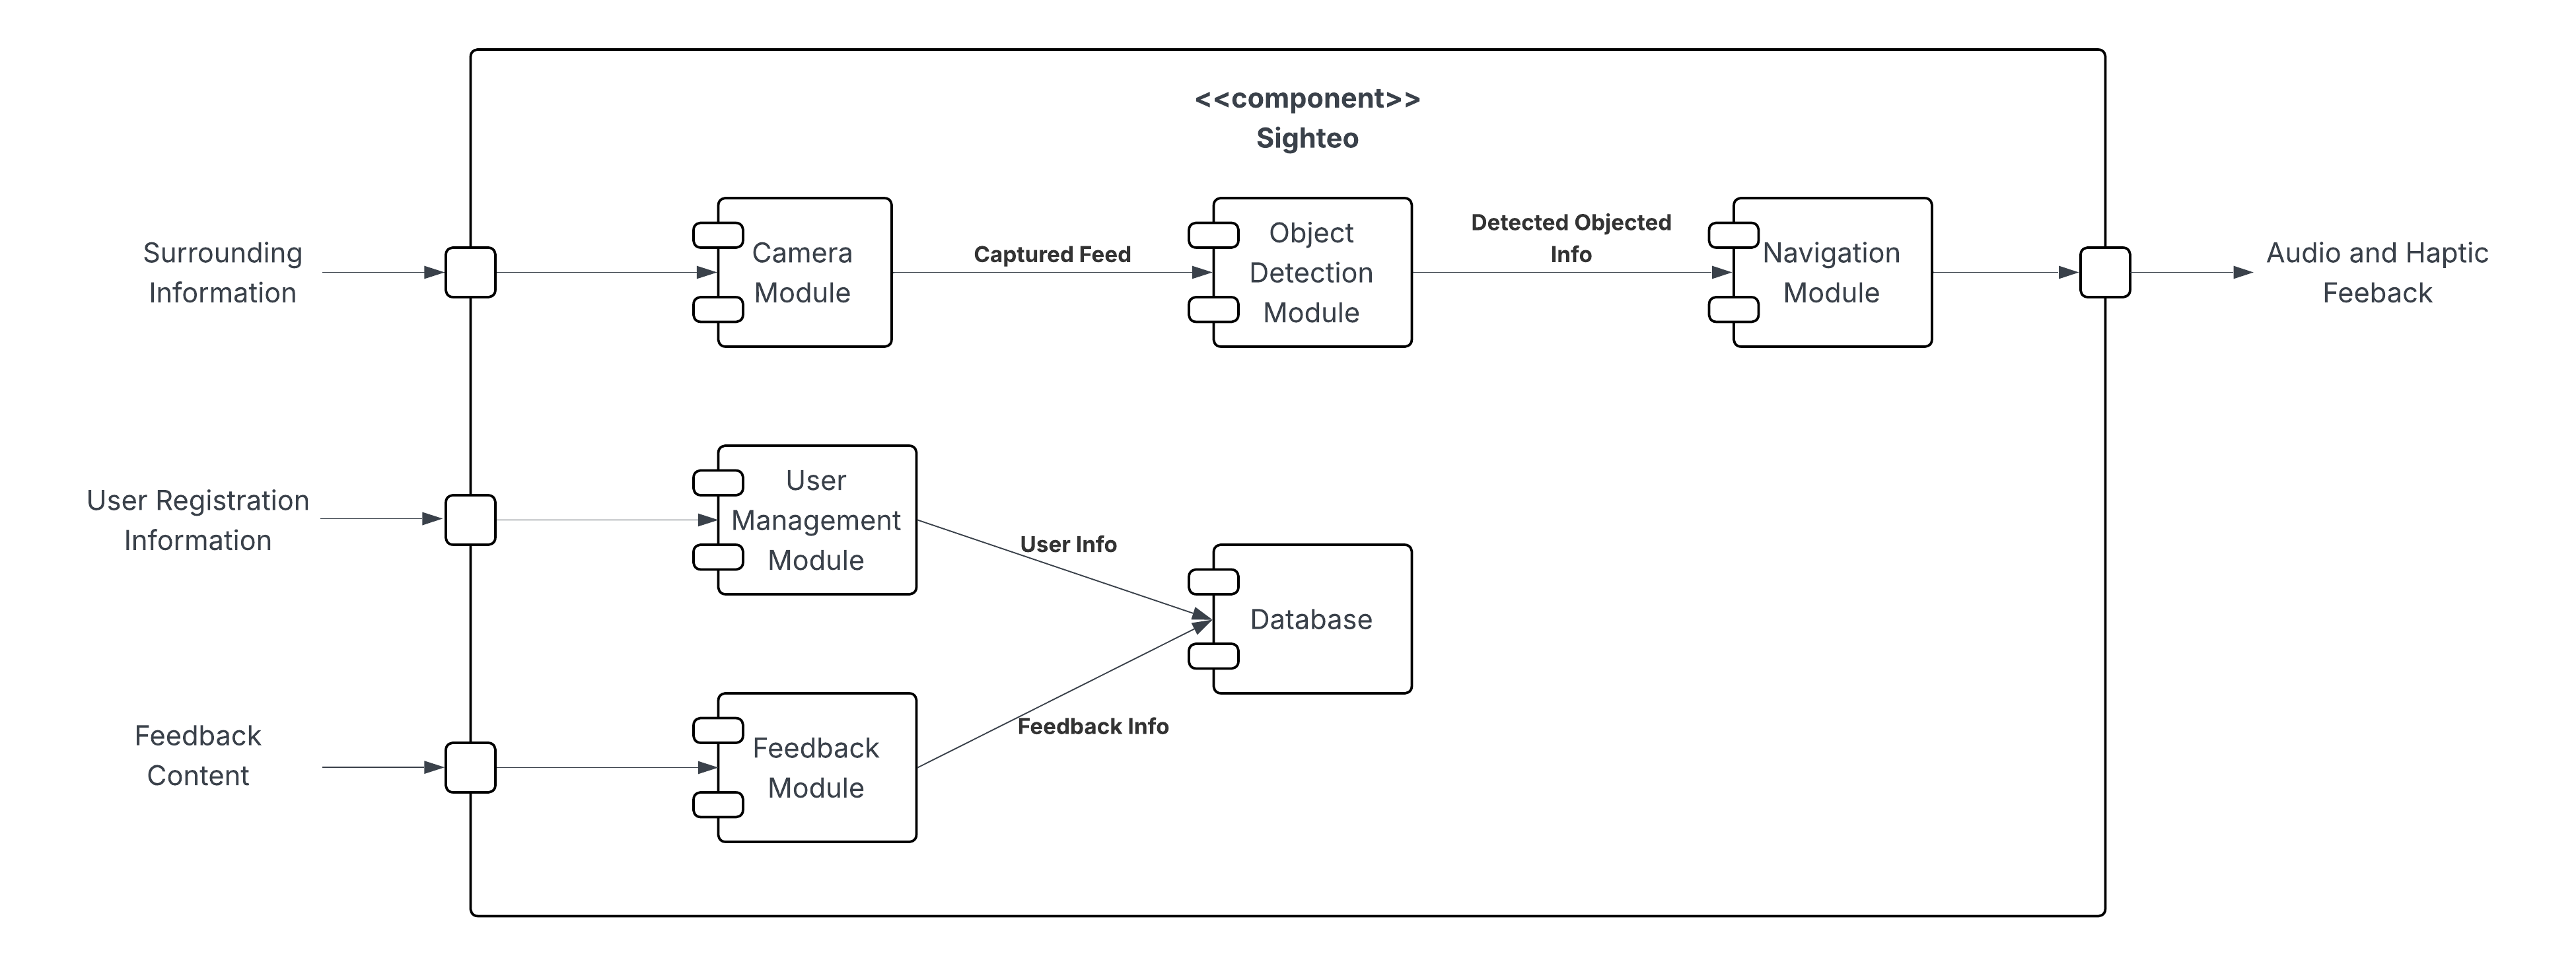
\includegraphics[height=0.38\textwidth]{Figures/Component.png}
    \caption{Sub-System Architecture Diagram\\}
    \label{fig:8}
\end{figure}
The Sighteo subsystem architecture is designed in such a way that the components interact with each other in order to enable navigation assistance. The first step is for the camera component to gather live video feed, and then pass the feed to the object detection component in the form of video feeds for obstacle detection. All this information is passed to the navigation component, which will determine the safest route and give feedback to the user using audio and tactile feedback. The User Management Component takes care of the authentication process and keeps all sensitive data stored in the database, while the feedback component keeps a record of users’ experiences.

\section{Architectural Strategies}
The architectural approaches for Sighteo application revolve around delivering reliable real-time support to users who have visual disabilities and setting up cross-platform compatibility, scalability, and robust security. The mobile application will be developed using Kotlin, whereas the entire backend will be designed in Python. This architecture ensures that the application is lightweight and responsive in the mobile environment, whereas the backend effectively handles AI processing and calculations.

\subsection{Tools and Software}
This portion discusses the technical foundation behind the ability of Sighteo to operate efficiently in real time. This includes the key software elements, hardware specifications, communications process, and security aspects that make up the whole system.

\subsubsection{Mobile Application:}
\begin{itemize}
  \item Developed using \textbf{Kotlin}, enabling compatibility with Android.
  \item Usage of device features like Text-to-Speech (TTS), vibration motor for feedback.
\end{itemize}

\subsubsection{Backend Services:}
\begin{itemize}
  \item Implemented in \textbf{Python} to gain access to newer and better libraries and packages
  \item Machine Learning using TensorFlow.
  \item Middleware layer for request handling and load balancing.
\end{itemize}

\subsubsection{Communication Protocols:}
\begin{itemize}
  \item Lightweight payloads like JSON or protobuf carry detection outputs such as object type, relative distance, and confidence scores.
\end{itemize}

\subsection{Hardware}
\textbf{Client Devices:} Smartphones with a working rear camera and vibration motor.

\subsection{Communication Mechanisms}
\begin{itemize}
  \item The mobile client captures video frames at a preset rate based and sends them securely to the backend.
  \item The backend processes the frames, performs inference, and sends back results for instant playback.
\end{itemize}

\subsection{Error Detection and Recovery}
\begin{itemize}
  \item Backend implements retry mechanisms in case of internal errors.
  \item Uncertainty within model detection is communicated conservatively (e.g., ``possible obstacle ahead'') instead of remaining silent.
\end{itemize}

\subsection{Security and Data Privacy}
\begin{itemize}
  \item All API calls will be secured by secrets.
  \item No video frames are permanently stored on the backend as results are delivered in real-time.
\end{itemize}

\subsection{Future Plans}
\begin{itemize}
  \item Integrate traffic signal recognition, obstacle trajectory prediction, etc in the future.
  \item Enhance multi-language voice support to better serve diverse user groups.
\end{itemize}



\section{Domain Model/Class Diagram}

\begin{figure} [!h]
    \centering
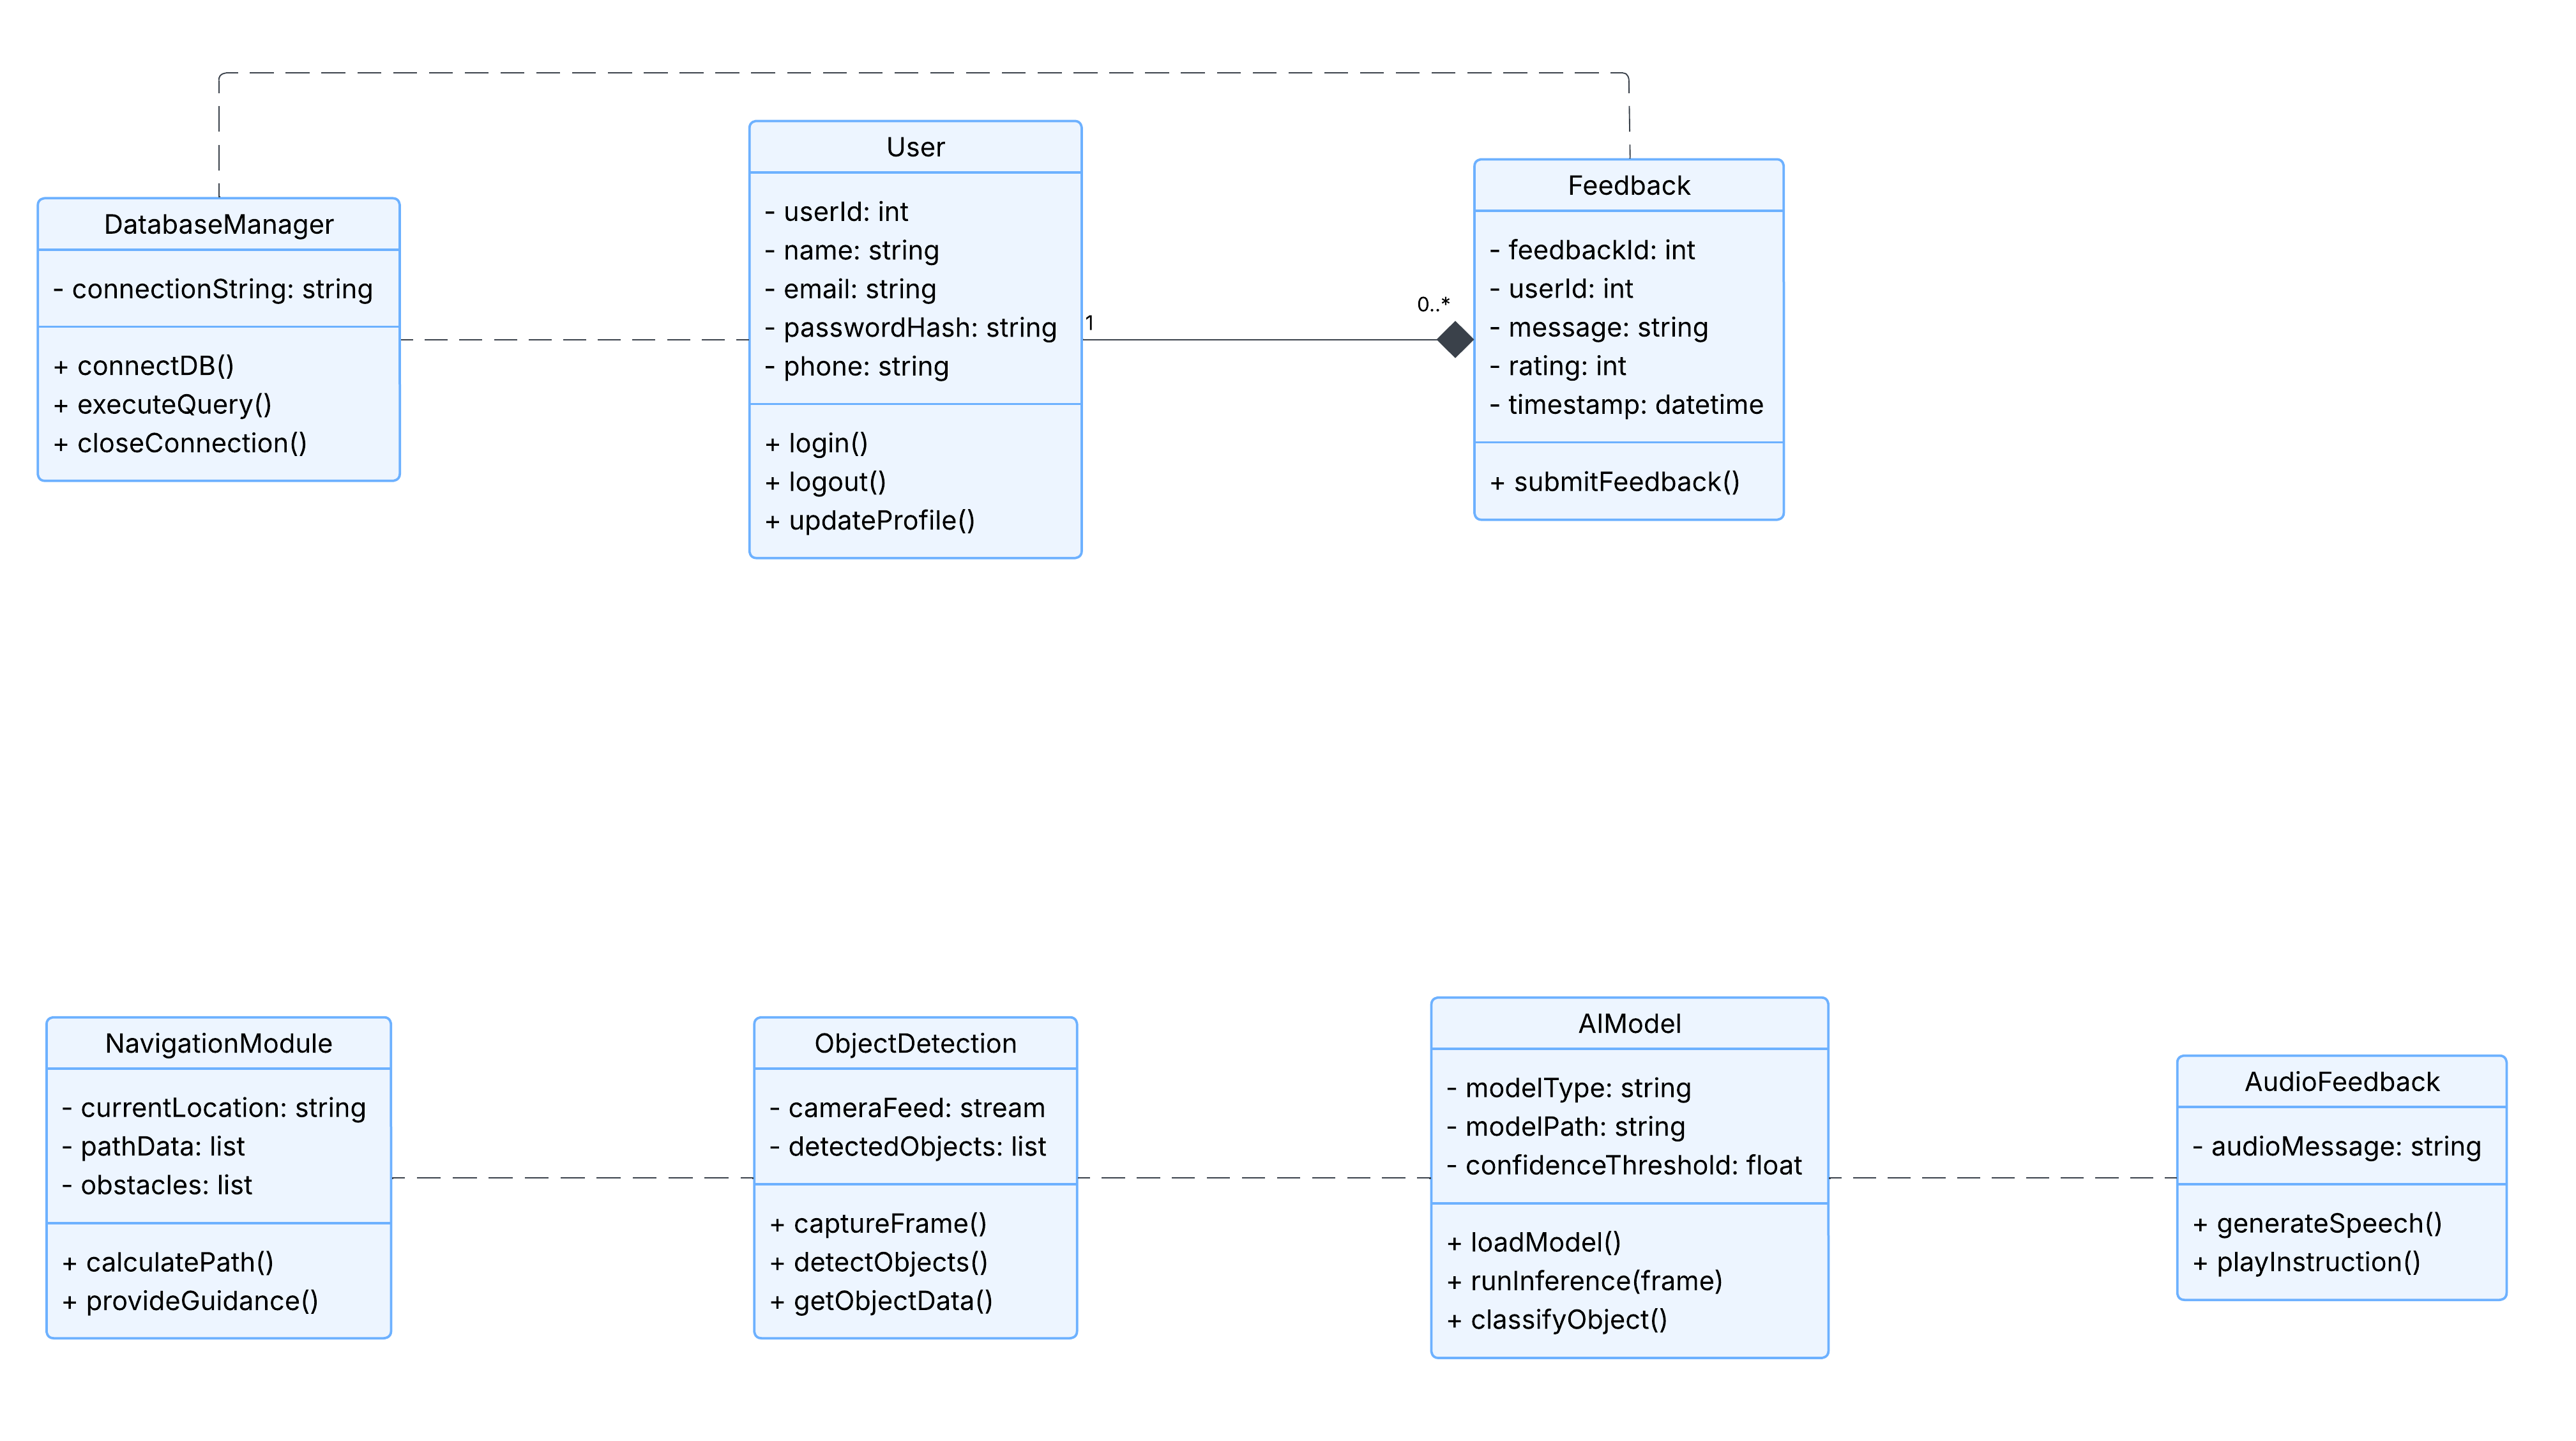
\includegraphics[height=0.5\textwidth]{Figures/classDiagram.png}
    \caption{Class Diagram\\}
    \label{fig:9}
\end{figure}

\section{Policies and Tactics}
The policies and strategies adopted while designing Sighteo are elaborated upon in this section. While these factors do not play an important role at the architectural level of the system, they definitely influence other aspects of its implementation.

\subsection{Conventions and Coding Guidelines}
The development of Sighteo should conform to certain coding guidelines to make the code readable, consistent, and maintainable. Kotlin will be used for the mobile application. However, the backend and modeling will require the use of Python. There will be proper indentations in the code along with module coding guidelines and commentaries explaining certain procedures and methods. This will help other developers understand the code easily.

\subsection{Coding Environment}
The primary Integrated Development Environment (IDE) will be Visual Studio Code due to its extensive support for Kotlin and Python. It has built-in debugging tools, syntax hints, and extensions for version control like github. Furthermore, to manage Python environments during model training and experimentation, Anaconda will be used.  

\subsection{System Testing}
White-box and black-box test methodologies will both be employed in order to ensure the reliability of the system. Black-box testing will be used to test user interactions such as signin/signup, control navigation, and reaction to feedback, while white-box testing will ensure that modules like frame processing and YOLOv8 inference are correct. Unit tests and integration tests will be executed before deployment.

\subsection{Maintenance of Software}
Once the project is complete, bug fixes, dependency upgrades, and added features like support for semi-controlled outdoor spaces will be part of maintenance. Modular design will make it possible to update without halting the whole system.

\subsection{Extensibility}
Sighteo is extensible. The coding structure is modularized in nature, which facilitates the easy inclusion of new object recognition models or even sensors in the coming days. It enables this system to grow and develop further as technology advances.

\subsection{Engineering Trade-offs}
It has been programmed using a modular approach where any new algorithm or module may be easily integrated by future coders. It becomes easy in this manner for the program to evolve along with advancements in technology and user needs. One of the key design choices that had to be made in the design of the program was selecting YOLOv8 instead of the latest available such as YOLOv10. While the latest versions might give better results, YOLOv8 was selected because of its proven record of performance speed and stability.

\subsection{Requirements Traceability}
In order to make sure that everything is covered, there will be a relationship established between functional requirements and the modules developed. This will serve to ensure that all user requirements and objectives of the system have been completely fulfilled.

\subsection{Deliverables and Build Process}
Deliverables of the system will be the app for Android and the training of YOLOv8 model. Build activities will comprise the compilation of Kotlin codes and the connection of the application to backend services.

\section{Conclusion}
The deliverables from this project will include the mobile application for android operating system as well as the trained model of the YOLOv8 algorithm. The process of development includes compilation of Kotlin code and linkage with the back-end services. An introduction to the architecture, interactions between subsystems, design concepts, and technologies used to develop Sighteo system was made. Further on, more information about working of the application was provided. This chapter has established that the system is based on a scalable, maintainable, and user-centered foundation by identifying assumptions, constraints, and the ways in which it has been developed. It is these types of design decisions that provide the backbone for the implementation work continuing in successive chapters.

\chapter{Implementation and Test Cases}
Work done in terms of implementation of the application has been described in this chapter, including technical details and test cases which are not discussed in the high and low-level design.
\section{Implementation}

The implementation phase contained two main components. Firstly, a methodical model selection and fine-tuning process was undertaken. Secondly, the finalized model was integrated in an intuitive and functional Kotlin mobile application for real time navigation assistance.

\subsection{Model Selection and Fine-Tuning}

This phase was devoted to the identification and optimization of an object detection architecture that can achieve real time indoor obstacle detection on mobile hardware.


\subsubsection{Model Exploration}

Object detection architectures such as YOLOv8, SSD, and RetinaNet, which are currently considered to be the best in their class, have been taken into consideration. Object detection architectures that have been considered for evaluation are based on their ability to perform well in real-time object detection. All three object detection architectures have been considered for evaluation in terms of their detection accuracy, speed, and complexity. Special consideration needs to be given to the frame rates in the case of real-time, especially in the context of walking, as it affects the safety of the end users. The frame rates have a direct impact on the safety of the end users. YOLOv8 has been found to be the best in terms of accuracy and speed, as deduced from the preliminary benchmark.

\subsubsection{Dataset Selection and Preparation}

For the inspection and exploration of the object detection architectures, the commonly used COCO and Open Images datasets have been taken into consideration. It is to be noted that as the object detection architectures are to be utilized in the context of indoor environments, a filter has been added to the dataset to include only the relevant classes of objects.

\subsubsection{Evaluation Metrics}

To compare models in an objective way the following several metrics were used. The most important ones are stated below:

\begin{itemize}
    \item \textbf{Mean Average Precision (mAP):} Measures the quality of detection for the different classes of objects.
    \item \textbf{Frames Per Second (FPS):} Measures the performance capability in real time.
    \item \textbf{Model Size and Memory Consumption:} Measures the feasibility for mobile deployment
    \item \textbf{Latency and Power Consumption:} Measures responsiveness and resource efficiency
\end{itemize}

The general goal was to identify a model that maintained high detection accuracy and ensured real-time usability and efficient use of resources.

\subsubsection{Platform and Experimental Setup}

All the experiments were performed using Python based deep learning frameworks. Model benchmarking and visualization was performed with general machine learning libraries. Training and evaluation were conducted using a workstation with an Nvidia RTX 3060 GPU, and therefore consistent testing conditions were achieved across all the architectures.

\subsubsection{Final Model Choice and Fine-Tuning}

Following the methodology of comparative analysis, YOLOv8 was selected as the final architecture, which is attributed to the stable frame rate, small model size, and strong performance in different indoor lighting conditions. Subsequently, the model has been fine-tuned on the filtered indoor data set to improve the detection performance for the classes relevant for navigation. Hyperparameters were adjusted in an iterative manner to optimize convergence, detection accuracy, and inference stability.


\subsection{Mobile Application Integration}

After optimizing the model, the trained model (YOLOv8) was integrated into a Kotlin mobile application designed for visually impaired people.

\subsubsection{Model Deployment}

The trained model was converted to a mobile compatible tflite format to make it easier to perform on-device inference. This conversion removed the need for cloud processing and therefore reduced the latency and increased the reliability in environments with limited connectivity.

\subsubsection{Real-Time Detection Pipeline}

The mobile application captured the frames from the camera continuously and these frames were sent to the embedded object detection model. Bounding boxes of detected objects in each frame were analysed to determine relative positioning and possible risk of collision. A light weight layer of rules based logic gave priority to the obstacles that were most dangerous.

\subsubsection{Feedback Translation Layer}

Output from the detection pipeline was converted into actionable advice. Audio provided name of object and directional context. Haptic vibrations indicated start, stop, left and right. Vibrations are a better way to alert user as they will always be more prompt in informing user compared to a phrase or sentence being said to its full length. 


\subsubsection{End-to-End Testing}

Integrated system testing was carried out in controlled indoor settings, comprising of corridors and rooms with obstacles. Performance was measured from detections, response latency and clarity of user feedback. Observations from testing led to iterative refinements in both our fine tuned model as well as the mobile application. 

\section{Test Case Design and Description}

To test functionality of our application Sighteo, a series of test cases were designed. They aimed at testing our complete system in controlled indoor environments. Sighteo aims at helping visually impaired individuals therefore the test cases were carefully designed as per the specific needs of our end users.

All tests were run on Android mobile devices with an operational camera, speaker, vibratory support, and adequate processor. The tests were conducted in an indoor environment, such as corridors, classrooms, rooms, and hallways, under normal lighting conditions, unless otherwise specified. For the tests related to navigation, it was assumed that the application had been installed properly, the necessary permissions had been granted, and that the user had already activated the navigation module.

The test cases have common attributes, i.e. valid user interaction with the mobile interface, correct loading of the camera feed, correct initialization of the detection model, and successful activation of the output modalities such as audio and vibration. The running of any individual test case is usually independent of any others, except where there is a prerequisite such as logging in or permission approval. The following test cases were created in order to check the main features implemented in Sighteo.

\begin{table}[!ht]
\caption{User Registration}
\centering
\small
\begin{tabular}{|p{3.2cm}|p{3.3cm}|p{3.2cm}|p{3.3cm}|}
\hline
\multicolumn{4}{|c|}{\textbf{Authentication Module}} \\ \hline
\multicolumn{4}{|c|}{\textbf{Sighteo Mobile Application}} \\ \hline
\textbf{Test Case ID:} & TC-01 & \textbf{QA Test Engineer:} & Hasnain Khurram \\ \hline
\textbf{Test Case Version:} & 1.0 & \textbf{Reviewed By:} & Farooq Haider \\ \hline
\textbf{Test Date:} & 11/02/2026 &
  \multicolumn{1}{l|}{\textbf{\begin{tabular}[c]{@{}l@{}}Use Case \\ Reference(s):\end{tabular}}} &
  \textit{Register User} \\ \hline

% & \textbf{Use Case Reference(s):} & Register User \\ \hline
\textbf{Revision History:} & \multicolumn{3}{p{10.2cm}|}{None} \\ \hline
\textbf{Objective:} & \multicolumn{3}{p{10.2cm}|}{To verify that a new user can register successfully in the application using valid credentials.} \\ \hline
\textbf{Product/Ver/Module:} & \multicolumn{3}{p{10.2cm}|}{Sighteo / 1.0 / Authentication Module} \\ \hline
\textbf{Environment:} & \multicolumn{3}{p{10.2cm}|}{Android smartphone, internet connection, Firebase/backend connectivity enabled.} \\ \hline
\textbf{Assumptions:} & \multicolumn{3}{p{10.2cm}|}{The user provides valid input and the backend service is reachable.} \\ \hline
\textbf{Pre-Requisite:} & \multicolumn{3}{p{10.2cm}|}{Application is installed and opened on the device.} \\ \hline
% \textbf{Step No.} & \textbf{Execution Description} & \multicolumn{2}{p{6.5cm}|}{\textbf{Procedure Result}} \\ \hline
\multicolumn{1}{|l|}{\textbf{Step No.}} &
  \multicolumn{1}{l|}{\textbf{Execution   description}} &
  \multicolumn{2}{l|}{\textbf{Procedure result}} \\ \hline
1 & User enters name, email, and password, then submits registration form. & \multicolumn{2}{p{6.5cm}|}{The account is created successfully and the user proceeds to the next screen or login screen.} \\ \hline
\multicolumn{4}{|p{13.4cm}|}{\textbf{Comments:} The registration workflow operated correctly according to the system requirements.} \\ \hline
\multicolumn{4}{|c|}{\textbf{Passed}} \\ \hline
\end{tabular}
\end{table}

\begin{table}[!ht]
\caption{User Login}
\centering
\small
\begin{tabular}{|p{3.2cm}|p{3.3cm}|p{3.2cm}|p{3.3cm}|}
\hline
\multicolumn{4}{|c|}{\textbf{Authentication Module}} \\ \hline
\multicolumn{4}{|c|}{\textbf{Sighteo Mobile Application}} \\ \hline
\textbf{Test Case ID:} & TC-02 & \textbf{QA Test Engineer:} & Hasnain Khurram \\ \hline
\textbf{Test Case Version:} & 1.0 & \textbf{Reviewed By:} & Farooq Haider \\ \hline
\textbf{Test Date:} & 11/02/2026 &
  \multicolumn{1}{l|}{\textbf{\begin{tabular}[c]{@{}l@{}}Use Case \\ Reference(s):\end{tabular}}} &
  \textit{Login User} \\ \hline

% & \textbf{Use Case Reference(s):} & Login User \\ \hline
\textbf{Revision History:} & \multicolumn{3}{p{10.2cm}|}{None} \\ \hline
\textbf{Objective:} & \multicolumn{3}{p{10.2cm}|}{To verify that a registered user can log into the application using correct credentials.} \\ \hline
\textbf{Product/Ver/Module:} & \multicolumn{3}{p{10.2cm}|}{Sighteo / 1.0 / Authentication Module} \\ \hline
\textbf{Environment:} & \multicolumn{3}{p{10.2cm}|}{Android smartphone with internet connection and application installed.} \\ \hline
\textbf{Assumptions:} & \multicolumn{3}{p{10.2cm}|}{The user account already exists in the system.} \\ \hline
\textbf{Pre-Requisite:} & \multicolumn{3}{p{10.2cm}|}{User has already registered successfully.} \\ \hline
% \textbf{Step No.} & \textbf{Execution Description} & \multicolumn{2}{p{6.5cm}|}{\textbf{Procedure Result}} \\ \hline
\multicolumn{1}{|l|}{\textbf{Step No.}} &
  \multicolumn{1}{l|}{\textbf{Execution   description}} &
  \multicolumn{2}{l|}{\textbf{Procedure result}} \\ \hline
1 & User enters valid email and password and taps login. & \multicolumn{2}{p{6.5cm}|}{The user is authenticated and redirected to the home or navigation screen.} \\ \hline
\multicolumn{4}{|p{13.4cm}|}{\textbf{Comments:} Login functionality behaved as expected without errors.} \\ \hline
\multicolumn{4}{|c|}{\textbf{Passed}} \\ \hline
\end{tabular}
\end{table}

\begin{table}[!ht]
\caption{Camera Permission and Navigation Initialization}
\centering
\small
\begin{tabular}{|p{3.2cm}|p{3.3cm}|p{3.2cm}|p{3.3cm}|}
\hline
\multicolumn{4}{|c|}{\textbf{Navigation Module}} \\ \hline
\multicolumn{4}{|c|}{\textbf{Sighteo Mobile Application}} \\ \hline
\textbf{Test Case ID:} & TC-03 & \textbf{QA Test Engineer:} & Hasnain Khurram \\ \hline
\textbf{Test Case Version:} & 1.0 & \textbf{Reviewed By:} & Farooq Haider \\ \hline
\textbf{Test Date:} & 15/02/2026 &
  \multicolumn{1}{l|}{\textbf{\begin{tabular}[c]{@{}l@{}}Use Case \\ Reference(s):\end{tabular}}} &
  \textit{Navigate User} \\ \hline


% & \textbf{Use Case Reference(s):} & Navigate User \\ \hline
\textbf{Revision History:} & \multicolumn{3}{p{10.2cm}|}{None} \\ \hline
\textbf{Objective:} & \multicolumn{3}{p{10.2cm}|}{To verify that the application requests camera permission and initializes the navigation module successfully.} \\ \hline
\textbf{Product/Ver/Module:} & \multicolumn{3}{p{10.2cm}|}{Sighteo / 1.0 / Navigation Module} \\ \hline
\textbf{Environment:} & \multicolumn{3}{p{10.2cm}|}{Android smartphone with functional rear camera.} \\ \hline
\textbf{Assumptions:} & \multicolumn{3}{p{10.2cm}|}{The application has been installed properly and model files are available locally.} \\ \hline
\textbf{Pre-Requisite:} & \multicolumn{3}{p{10.2cm}|}{User is logged into the application.} \\ \hline
% \textbf{Step No.} & \textbf{Execution Description} & \multicolumn{2}{p{6.5cm}|}{\textbf{Procedure Result}} \\ \hline
\multicolumn{1}{|l|}{\textbf{Step No.}} &
  \multicolumn{1}{l|}{\textbf{Execution   description}} &
  \multicolumn{2}{l|}{\textbf{Procedure result}} \\ \hline
1 & User opens the navigation feature and grants camera permission if prompted. & \multicolumn{2}{p{6.5cm}|}{Live camera feed opens and the navigation interface becomes active.} \\ \hline
\multicolumn{4}{|p{13.4cm}|}{\textbf{Comments:} Camera access and navigation startup completed successfully.} \\ \hline
\multicolumn{4}{|c|}{\textbf{Passed}} \\ \hline
\end{tabular}
\end{table}

\begin{table}[!ht]
\caption{Real-Time Obstacle Detection}
\centering
\small
\begin{tabular}{|p{3.2cm}|p{3.3cm}|p{3.2cm}|p{3.3cm}|}
\hline
\multicolumn{4}{|c|}{\textbf{Object Detection Module}} \\ \hline
\multicolumn{4}{|c|}{\textbf{Sighteo Mobile Application}} \\ \hline
\textbf{Test Case ID:} & TC-04 & \textbf{QA Test Engineer:} & Hasnain Khurram \\ \hline
\textbf{Test Case Version:} & 1.0 & \textbf{Reviewed By:} & Farooq Haider \\ \hline
\textbf{Test Date:} & 11/03/2026 &
  \multicolumn{1}{l|}{\textbf{\begin{tabular}[c]{@{}l@{}}Use Case \\ Reference(s):\end{tabular}}} &
  \textit{Navigate User} \\ \hline
\textbf{Revision History:} & \multicolumn{3}{p{10.2cm}|}{None} \\ \hline
\textbf{Objective:} & \multicolumn{3}{p{10.2cm}|}{To verify that the system detects common indoor obstacles in real time from the camera feed.} \\ \hline
\textbf{Product/Ver/Module:} & \multicolumn{3}{p{10.2cm}|}{Sighteo / 1.0 / Object Detection Module} \\ \hline
\textbf{Environment:} & \multicolumn{3}{p{10.2cm}|}{Indoor room or corridor with obstacles such as chair, table, door, stairs, or person visible in frame.} \\ \hline
\textbf{Assumptions:} & \multicolumn{3}{p{10.2cm}|}{Lighting is sufficient for the camera to capture usable frames.} \\ \hline
\textbf{Pre-Requisite:} & \multicolumn{3}{p{10.2cm}|}{Navigation module is already active.} \\ \hline
% \textbf{Step No.} & \textbf{Execution Description} & \multicolumn{2}{p{6.5cm}|}{\textbf{Procedure Result}} \\ \hline
\multicolumn{1}{|l|}{\textbf{Step No.}} &
  \multicolumn{1}{l|}{\textbf{Execution   description}} &
  \multicolumn{2}{l|}{\textbf{Procedure result}} \\ \hline
1 & User points the device camera toward one or more indoor obstacles. & \multicolumn{2}{p{6.5cm}|}{The system detects the obstacle(s) and updates the screen/output state in real time.} \\ \hline
\multicolumn{4}{|p{13.4cm}|}{\textbf{Comments:} Obstacle detection operated correctly for common indoor objects used during testing.} \\ \hline
\multicolumn{4}{|c|}{\textbf{Passed}} \\ \hline
\end{tabular}
\end{table}

\begin{table}[!ht]
\caption{Audio Guidance Response}
\centering
\small
\begin{tabular}{|p{3.2cm}|p{3.3cm}|p{3.2cm}|p{3.3cm}|}
\hline
\multicolumn{4}{|c|}{\textbf{Feedback Module}} \\ \hline
\multicolumn{4}{|c|}{\textbf{Sighteo Mobile Application}} \\ \hline
\textbf{Test Case ID:} & TC-05 & \textbf{QA Test Engineer:} & Abdullah Azeem \\ \hline
\textbf{Test Case Version:} & 1.0 & \textbf{Reviewed By:} & Farooq Haider \\ \hline
\textbf{Test Date:} & 17/03/2026 &
  \multicolumn{1}{l|}{\textbf{\begin{tabular}[c]{@{}l@{}}Use Case \\ Reference(s):\end{tabular}}} &
  \textit{Navigate User} \\ \hline

% & \textbf{Use Case Reference(s):} & Navigate User \\ \hline
\textbf{Revision History:} & \multicolumn{3}{p{10.2cm}|}{None} \\ \hline
\textbf{Objective:} & \multicolumn{3}{p{10.2cm}|}{To verify that the application provides audio instructions when an obstacle is detected.} \\ \hline
\textbf{Product/Ver/Module:} & \multicolumn{3}{p{10.2cm}|}{Sighteo / 1.0 / Audio Feedback Module} \\ \hline
\textbf{Environment:} & \multicolumn{3}{p{10.2cm}|}{Android smartphone with speaker or earphones enabled.} \\ \hline
\textbf{Assumptions:} & \multicolumn{3}{p{10.2cm}|}{Volume is audible and text-to-speech output is configured correctly.} \\ \hline
\textbf{Pre-Requisite:} & \multicolumn{3}{p{10.2cm}|}{Obstacle detection is running and at least one obstacle is present.} \\ \hline
% \textbf{Step No.} & \textbf{Execution Description} & \multicolumn{2}{p{6.5cm}|}{\textbf{Procedure Result}} \\ \hline
\multicolumn{1}{|l|}{\textbf{Step No.}} &
  \multicolumn{1}{l|}{\textbf{Execution   description}} &
  \multicolumn{2}{l|}{\textbf{Procedure result}} \\ \hline
1 & User approaches an obstacle while the navigation mode is active. & \multicolumn{2}{p{6.5cm}|}{The system produces an audio message indicating obstacle awareness or directional guidance.} \\ \hline
\multicolumn{4}{|p{13.4cm}|}{\textbf{Comments:} Audio feedback was triggered correctly and was understandable.} \\ \hline
\multicolumn{4}{|c|}{\textbf{Passed}} \\ \hline
\end{tabular}
\end{table}

\begin{table}[!ht]
\caption{Haptic Feedback Alert}
\centering
\small
\begin{tabular}{|p{3.2cm}|p{3.3cm}|p{3.2cm}|p{3.3cm}|}
\hline
\multicolumn{4}{|c|}{\textbf{Feedback Module}} \\ \hline
\multicolumn{4}{|c|}{\textbf{Sighteo Mobile Application}} \\ \hline
\textbf{Test Case ID:} & TC-06 & \textbf{QA Test Engineer:} & Abdullah Azeem \\ \hline
\textbf{Test Case Version:} & 1.0 & \textbf{Reviewed By:} & Farooq Haider \\ \hline
\textbf{Test Date:} & 25/03/2026 &
  \multicolumn{1}{l|}{\textbf{\begin{tabular}[c]{@{}l@{}}Use Case \\ Reference(s):\end{tabular}}} &
  \textit{Navigate User} \\ \hline


% & \textbf{Use Case Reference(s):} & Navigate User \\ \hline
\textbf{Revision History:} & \multicolumn{3}{p{10.2cm}|}{None} \\ \hline
\textbf{Objective:} & \multicolumn{3}{p{10.2cm}|}{To verify that vibration-based haptic feedback is generated when a nearby obstacle requires user attention.} \\ \hline
\textbf{Product/Ver/Module:} & \multicolumn{3}{p{10.2cm}|}{Sighteo / 1.0 / Haptic Feedback Module} \\ \hline
\textbf{Environment:} & \multicolumn{3}{p{10.2cm}|}{Android smartphone with vibration support enabled.} \\ \hline
\textbf{Assumptions:} & \multicolumn{3}{p{10.2cm}|}{Phone vibration settings are enabled and accessible to the application.} \\ \hline
\textbf{Pre-Requisite:} & \multicolumn{3}{p{10.2cm}|}{Navigation mode is active and a relevant obstacle is detected.} \\ \hline
% \textbf{Step No.} & \textbf{Execution Description} & \multicolumn{2}{p{6.5cm}|}{\textbf{Procedure Result}} \\ \hline
\multicolumn{1}{|l|}{\textbf{Step No.}} &
  \multicolumn{1}{l|}{\textbf{Execution   description}} &
  \multicolumn{2}{l|}{\textbf{Procedure result}} \\ \hline
1 & User moves toward an obstacle at close range while holding the device. & \multicolumn{2}{p{6.5cm}|}{The device vibrates according to the warning logic defined by the application.} \\ \hline
\multicolumn{4}{|p{13.4cm}|}{\textbf{Comments:} Haptic warning was issued successfully and matched the expected behavior.} \\ \hline
\multicolumn{4}{|c|}{\textbf{Passed}} \\ \hline
\end{tabular}
\end{table}

\begin{table}[!ht]
\caption{Safe Direction Suggestion}
\centering
\small
\begin{tabular}{|p{3.2cm}|p{3.3cm}|p{3.2cm}|p{3.3cm}|}
\hline
\multicolumn{4}{|c|}{\textbf{Guidance Module}} \\ \hline
\multicolumn{4}{|c|}{\textbf{Sighteo Mobile Application}} \\ \hline
\textbf{Test Case ID:} & TC-07 & \textbf{QA Test Engineer:} & Abdullah Azeem \\ \hline
\textbf{Test Case Version:} & 1.0 & \textbf{Reviewed By:} & Farooq Haider \\ \hline
\textbf{Test Date:} & 10/04/2026 &
  \multicolumn{1}{l|}{\textbf{\begin{tabular}[c]{@{}l@{}}Use Case \\ Reference(s):\end{tabular}}} &
  \textit{Navigate User} \\ \hline

% & \textbf{Use Case Reference(s):} & Navigate User \\ \hline
\textbf{Revision History:} & \multicolumn{3}{p{10.2cm}|}{None} \\ \hline
\textbf{Objective:} & \multicolumn{3}{p{10.2cm}|}{To verify that the system suggests a safer direction when an obstacle blocks the user's current path.} \\ \hline
\textbf{Product/Ver/Module:} & \multicolumn{3}{p{10.2cm}|}{Sighteo / 1.0 / Guidance Module} \\ \hline
\textbf{Environment:} & \multicolumn{3}{p{10.2cm}|}{Indoor corridor or room with obstacle placed in the forward walking path.} \\ \hline
\textbf{Assumptions:} & \multicolumn{3}{p{10.2cm}|}{The model detects the obstacle correctly and the guidance logic is active.} \\ \hline
\textbf{Pre-Requisite:} & \multicolumn{3}{p{10.2cm}|}{User is in navigation mode with audio feedback enabled.} \\ \hline
% \textbf{Step No.} & \textbf{Execution Description} & \multicolumn{2}{p{6.5cm}|}{\textbf{Procedure Result}} \\ \hline
\multicolumn{1}{|l|}{\textbf{Step No.}} &
  \multicolumn{1}{l|}{\textbf{Execution   description}} &
  \multicolumn{2}{l|}{\textbf{Procedure result}} \\ \hline
1 & User points the camera toward a blocked path. & \multicolumn{2}{p{6.5cm}|}{The application issues a directional response such as moving left, right, or stopping.} \\ \hline
\multicolumn{4}{|p{13.4cm}|}{\textbf{Comments:} Direction guidance responded correctly for the tested blocked-path scenario.} \\ \hline
\multicolumn{4}{|c|}{\textbf{Passed}} \\ \hline
\end{tabular}
\end{table}

\begin{table}[!ht]
\caption{Navigation Session Stop}
\centering
\small
\begin{tabular}{|p{3.2cm}|p{3.3cm}|p{3.2cm}|p{3.3cm}|}
\hline
\multicolumn{4}{|c|}{\textbf{Navigation Module}} \\ \hline
\multicolumn{4}{|c|}{\textbf{Sighteo Mobile Application}} \\ \hline
\textbf{Test Case ID:} & TC-08 & \textbf{QA Test Engineer:} & Abdullah Azeem \\ \hline
\textbf{Test Case Version:} & 1.0 & \textbf{Reviewed By:} & Farooq Haider \\ \hline
\textbf{Test Date:} & 10/04/2026 &
  \multicolumn{1}{l|}{\textbf{\begin{tabular}[c]{@{}l@{}}Use Case \\ Reference(s):\end{tabular}}} &
  \textit{Navigate User} \\ \hline

% & \textbf{Use Case Reference(s):} & Navigate User \\ \hline
\textbf{Revision History:} & \multicolumn{3}{p{10.2cm}|}{None} \\ \hline
\textbf{Objective:} & \multicolumn{3}{p{10.2cm}|}{To verify that the user can stop the active navigation session safely.} \\ \hline
\textbf{Product/Ver/Module:} & \multicolumn{3}{p{10.2cm}|}{Sighteo / 1.0 / Navigation Module} \\ \hline
\textbf{Environment:} & \multicolumn{3}{p{10.2cm}|}{Android smartphone with navigation session already running.} \\ \hline
\textbf{Assumptions:} & \multicolumn{3}{p{10.2cm}|}{The application is responsive and the stop control is visible to the user.} \\ \hline
\textbf{Pre-Requisite:} & \multicolumn{3}{p{10.2cm}|}{User has already started a navigation session.} \\ \hline
% \textbf{Step No.} & \textbf{Execution Description} & \multicolumn{2}{p{6.5cm}|}{\textbf{Procedure Result}} \\ \hline
\multicolumn{1}{|l|}{\textbf{Step No.}} &
  \multicolumn{1}{l|}{\textbf{Execution   description}} &
  \multicolumn{2}{l|}{\textbf{Procedure result}} \\ \hline
1 & User taps the stop or exit navigation control. & \multicolumn{2}{p{6.5cm}|}{Camera processing stops and the application exits navigation mode without crashing.} \\ \hline
\multicolumn{4}{|p{13.4cm}|}{\textbf{Comments:} Navigation session terminated correctly and cleanly.} \\ \hline
\multicolumn{4}{|c|}{\textbf{Passed}} \\ \hline
\end{tabular}
\end{table}

\clearpage
\section{Test Metrics}

The following test metrics summarize the testing results of the implemented features of Sighteo. These metrics were used to evaluate the completeness and quality of the executed test cases. The majority of the tests were functional and were directly linked to the core use cases of the application, namely registration, login, and navigation assistance.

\begin{table}[!ht]
\centering
\caption{Functional Test Case Metrics}
\small
\begin{tabular}{|p{5.5cm}|p{8.5cm}|}
\hline
\textbf{Metric} & \textbf{Purpose / Value} \\ \hline
\textbf{Number of Test Cases} & 8 \\ \hline
\textbf{Number of Test Cases Passed} & 8 \\ \hline
\textbf{Number of Test Cases Failed} & 0 \\ \hline
\textbf{Test Case Defect Density} & $(0 \times 100)/8 = 0$ \\ \hline
\textbf{Test Case Effectiveness} & Since no defects were detected during the executed test cases, the value is recorded as 0 for this testing cycle. \\ \hline
\textbf{Traceability Matrix} & Each implemented feature was traced back to its corresponding use case and validated through one or more test cases, as shown in Table~\ref{tab:traceability}. \\ \hline
\end{tabular}
\label{tab:functional_metrics}
\end{table}

% \subsection{Supplementary Test Metric}
In addition to the overall functional metrics, a small non-functional observation was also made regarding runtime behavior. During testing, the application remained responsive on supported Android devices and was able to start the navigation session, detect obstacles, and generate output without abrupt termination. This indicates that the implemented prototype is stable enough for controlled testing scenarios.

\begin{table}[!ht]
\centering
\caption{Non-Functional Test Case Metrics}
\small
\begin{tabular}{|p{5.5cm}|p{8.5cm}|}
\hline
\textbf{Metric} & \textbf{Purpose / Value} \\ \hline
\textbf{Application Stability} & Stable during all executed test sessions \\ \hline
\textbf{Navigation Session Crashes} & 0 \\ \hline
\textbf{Permission Handling Errors} & 0 \\ \hline
\textbf{Observed Runtime Behavior} & Camera feed, obstacle detection, and feedback modules remained active during test execution \\ \hline
\textbf{Purpose} & To provide a concise non-functional view of prototype reliability during controlled testing \\ \hline
\end{tabular}
\label{tab:stability_metrics}
\end{table}

The Requirements Traceability Matrix presented herein describes the correspondence between system requirements, use cases and the corresponding test cases formulated during the testing phase. It ensures that each functional requirement of Sighteo system is duly implemented and verified through at least 1 test case. This mapping ensures that all major system features were investigated and no requirement left to be verified.

\begin{table}[!ht]
\centering
\caption{Requirements Traceability Matrix}
\small
\begin{tabular}{|p{2.2cm}|p{3.2cm}|p{2.5cm}|p{3.5cm}|p{1.8cm}|}
\hline
\textbf{Req./Feature ID} & \textbf{Requirement / Feature} & \textbf{Use Case} & \textbf{Mapped Test Case(s)} & \textbf{Status} \\ \hline
FR-01 & User registration & Register User & TC-01 & Verified \\ \hline
FR-02 & User login & Login User & TC-02 & Verified \\ \hline
FR-03 & Camera initialization and permission handling & Navigate User & TC-03 & Verified \\ \hline
FR-04 & Real-time obstacle detection & Navigate User & TC-04 & Verified \\ \hline
FR-05 & Audio guidance output & Navigate User & TC-05 & Verified \\ \hline
FR-06 & Haptic feedback output & Navigate User & TC-06 & Verified \\ \hline
FR-07 & Safe direction suggestion & Navigate User & TC-07 & Verified \\ \hline
FR-08 & Navigation session stop/exit & Navigate User & TC-08 & Verified \\ \hline
\end{tabular}
\label{tab:traceability}
\end{table}
\pagebreak
\section{Conclusion}
This chapter elaborates upon testing of our mobile application. Different test cases were created to check capabilities in the system such as user authentication, camera initiation, real-time obstacle detection, and audio haptic guidance. All test cases have been conducted in controlled indoor settings to make make sure that the system responds to expected user interaction. Results from test cases indicate that each of the created modules in the system performs according to the expected requirements and satisfies the stated functionality. In addition, test metrics and Requirements Traceability Matrix also indicate that all the key features in the system had been tested systematically. We can coinfidently state that the developed system serves its purpose in the given scope.



\chapter{User Manual}

This chapter is a detailed user guide for using the Sighteo mobile application. The manual should serve as a guide to the user on the installation, access and usage of the main features of the system and as such, help the user operate it efficiently and exploit the navigation assistance capabilities effectively.

\section{Getting Started}

In order to start using the Sighteo application on the Android device, follow the steps as follows:

\begin{enumerate}
\item Install and download the Sighteo mobile application on the Android smartphone.
\item During installation, the application icon will appear on the device, and by tapping it, the application will be launched.
\item Upon opening the application, a welcome screen will be opened on which the user can log in or create a new account.
\item Ensure that the camera, speaker, and vibration permission of the device are turned on because they are mandatory in ensuring proper functionality of the application.

\end{enumerate}

\section{User Registration}

In order to create a new account in the Sighteo application, follow the following procedure:

\begin{enumerate}
\item When you are on the welcome screen, locate the \textit{Sign Up} button and tap it to get to the registration page.
\item To complete the form, fill in the necessary details namely, name, email address, and password in the respective fields.
\item Tap the \textit{Register} button after filling the necessary details.
\item When the registration is successful, the system will enable the creation of an account and redirect the user to the login page.
\end{enumerate}

\section{User Login}

In order to log into the application, do the following steps:

\begin{enumerate}
\item Start the Sighteo application.
\item On the log-in page, enter the registered email address and the password.
\item Click on the \textit{Log In} button.
\item After signing in, the user will be redirected to the main dashboard.
\end{enumerate}

\section{Granting Camera Permission}

Since Sighteo depends on real-time visual input to detect the obstacles, it is required that the camera permission be acquired. In the case where the first time is when the navigation feature is being launched, the application requests access to the camera.

\begin{enumerate}
\item Tap \textit{Allow} to grant permission.
\item When the application is given permission, the camera is turned on and the live video feed is presented, which is required to detect objects.
\end{enumerate}

\section{Starting Navigation}

In order to activate the navigation assistance feature, follow the following steps:

\begin{enumerate}
\item Upon logging in, the main screen of the application will appear.
\item Tap the \textit{Start Navigation} button.
\item The application loads the camera feed and loads the object detecting model.
\item Put the device at the front of you, pointed at a 45 degree angle to the ground, so that the camera is able to detect the environment around.
\item The system initiates the process of detecting obstacles and real-time analysis of the environment.
\end{enumerate}

\section{Receiving Navigation Assistance}

As one navigates, the application provides a user with audio and vibration feedback.

\begin{enumerate}
\item When the obstacle is detected, the system produces an audio message that notifies the user about the detected object.
\item The device can also send vibration messages when the user approaches an obstacle too closely.
\item The system could prescribe directional changes or move to the left or right side to avoid obstacles.
\item Care should be taken by the users, following the instructions given.
\end{enumerate}

\section{Stopping Navigation}

In order to end the navigation, follow the following steps:

\begin{enumerate}
\item The mode of navigation is still on; however, find the \textit{Stop Navigation} button on the screen.
\item Press the button to end the session.
\item The application stops processing of the camera and transfers the user back to the main screen.

\end{enumerate}

\section{Troubleshooting}

In case the application does not work as expected, the following steps should be taken into account:

\begin{enumerate}
\item Make sure that you have camera permission.
\item Make sure that the device volume is on, which means that audio feedback can be heard.
\item MEnsure that the vibration facility is on.
\item Restart the application in case the navigation module fails to start.
\item Determine that the battery level of the device is sufficient to be used at a prolonged application.
\end{enumerate}

\section{Contact and Support}

In case users face some problems during the use of the Sighteo application or need help, they can address the project team:

\begin{enumerate}
\item Click on the \textit{Help} button located on the upper right corner of the screen.
\item Share specifics of the problem that was experienced.
\item The support team will analyze the request and provide support in time.
\end{enumerate}

\section{Conclusion}

The chapter has outlined a step-by-step user manual to the Sighteo application explaining the steps required to install the application, create an account, log in, and use the navigation assistance capabilities. The guidelines below help to achieve proper functioning of the application and create an idea of how the system helps visually impaired people to find their way in the indoor settings safely.

\chapter{Experimental Results and Discussion}

In this chapter we present the experimental evaluation of the three candidate object detection models used for our navigation system: YOLOv8, SSD and RetinaNet. The goal of the experiments is to understand the trade-off between detection accuracy and computational efficiency so that we can select a model that is reliable and practical for real-time use on a mobile device for visually impaired users.

\section{Model Selection Phase}
All three models were compared on a subset of the COCO validation set. The subset was carefully chosen to make sure it is sufficient to maintain a reasonable balance between reliability and computational cost for model comparison. The images are representative of indoor scenes with diverse objects common to visually impaired users, such as people, and daily items.

\subsection{Evaluation Setup}


These experiments were run on a CPU, which more closely approximates the resource-constrained deployment environment of a smartphone than a high-end GPU. We measured a set of accuracy and efficiency metrics for each model.

The quality metrics of detection include the mean Average Precision at IoU 0.5, precision, recall, and F1-score. We have also recorded the error counts in terms of the number of true positives, false positives, and false negatives.

The efficiency metrics include the total processing time for the 200 images, the average inference time per image, frames per second (FPS), memory usage, number of parameters (in millions) and computational complexity in GFLOPs. In addition, we compute a derived efficiency score that combines accuracy and speed and is proportional to:

\text{Efficiency} = \frac{\text{FPS} \times \text{mAP\@0.5}}{\text{Number of Parameters}}.

\subsection{Quantitative Comparison of Detection Accuracy}

RetinaNet achieved the highest overall detection accuracy, with mAP@0.5 $\approx 0.49$ and F1-score $\approx 0.56$. It also attained the highest recall (about $0.66$), meaning it missed the fewest objects and therefore produced the lowest number of false negatives. Its precision is moderate (about $0.48$), which indicates more false positives than SSD.

SSD obtained moderate accuracy, with mAP@0.5 $\approx 0.31$ and F1-score $\approx 0.50$. Its precision is the highest of the three models (about $0.75$), so when SSD predicts an object it is usually correct, but its recall is lower (about $0.37$), meaning it still misses a noticeable fraction of objects.

YOLOv8 on this COCO subset produced a lower mAP@0.5 (around $0.06$) and F1-score (around $0.33$) compared to SSD and RetinaNet. Its recall is the lowest (around $0.28$), so it misses more objects, and its precision is moderate (around $0.41$). This is consistent with the fact that we are evaluating an off-the-shelf lightweight YOLOv8n model on a small validation subset without any fine-tuning.

From a purely accuracy-based perspective, RetinaNet clearly dominates, followed by SSD and then YOLOv8. However, for a visually impaired navigation aid, missing obstacles (false negatives) is more critical than raising extra alerts (false positives). On this safety-critical dimension, RetinaNet's high recall is particularly attractive.

\subsection{Computational Efficiency Analysis}

This corresponds to, respectively, about $4.6$ FPS for YOLOv8, about $0.7$ FPS for SSD and about $0.1$ FPS for RetinaNet. YOLOv8 is thus an order of magnitude faster than SSD and more than $40$ times faster than RetinaNet on CPU.

The total processing time for 200 images follows the same trend: YOLOv8 takes roughly $0.2$ seconds to process the batch, SSD takes about $1.5$ seconds and RetinaNet takes approximately $9.1$ seconds. The time-breakdown plots show that most of this difference is due to the inference stage; preprocessing and post-processing are comparatively negligible.

Model size and computational complexity also differ significantly. YOLOv8 contains about $3.2$ million parameters and requires around $8.7$ GFLOPs. SSD contains roughly $35.6$ million parameters with $62$ GFLOPs, while RetinaNet has about $34.0$ million parameters and almost $198$ GFLOPs. YOLOv8 is therefore around ten times smaller than SSD and RetinaNet and requires far fewer floating-point operations, which directly translates into lower compute and energy usage on mobile hardware.

This gives an efficiency score of FPS × mAP@0.5/number of parameters of approximately $90,858$ for YOLOv8, about $6,020$ for SSD and roughly $1,586$ for RetinaNet. Although YOLOv8 has much lower mAP than many of the other methods, it achieves by far the highest overall efficiency score because it combines acceptable accuracy with extremely fast inference and a compact model size. In contrast, although RetinaNet is highly accurate, it is heavily penalized in this metric because its FPS is very low and its computational cost is correspondingly high.

These differences in efficiency are essential for a real-time navigation system that needs to run continuously on a smartphone. A model that cannot sustain near real-time FPS will feel laggy and may fail to warn users in time.

\subsection{Class-wise Performance on COCO}

To comprehend how each model behaves on different object types, we computed the average precision for the top ten COCO classes most relevant to navigation: person, bicycle, car, motorcycle, airplane, bus, train, truck, boat, and traffic light.

Among all classes, RetinaNet consistently has the highest average precision, often above $0.70$ on some critical categories like person, motorcycle, airplane, and train. This confirms that the RetinaNet model is really strong in the detection of diverse object types when there is no constraint in terms of computation.

SSD is competitive on several classes, particularly where its high precision is helpful-for example, among vehicle categories, where there are a lot of false positives-but generally falls somewhat behind RetinaNet in average precision.

YOLOv8, while weaker on the aggregated mAP across all 200 images, still shows reasonably strong average precision for certain safety-critical classes, especially person, motorcycle, and train. That is, even with a lightweight configuration, YOLOv8 can still detect the most important obstacles for indoor and outdoor navigation with reasonable reliability, especially once fine-tuned on our custom dataset.

Overall, the class-wise analysis suggests that RetinaNet would be the best choice if maximum detection quality is required and hardware is powerful, while YOLOv8 provides a good baseline which can be further optimized for the classes most relevant for our use case.

\subsection{Discussion and Model Selection for the Navigation System}

The experiments demonstrate that each model performs a different balance of accuracy and efficiency, and a clear same trade-off between higher detection quality and practical, real-time performance on limited hardware. Details are provided as follows.

\subsubsection{RetinaNet}


RetinaNet provides the highest mAP@0.5, recall and F1-score and demonstrates the strongest class-wise average precision for the majority of categories. It is very well-suited for offline analysis or server-side processing, where the sole objective is to maximize the quality of detection and hardware resources are plentiful. However, the very slow throughput on CPU, high FLOPs, and big model size make this method unsuitable for on-device, real-time navigation.

\subsubsection{SSD}

SSD offers a reasonable middle ground: it reaches good precision and F1-score with a moderate mAP, while being simpler than the RetinaNet architecture. However, SSD still runs rather slow on CPU and is heavy in terms of parameters and GFLOPs, which makes further mobile use difficult without hardware acceleration.

\subsubsection{YOLOv8}

YOLOv8 is the fastest model, with approximately $4.6$ FPS, the smallest number of parameters and the lowest FLOPs. It also achieves the highest efficiency score among the three candidates. Its main limitation is a lower mAP and F1-score in the out-of-the-box COCO evaluation and a lower recall than SSD and RetinaNet. Despite this, the class-wise results show that YOLOv8 still performs reasonably well on critical categories such as person and vehicle classes, and it leaves ample room for improvement through fine-tuning on a domain-specific indoor dataset and through threshold adjustment that favours higher recall.

\subsubsection{Final Model Choice}

Based on the experimental findings, YOLOv8 was selected in application. We then optimised YOLO on several new indoor classes including upstairs, downstairs, railings, opened doors and closed doors. YOLOv8 provided us with a good balance of real-time performance and acceptable detection quality, which is essential for a navigation aid for visually impaired users. The lower recall can be mitigated through fine-tuning and threshold adjustment. The high efficiency ensures that the system can run continuously on smartphones without excessive battery drain or lag.

\subsection{Summary of Comparative Analysis}
This part provides a summary of the performance of YOLOv8, SSD, and RetinaNet. It is an endeavor to simplify this comparison from a reader's perspective.

\subsubsection{Comprehensive Model Comparison}
Following table presents a summary of the performance of YOLOv8, SSD, and RetinaNet. All results are tabulated to make it clear and easy to refer to. Keyy metrics have been listed for each model in terms of accuracy, speed, and efficiency.
\begin{table}[h!]
\centering
\caption{Model Comparison Across All Metrics}
\begin{tabular}{|c|c|c|c|}
\hline
\textbf{Metric} & \textbf{YOLOv8} & \textbf{SSD} & \textbf{RetinaNet} \\
\hline
mAP@0.5 & 0.0626 & 0.3147 & 0.4902 \\
\hline
Precision & 0.4108 & 0.7459 & 0.4776 \\
\hline
Recall & 0.2822 & 0.3719 & 0.6644 \\
\hline
F1-Score & 0.3346 & 0.4963 & 0.5557 \\
\hline
TP/FP/FN & 412/591/1048 & 543/185/917 & 970/1061/490 \\
\hline
Total Time (s) & 0.2152 & 1.4667 & 9.0881 \\
\hline
Inference Time (s) & 0.2078 & 1.4648 & 9.0865 \\
\hline
FPS & 4.65 & 0.68 & 0.11 \\
\hline
Memory (MB) & 0.0 & 0.0 & 2.9 \\
\hline
Parameters (M) & 3.2 & 35.6 & 34.0 \\
\hline
FLOPs (G) & 8.7 & 62.0 & 198.0 \\
\hline
Power Score & 2.78 & 220.98 & 673.50 \\
\hline
Overall Score & 0.492 & 0.315 & 0.556 \\
\hline
Efficiency Score & 90858.3 & 6019.8 & 1585.6 \\
\hline
\end{tabular}
\end{table}


\subsubsection{Class-wise Average Precision}
This section shows the AP values of the models discussed above for the top ten classes in COCO. All results are presented in tabular form for clarity and ease of reference. The table highlights the category-level performance of each model. Such a layout will enable readers to compare, at once, the strengths and weaknesses of the detectors across different classes.
\begin{table}[h!]
\centering
\caption{Average Precision for Top 10 COCO Classes}
\begin{tabular}{|c|c|c|c|}
\hline
\textbf{Class} & \textbf{YOLOv8 AP} & \textbf{SSD AP} & \textbf{RetinaNet AP} \\
\hline
person & 0.618 & 0.457 & 0.705 \\
\hline
bicycle & 0.323 & 0.273 & 0.576 \\
\hline
car & 0.489 & 0.367 & 0.622 \\
\hline
motorcycle & 0.692 & 0.603 & 0.778 \\
\hline
airplane & 0.667 & 0.667 & 0.806 \\
\hline
bus & 0.377 & 0.269 & 0.529 \\
\hline
train & 0.600 & 0.600 & 0.760 \\
\hline
truck & 0.100 & 0.133 & 0.327 \\
\hline
boat & 0.143 & 0.000 & 0.143 \\
\hline
traffic light & 0.294 & 0.133 & 0.450 \\
\hline
\end{tabular}
\end{table}

\section{Model Fine-Tuning Phase}

After extending the capabilities of base YOLOv8 model we conducted a series of experiments. The objective was to enable the model to accurately detect additional critical classes such as stairs (up/down), railings, and door states (open/closed) while preserving performance on existing classes.
These experiments focused on transfer learning, training strategy optimization, and performance evaluation.

\subsection{Fine-Tuning Strategy}

The fine-tuning process followed a staged training approach:

\begin{itemize}
    \item YOLOv8 model, pre-trained on COCO Dataset, was used as the base.
    \item Custom datasets were procured and introduced for 5 additional classes
    \item A layer freezing strategy was applied:
    \begin{itemize}
        \item Phase 1: Freeze backbone layers, and retrain to preserve knowledge of pretrained features
        \item Phase 2: Gradual unfreezing with small learning rate for full model adaptation
    \end{itemize}
\end{itemize}

This approach ensured that general features remained stable while allowing our model to learn features of new classes too.

\subsection{Dataset Preparation}

Two datasets were used during training:

\begin{enumerate}
    \item \textbf{Custom dataset for new navigation classes}
    \begin{itemize}
        \item Classes: upstairs, downstairs, railings, open door, closed door
        \item Format: YOLO annotation format
        \item Source: manually collected and curated dataset
    \end{itemize}
    
    \item \textbf{Base dataset (COCO)}
    \begin{itemize}
        \item Retained to prevent catastrophic forgetting
        \item Ensured detection of common obstacles like person and furniture etc
    \end{itemize}
\end{enumerate}

Data augmentation techniques included horizontal flipping, scaling, and lighting variations.

\subsection{Training Configuration}

The following training configuration was used:

\begin{itemize}
    \item Image size: 640 $\times$ 640
    \item Batch size: adjusted based on GPU memory constraints
    \item Epochs: 30
    \item Optimizer: default YOLOv8 optimizer
    \item Learning rate scheduling applied
\end{itemize}

Training progress was monitored using loss curves (box loss, classification loss, and distributed focal loss) along with validation metrics.

\subsection{Evaluation Metrics}

Model performance was evaluated using standard object detection metrics:

\begin{itemize}
    \item mAP@50
    \item mAP@50--95
    \item Precision
    \item Recall
\end{itemize}

\subsection{Quantitative Results}

Our fine tuned model achieved the following results:

\begin{table}[h]
\centering
\caption{Fine-Tuned Model Performance Metrics}
\begin{tabular}{|c|c|}
\hline
\textbf{Metric} & \textbf{Value} \\
\hline
mAP@50 & 0.6554 \\
\hline
mAP@50--95 & 0.5108 \\
\hline
Precision & 0.6709 \\
\hline
Recall & 0.5882 \\
\hline
\end{tabular}
\end{table}

\subsection{Analysis of Results}

The results indicate a well balanced model performance.

\textbf{Detection Accuracy:}  
The mAP@50 score of approximately 65\% shows strong detection capability while thw lower mAP@50--95 reflects stricter localization requirements.

\textbf{Precision vs Recall Trade-off:}  
Precision (67\%) is higher than recall (58\%) . This indiates that the model is conservative and prioritizes correct detections over detecting all possible objects.

\textbf{Training Stability:}  
Loss values showed consistent convergence across epochs, indicating stable training behavior.

\textbf{Effect of Freezing Strategy:}  
The staged freezing approach improved convergence speed and prevented overfitting.

\subsection{Observed Challenges}

Several challenges were encountered during experimentation:

\begin{itemize}
    \item Class imbalance between COCO and custom classes, which was fixed to get desired results
    \item Visual similarity between certain classes like opened and closed doors
    \item Reduced performance under poor lighting conditions
\end{itemize}

\subsection{Summary}

The fine tuning experiments demonstrate that YOLOv8 can be effectively adapted for assistive navigation tasks. Transfer learning enabled efficient training. Custom class integration improved real world applicability.

\section{Mobile Application Integration and System Evaluation}

In addition to model-level experiments, a series of evaluations were also conducted during the mobile application development and integration phase. The goal of this phase was to assess how well the fine-tuned model performs real time when deployed within the mobile application.

This phase focused on end to end system performance, including real time inference, user interaction, and feedback mechanisms.

\subsection{Integration Setup}

The fine-tuned YOLOv8 model was integrated into a Kotlin-based mobile application. The system utilizes the smartphone camera to capture live video frames, which are processed by the model to detect objects in real time.

The detection outputs are then translated into:

\begin{itemize}
    \item \textbf{Audio feedback} for directional guidance
    \item \textbf{Haptic feedback} for immediate alerts
\end{itemize}

The integration pipeline consists of:
\begin{enumerate}
    \item Capturing frames from the device camera
    \item Passing frames to the detection model
    \item Processing predictions
    \item Generating user-friendly feedback signals
\end{enumerate}

\subsection{Evaluation Criteria}

The system was evaluated based on the following criteria:

\begin{itemize}
    \item \textbf{Real-time performance} 
    \item \textbf{Detection consistency} 
    \item \textbf{User feedback effectiveness}
    \item \textbf{System stability}
\end{itemize}

\subsection{Experimental Observations}

\textbf{Real-Time Performance:}  
The system demonstrated near real-time detection capabilities, with minimal delay between frame capture and feedback generation. This ensured that users received timely navigation cues.

\textbf{Detection Consistency:}  
The model maintained stable detections across consecutive frames, reducing flickering or inconsistent outputs. This is critical for user trust in assistive systems.

\textbf{Feedback Effectiveness:}  
Audio and haptic feedback mechanisms were successfully triggered based on detection outputs. The feedback was intuitive and aligned with the detected obstacles, allowing users to respond quickly.

\textbf{System Stability:}  
The application remained stable during continuous operation, with no major crashes or memory-related issues observed during testing sessions.

\subsection{Challenges During Integration}

Several challenges were encountered during this phase:

\begin{itemize}
    \item \textbf{Latency Constraints:} Processing frames at high frequency required balancing between accuracy and speed
    \item \textbf{Device Limitations:} Performance varied depending on hardware capabilities
    \item \textbf{Frame Processing Overhead:} Continuous inference introduced computational load
    \item \textbf{Environmental Variability:} Changes in lighting and clutter affected detection reliability
\end{itemize}


\subsection{Summary}

The integration experiments confirm that the fine-tuned model can be effectively deployed in a mobile environment for real-time assistive navigation. The system successfully translates detection outputs into actionable feedback, demonstrating its practical applicability.

These results validate the end-to-end design of the Sighteo system, bridging the gap between model-level performance and real-world usability.

% \begin{table}[h]
% \centering
% \caption{Mobile Application Performance Evaluation}
% \begin{tabular}{|c|c|c|}
% \hline
% \textbf{Metric} & \textbf{Observed Value} & \textbf{Remarks} \\
% \hline
% Average Latency & 120 -- 180 ms & Near real-time response \\
% \hline
% Frames Per Second (FPS) & 5 -- 8 FPS & Stable for mobile inference \\
% \hline
% Detection Consistency & High & Minimal flickering across frames \\
% \hline
% Audio Feedback Delay & $\approx$ 150 ms & Synchronized with detection \\
% \hline
% Haptic Feedback Response & Instant ($<$100 ms) & Effective for quick alerts \\
% \hline
% System Crash Rate & 0\% & Stable during testing sessions \\
% \hline
% Average Test Duration & 15 -- 20 minutes & Continuous usage without failure \\
% \hline
% Device Compatibility & Moderate & Performance varies by hardware \\
% \hline
% \end{tabular}
% \end{table}

\section{Conclusion}
This chapter provides an overall evaluation of the suggested system from model-level tests to actual mobile application integration. The results show that the YOLOv8 model, following the fine-tuning process with an extended number of navigation classes, provides the best compromise between accuracy and efficiency.

Fine-tuning results show that the use of transfer learning and stage-wise layer-freezing enables the efficient incorporation of new classes into the network while maintaining high accuracy for object detection. The achieved metrics of performance prove that there is sufficient capacity to recognize the objects accurately enough to perform assistive tasks using such a model.

Additionally, the mobile application test results demonstrate the possibility to apply the solution in practice. The integration experiment shows that the model functions properly and consistently providing accurate audio and haptic notifications.

Thus, all conducted experiments provide evidence that the described concept can be considered both feasible and effective. In terms of future research, these results create a solid base to continue improving the system and scale it accordingly.

\chapter{Conclusions}
Throughout the course of this project, our team researched on the limitations of existing assistive technologies, the trade offs between existing object detection models, and developed an intuitive and novel assistive mobile app for people with visual disabilities that could help them in real-time using the phone's camera. The project had two phases, FYP-1 and FYP-2, whereby the former phase was for researching and planning purposes while the latter was for implementing and evaluating the same. The scope that we set for the project was achieved and met all the desired aims of researching, analyzing, selecting a suitable model, and developing the application. There were several challenges like testing Sighteo with a large real audience but that did not hinder our progress due the the availability of existing literature in this area. Additionally, we limited ourselves to designing systems for indoor use only due to large data requirements for outdoor areas, but as a scope for future works, this application can be extended to work in outdoor enviroments.

Our group developed the framework of this project through doing research, analyzing data, and developing methodology in the first stage of FYP, i.e. FYP-I. The main outcomes were:
\begin{itemize}
    \item \textbf{Comprehensive Literature Review:}
    This is how our group started laying the groundwork for our Final Year Project through research, data analysis, and methodology design during the first phase of the FYP, known as FYP-I. Some of the key achievements of this process were as follows: We reviewed 15 research papers extensively. This helped us realize what solutions existed and the technological gaps that exist to further define our project scope.
    \item \textbf{Competitor Analysis:}
    We conducted a comprehensive evaluation of 7 existing applications and systems to understand their features, limitations, and market positioning that would help us in shaping a unique and practical solution.
    \item \textbf{Finalization of Methodology:}
    After carrying out much needed research and comparative studies, we came up with the overall methodology for our application which was compliant with our project objectives.
    \item \textbf{Model Comparison and Evaluation:}
    A full comparison between three object detection models: YOLO, SSD, and RetinaNet was conducted. Various performance metrics were calculated, which enabled us to identify the best model, YOLOv8, that would suit our application's requirements.
\end{itemize}


The second phase, i.e. FYP-II, involved the \textbf{development and implementation} of the solution - an assistive application targeted at visually impaired people. It enabled the detection of obstacles by means of a phone's camera to guide users without the use of any other additional hardware. The main goals that we achieved are as follows:

\begin{itemize}
    \item \textbf{Application Development:}
    Work on the actual mobile application development by following an Agile-based approach, which gave rise to flexibility and iteration for betterment.
    \item \textbf{Agile Development Process:}
    Split the work into sprints, continuously collected feedback, and improved the application based on the progress and testing results.
    \item \textbf{Model Training and Fine-Tuning:}
    Trained and fine-tuned the YOLOv8 model with the help of datasets of images of stairs, walls, and floors for better detection accuracy.
    \item \textbf{Testing and Validation:}
     Performed in-depth testing in a staging environment to make sure the application is stable, reliable, and responsive.
     \item \textbf{User Acceptance Testing:}
     We engaged visually impaired users for testing the application. It helped us evaluate its practical usability and effectiveness.
     \item \textbf{Feedback Analysis:}
     We gathered and assessed feedback to identify areas that could be improved in the final application.
\end{itemize}

FYP-I built the conceptual and technical foundations of our project, while FYP-II transformed those into a functional mobile application. There were several challenges like testing Sighteo with a large real audience were faced. Together, these two phases provided an intelligent, accessible, and reliable assistive technology for the visually impaired.

{
\bibliographystyle{ieeetr}
\bibliography{fypbib} %specify your .bib file here
}

\end{document}